
% Language: english, slovak
% Document type: article (bachelor thesis), report (master thesis)
%%
%% CHECK THE PLACE WITH "!!!!"
%%

%%
%% !!!! select one for BACHELOR THESIS
%%
%\documentclass[a4paper,english,12pt,appendix]{article}
\documentclass[a4paper,slovak,12pt,appendix]{article}
%\documentclass[a4paper,slovak,12pt,appendix,twoside]{article}

\let\tmp\oddsidemargin
\let\oddsidemargin\evensidemargin
\let\evensidemargin\tmp
\reversemarginpar

%%
%% !!!! select one for MASTER THESIS
%%
%\documentclass[a4paper,english,12pt,appendix]{report}
%\documentclass[a4paper,slovak,12pt,appendix]{report}
\usepackage{indentfirst}
\usepackage{ifthen}
\usepackage{fancyhdr}

\newboolean{english}
\newboolean{bachelor}
\pagenumbering{gobble}
%%
%% !!!! for MASTER THESIS set to FALSE
%%
\setboolean{bachelor}{true}

%%
%% !!!! for SLOVAK VERSION set to FALSE
%%
\setboolean{english}{false}

%TODO checknut hlavicku v 4.2 napr.

%%
%% Formats and Defs
%%

% Packages
\usepackage{epsf}
\usepackage{epsfig}
\usepackage[T1]{fontenc}
\usepackage{latexsym}
\usepackage{ucs}
\usepackage[utf8x]{inputenc}
\usepackage{float}
\usepackage[usenames]{color}
\usepackage{newcent}
\usepackage{pdfpages}
\usepackage{graphicx}
\usepackage{setspace}
\onehalfspacing
\usepackage[numbers]{natbib}
\usepackage{setspace}
\usepackage{url}
\usepackage{eso-pic}
\usepackage{verbatim}
\usepackage{moreverb}
\usepackage{microtype}
\usepackage[noauto]{chappg}
\usepackage{lmodern}
\usepackage{appendix}
\usepackage{libertine}
\usepackage{array}
\usepackage{tabu}
\usepackage{listings}
\usepackage{xcolor}

\usepackage{lscape}
\usepackage{afterpage}

\usepackage{emptypage}

\definecolor{purple}{RGB}{255, 0, 255}

% Language
\ifthenelse {\boolean{english}}
{
	\usepackage[english]{babel}
	
	\renewcommand{\lstlistingname}{Example}
	\renewcommand{\lstlistlistingname}{List of Examples}
}
{
	\usepackage[slovak]{babel}
	%\usepackage[IL2]{fontenc}
	\usepackage[T1]{fontenc}
	
	\renewcommand{\lstlistingname}{Ukážka}
	\renewcommand{\lstlistlistingname}{Zoznam ukážok}	
}

% Section rules
\usepackage{sectsty}
\usepackage{times}

% Bookmarks

% black references
\usepackage[pdfborder={0 0 0}]{hyperref} 

% red references
%\usepackage[colorlinks=true,linkcolor = blue]{hyperref}

% Colors
\definecolor{light-gray}{gray}{0.95}
\definecolor{gray}{gray}{0.2}
\definecolor{blue}{rgb}{0,0,1}
\definecolor{red}{rgb}{1,0,0}
\definecolor{green}{rgb}{0,0.69,0}
\definecolor{yellow}{rgb}{1,0.35,0}

% Listings settings
\lstdefinelanguage{lua}{
	morekeywords={and,break,do,else,elseif,end,false,for,function,if,in,local,nil,not,or,repeat,return,then,true,until,while},
	morekeywords={[2]arg,assert,collectgarbage,dofile,error,_G,getfenv,getmetatable,ipairs,load,loadfile,loadstring,next,pairs,pcall,print,rawequal,rawget,rawset,select,setfenv,setmetatable,tonumber,tostring,type,unpack,_VERSION,xpcall},
	morekeywords={[2]coroutine.create,coroutine.resume,coroutine.running,coroutine.status,coroutine.wrap,coroutine.yield},
	morekeywords={[2]module,require,package.cpath,package.load,package.loaded,package.loaders,package.loadlib,package.path,package.preload,package.seeall},
	morekeywords={[2]string.byte,string.char,string.dump,string.find,string.format,string.gmatch,string.gsub,string.len,string.lower,string.match,string.rep,string.reverse,string.sub,string.upper},
	morekeywords={[2]table.concat,table.insert,table.maxn,table.remove,	table.sort},
	morekeywords={[2]math.abs,math.acos,math.asin,math.atan,math.atan2,math.ceil,math.cos,math.cosh,math.deg,math.exp,math.floor,math.fmod,math.frexp,math.huge,math.ldexp,math.log,math.log10,math.max,math.min,math.modf,math.pi,math.pow,math.rad,math.random,math.randomseed,math.sin,math.sinh,math.sqrt,math.tan,math.tanh},
	morekeywords={[2]io.close,io.flush,io.input,io.lines,io.open,io.output,io.popen,io.read,io.tmpfile,io.type,io.write,file:close,file:flush,file:lines,file:read,file:seek,file:setvbuf,file:write},
	morekeywords={[2]os.clock,os.date,os.difftime,os.execute,os.exit,os.getenv,os.remove,os.rename,os.setlocale,os.time,os.tmpname},
	keywordstyle=\color{blue}\normalfont,
	ndkeywordstyle=\color{black}\normalfont,
	commentstyle=\color{red}\ttfamily,
	stringstyle=\color{green}\ttfamily,
	identifierstyle=\color{gray},
	sensitive=true,
	morecomment=[l]{--},
	morecomment=[s]{--[[}{]]--},
	morestring=[b]",
	morestring=[d]',
	backgroundcolor=\color{white}, 
	frame=single, 
	frameround=ffff,
	captionpos=b,
	basicstyle=\scriptsize
}

\lstdefinelanguage{nil}{
  identifierstyle=\color{gray},
  sensitive=false,
  columns=flexible,
  backgroundcolor=\color{white}, 
  frame=single, 
  frameround=ffff,
  captionpos=b
}


\lstdefinelanguage{python}{
	keywords={False, None, True, and, as, assert, break, class, continue, def, del, elif, else, except, finally, for, from, global, if, import, in, is, lambda, nonlocal, not, or, pass, raise, return, try, while, with, yield},
	ndkeywords={range, class, export, boolean, throw, implements, import, this, float, int, str},
	sensitive=false,
	comment=[l]{\#},
	morecomment=[s]{/*}{*/},
	morestring=[b]',
	morestring=[b]",
	keywordstyle=\color{purple}\normalfont,
	ndkeywordstyle=\color{blue}\normalfont,
	commentstyle=\color{yellow}\ttfamily,
	stringstyle=\color{green}\ttfamily,
	identifierstyle=\color{gray},
	backgroundcolor=\color{white}, 
	frame=single, 
	frameround=ffff,
	captionpos=b,
	basicstyle=\scriptsize
}




\lstdefinestyle{color}
	{identifierstyle=\color{green}\bfseries, commentstyle=\color{yellow}\bfseries, stringstyle=\color{blue}, keywordstyle=\color{red}\bfseries,morecomment=[l]{\#}}

\lstset{postbreak=\small>>\space,prebreak=\small>>,breakindent=13pt,breaklines=true,inputencoding=utf8x,tabsize=2,showtabs=false,tab=$\to$,style=color,basicstyle=\footnotesize\ttfamily\normalfonts,frame=lines,frameround=tttt}

% Figures settings
\usepackage[small,normal,up]{caption2}
\renewcommand{\captionfont}{\small\itshape}
\graphicspath{{figures/}}

%
% this makes list spacing much better.
%
\newenvironment{my_itemize}{
\begin{itemize}
  \setlength{\itemsep}{1pt}
  \setlength{\parskip}{0pt}
  \setlength{\parsep}{0pt}}{
\end{itemize}
}

\newenvironment{my_enumerate}{
\begin{enumerate}
  \setlength{\itemsep}{1pt}
  \setlength{\parskip}{0pt}
  \setlength{\parsep}{0pt}}{
\end{enumerate}
}

\newcommand{\emptyitem}{\item[]}
\newcommand{\myitem}{\item[$-$]}

%Font settings
\makeatletter
\renewcommand{\paragraph}{\@startsection{paragraph}{4}		
{0ex}%
{-3.25ex plus -1ex minus -0.2ex}%
{1.5ex minus 0.2ex}%
 {\normalfont\normalsize\bfseries}}

\makeatother


\stepcounter{secnumdepth}
\stepcounter{tocdepth}

\setcounter{secnumdepth}{3}
\setcounter{tocdepth}{3}


%%%%%%%%%%%%%%%%%%%%%%%%%%%%%%%%%%%%%%%%%%%%%%%%%%%%%%%%%%%%%%%%%%%%%%%%%%%%%%%%%%%%%%%%

%% !!!! set your own definitions

%-------definitions-----
\newcommand{\Author}{Bc. Patrik Beka} 
\newcommand{\Title}{
	Modelovanie ľudskej vizuálnej pozornosti metódami počítačového videnia a umelej inteligencie}
\newcommand{\Supervisor}{doc. Ing. Vanda Benešová, PhD.}
\newcommand{\Place}{Ústav počítačového inžinierstva a aplikovanej informatiky, FIIT STU, Bratislava}
\newcommand{\Year}{2018}
\newcommand{\Month}{December}
\newcommand{\FIIT}{tmp} %{FIIT-5212-73665}
\newcommand{\Field}{Inteligentné softvérové systémy}
\newcommand{\Program}{Inteligentné softvérové systémy}

%%
%% DON'T TOUCH
%%
%% PDF meta-data 
\hypersetup{%
pdftitle={\Title},%
pdfauthor={\Author},%
pdfkeywords={key words},%
}%

%%%%%%%%%%%%%%%%%%%%%%%%%%%%%%%%%%%%%%%%%%%%%%%%%%%%%%%%%%%%%%%%%%%%%%%%%%%%%%%%%%%%%%%%
\begin{document}

%%
%% Title Page
%%

\begin{center}
\thispagestyle{empty}
\ifthenelse {\boolean{english}}
{
	{\Large Slovak University of Technology in Bratislava}\textbf{}\\
	{\Large Faculty of Informatics and Information Technologies}\textbf{}\\[\baselineskip]
}
{
	{\Large Slovenská technická univerzita v Bratislave}\textbf{}\\
	{\Large Fakulta informatiky a informačných technológií}\textbf{}\\[\baselineskip]
}
% TODO odkomentovat ked bude cislo prace {\large \FIIT}\\
\vspace*{5cm}
{\Large \Author}\textbf{}\\[\baselineskip]
{\huge \Title}\textbf{}\\[\baselineskip]
\ifthenelse {\boolean{english}}
{
	\ifthenelse {\boolean{bachelor}}
	{
		{\large Bachelor thesis}\\
	}
	{
		{\large Master thesis}\\
	}
}
{
	\ifthenelse {\boolean{bachelor}}
	{
		{\large Bakalárska práca}\\
	}
	{
		{\large Diplomová práca}\\
	}
}

\end{center}
\vspace*{6.5cm}
\ifthenelse {\boolean{english}}
{
	Supervisor: \Supervisor \\\\
}
{
	Vedúci práce: \Supervisor \\\\
}
\Month\ \Year

\newpage
\begin{center}
\thispagestyle{empty}
\ifthenelse {\boolean{english}}
{
	{\Large Slovak University of Technology in Bratislava}\textbf{}\\
	{\Large Faculty of Informatics and Information Technologies}\textbf{}\\[\baselineskip]
}
{
	{\Large Slovenská technická univerzita v Bratislave}\textbf{}\\
	{\Large Fakulta informatiky a informačných technológií}\textbf{}\\[\baselineskip]
}
% TODO odkomentovat ked bude cislo prace {\large \FIIT}\\
\vspace*{5cm}
{\Large \Author}\textbf{}\\[\baselineskip]
{\huge \Title}\textbf{}\\[\baselineskip]
\ifthenelse {\boolean{english}}
{
	\ifthenelse {\boolean{bachelor}}
	{
		{\large Bachelor thesis}\\
	}
	{
		{\large Master thesis}\\
	}
}
{
	{\large Diplomová práca}\\
}
\end{center}
\vspace*{4.5cm}
\ifthenelse {\boolean{english}}
{
	Study program: \Program\\ 
	Field of Study: \Field\\
	Place: \Place\\
	Supervisor: \Supervisor \\\\
}
{
	Študijný program: \Program\\ 
	Študijný odbor: \Field\\
	Miesto vypracovania: \Place\\
	Vedúci práce: \Supervisor \\\\
}
\Month\ \Year


\newpage
\cleardoublepage
\thispagestyle{plain}
\vspace*{15cm} 
\begin{large}
\noindent
%\textbf{DECLARATION} \\
\textbf{ČESTNÉ PREHLÁSENIE} \\
\end{large}
\noindent
Čestne vyhlasujem, že som bakalársku prácu vypracoval samostatne, na základe
konzultácií a štúdia odbornej literatúry, ktorej zoznam som uviedol na príslušnom mieste.
\\
\vspace*{0.5cm}\\
\hspace*{10cm}............................\\
\hspace*{10.7cm} \Author

\iffalse
\newpage
\cleardoublepage
\thispagestyle{plain}
%\vspace*{3cm} 
\begin{large}
	\noindent
	%\textbf{ACKNOWLEDGMENTS} \\
	\textbf{POĎAKOVANIE} \\
\end{large}
\noindent
\fi

%%
%% Anotation
%%
%\pagenumbering{roman}\setcounter{page}{2}
\newpage
\cleardoublepage
\thispagestyle{plain}
\begin{center}
\begin{Large}
\textbf{Anotácia} \\
\end{Large}
\end{center}
Slovenská technická univerzita v Bratislave \\
FAKULTA INFORMATIKY A INFORMAČNÝCH TECHNOLÓGIÍ \\
\noindent
Študijný program: \Program \\
\noindent
Autor: \Author \\
{Diplomová práca: }\Title \\
Vedúci práce: \Supervisor \\
\Month\ \Year \\
\noindent
\\

Vizuálna pozornosť zohráva veľmi dôležitú rolu v našom vnímaní sveta. Jej postupné modelovanie je kľúčovým procesom pri snahe výskumníkov umožniť počítačom vnímať a porozumieť pozorovanej scéne podobným spôsobom ako ľudia. Staršie postupy založené na matematických operáciách, s ktorých pomocou prebiehala extrakcia základných čŕt, postupne nahrádzajú modernejšie metódy strojového učenia. Práve v tejto oblasti sa za posledných niekoľko rokov podarilo dosiahnuť obrovský pokrok, najmä vďaka neurónovým sieťam. Ich charakteristickým znakom je využitie veľkého množstva hierarchickým vrstiev pre spracovanie nelineárnych informácií, čo prinieslo obrovské množstvo nových možností pre zachytenie pozornosti a detekciu salientných oblastí scény, berúc do úvahy aj jej sémantický kontext. Vďaka nielen týmto jedinečným vlastnostiam disponujú schopnosťou odvodiť si závislosti medzi pozorovaniami a objektami v scéne. Pri správnom trénovaní vedia práve tieto naučené závislosti aplikovať bez väčších problémov na nové dáta a tak sa čo najviac priblížiť svojimi predikciami reálnej pozornosti človeka.

\newpage
\null

\newpage
\cleardoublepage
\thispagestyle{plain}
\begin{center}
\begin{Large}
\textbf{Annotation} \\
\end{Large}
\end{center}
Slovak University of Technology Bratislava \\
FACULTY OF INFORMATICS AND INFORMATION TECHNOLOGIES \\
\noindent
Degree Course: Intelligent Software Systems \\
\noindent
Author: \Author \\
{Master thesis: } The modeling of human visual attention using computer vision and artificial intelligence \\
Supervisor: \Supervisor \\
May 2018 \\
\noindent
\\


Visual attention plays very important role in our perception of world. Gradual modelling of visual attention is a key process in efforts of researchers to allow computers perceive and understand observed scene in a similar way as people do. Older methods based on the mathematical operations, which helped extract basic features, are gradually replaced by more sophisticated methods of machine learning. During last couple of years, a huge progress has been achieved, particularly in this area and mainly because of neural networks. Their characteristic feature is exploitation of a huge number of hierarchical layers for processing of nonlinear information. This brought on enormous possibilities for capturing attention and detection of salient areas in scene, taking into account its semantic context as well. Not only Because of these unique characteristics, neural networks have the ability to deduce dependencies between observations and objects in scene. Using the right training, they can apply these learned dependencies to the new data without any difficulties and so approximate their predictions  to the real human attention as much as possible.

\newpage
\null

%%
%% Declaration
%%

%%
%% Contents
%%
%\pagestyle{empty}
\newpage
\cleardoublepage
\pagestyle{plain}
\pagenumbering{alph}
\tableofcontents{}

%\newpage
\thispagestyle{plain}
\section* {Slovník pojmov a skratiek}

MKL - multiple kernel learning. Je sada metód strojového učenia, ktoré používajú preddefinovanú sadu jadier k učeniu sa lineárnych a nelineárnych kombinácií jadier vrámci určitého algoritmu.\cite{MKL}

SVM\label{svm_dict} - support vector machine. Sú to modely učenia s príslušnými algoritmami učenia, ktoré analyzujú dáta použité pre klasifikáciu a regresnú analýzu. SVM model je reprezentácia príkladov bodov v priestore mapovaných tak, že príklady z rôznych kategórií sú rozdelené viditeľnou medzerou, tak širokou ako sa dá.\cite{SVM}

Gradient\label{gradient} - zmena veličiny v závislosti od inej premennej

RMSProp algoritmus\label{RMS} - metóda, pri ktorej rýchlosť učenia závisí priamo od konkrétneho parametra.\cite{rms}
%%
%% Lists
%%
 \newpage
% List of Figures
 \listoffigures  
 \newpage
% List of Tables
 %\listoftables
 \cleardoublepage
 \newpage
% List of Listings
 %\lstlistoflistings


%%
%% Clear Page And Set New Page Counter
%%
\clearpage
\ifthenelse {\boolean{bachelor}}
{
	\sectionfont{\sectionrule{0pt}{0pt}{-2ex}{0.5pt}}
}
{
	\sectionfont{\sectionrule{0pt}{0pt}{-2ex}{0pt}}
}
\pagenumbering{arabic}
\setcounter{page}{1}
\pagestyle{headings}
%\pagestyle{fancy}
\renewcommand{\headrulewidth}{1pt}
\cfoot{\thepage}

%%
%% Introduction
%%
\newpage
\section{Úvod}

\iffalse
Vizuálna výraznosť zhora nadol (z angl. top-down) je veľmi dôležitou súčasťou vizuálnej pozornosti, nakoľko sa pri nej berie do úvahy sémantický kontext pozorovanej scény. To je niečo, čo zohráva kľúčovú úlohu pri snahe výskumníkov umožniť počítačom vnímať a porozumieť obrázkom rovnakým spôsobom ako ľudia. V posledných rokoch sa ako prelomovým v tejto doméne javí nevídaný pokrok v oblasti umelej inteligencie, konkrétne neurónových sietí. Ich charakteristickým znakom je využitie veľkého množstva hierarchickým vrstiev pre spracovanie nelineárnych informácií. Vďaka tomu sa objavili nové možnosti detekcie salientných častí skúmanej scény na základe jej sémantického kontextu.
\fi









%%
%% analysis
%%
 \cleardoublepage
 \newpage
\newpage

\section{Vizuálna pozornosť}
\label{saliency}
	
Termín vizuálna pozornosť možno definovať ako súbor všetkých faktorov, ktoré ovplyvňujú naše mechanizmy výberu podstatných častí v scéne a jej spracovanie, nezáležiac od toho, aké tieto mechanizmy sú (či už riadené stimulmi, očakávaniami, pamaťou, atď.) \cite{borji2013state}.

Tento pojem je často zamieňaný s vizuálnou výraznosťou, avšak tieto dva termíny nevyjadrujú úplne to isté. Presnejšou definíciou vizuálnej výraznosti (z angl. visual saliency) je, že sa jedná o značne subjektívnu perceptuálnu vlastnosť, vďaka ktorej niektoré veci vo svete (v scéne) vyčnievajú v porovnaní so svojimi susedmi kvôli ich vlastnostiam ako farba, jas, kontrast či orientácia \cite{itti2007visual}. Upútanie pozornosti ovplyvňujú mechanizmy spracovania scény, ktoré možno rozdeliť na dve skupiny:
\begin{itemize}
	\item spracovanie „zdola nahor“ (z angl. bottom-up) %- riadená čisto iba pútavými stimulmi, ktoré sú v podstate známkou toho, že „táto lokácia je značne odlišná od svojho okolia a stojí za pozornosť.“\ Je rýchla a nevedomá.
	\item spracovanie „zhora nadol“ (z angl. top-down) %- riadená tzv. predvídateľnými mechanizmami, ako napríklad hľadaním niečoho konkrétneho na webovej stránke. Je pomalšia, vedomá a ovplyvnená našou pamaťou. 
	
\end{itemize}


\subsection{Spracovanie zdola nahor}
Vizuálne stimuly, ktoré upútajú pozornosť automaticky, mimovoľne, sa nazývajú bottom-up stimuly (alebo kontextovo riadené). Práve tieto riadia našu pozornosť a v podstate sú akousi známkou (ukazovateľom), že táto lokácia (alebo objekt v nej) je značne odlišná od svojho okolia a presne preto stojí za pozornosť. Ich príkladom môžu byť značky pri pozemných komunikáciách, bezpečnostné prvky vo vozidlách, ale aj správne umiestnené titulky v novinách, blogoch, či dizajnérmi nesprávne umiestnená reklama na webových stránkach zbytočne odtrhujúca našu pozornosť od podstatných vecí. 

Hlavnou charakteristikou tohto spracovania je nevedomosť (obvykle bez predošlých informácií o pozorovanej scéne) a rýchlosť - priemerné spracovanie jedného objektu v scéne je na úrovni od 20 do 50 milisekúnd\cite{itti2001computational}.


\subsection{Zhora nadol spracovanie}
Tento typ spracovania vizuálnych signálov sa oproti vyššie uvedenému líši viacerými vecami. Tou prvou je, že sa riadi tzv. predvídateľnými mechanizmami a prináša so sebou bližšie nešpecifikovanú vedomosť o pozorovanej scéne - pozorovateľ má isté informácie ako napríklad predošlé skúsenosti, spomienky, alebo hľadá v scéne nejaký konkrétny objekt. Z tohto dôvodu sa nazýva aj spracovaním založeným na vedomostiach (z angl. knowledge-based processing\cite{goldstein2008blackwell}) alebo údajoch (z angl. data-driven processing\cite{gregory1974concepts})

Druhým veľkým rozdielom oproti spracovaniu zdola nahor je jeho rýchlosť, priemerný čas spracovania vizuálneho signálu sa pohybuje na úrovni 200 milisekúnd\cite{itti2001computational} a viac, čo je výrazne pomalšie.

% TODO dake shity dopisat este


\newpage

\section{Neurónové siete}
\label{nn}

Neurónová sieť - pojem reprezentujúci značne abstraktný výpočtový model, ktorého princíp fungovania bol postavený na reálnych biologický neurosystémoch. Ako už zo základnej školy vieme, základnou stavebnou jednotkou živých organizmov je bunka. Jej špecializovaným derivátom je nervová bunka - neurón, stavebný kameň nervových systém. Pri neurónových sieťach je základnou jednotkou rovnako neurón (avšak nie živý ale umelý), respektíve jeho matematické vyjadrenie. To predpokladá, že umelý neurón je schopný spracovať \textit{N} vstupov a k nim poskytnúť \textit{M} výstupov. Jedna zo starších matematický špecifikácii ho popisuje nasledovne:

	\begin{equation}
		o_i ^{k+1} = f\left ( \sum_{j+1}^{N} w_{ij}^{k} * o_j^k - \theta_i^{k+1}  \right )
	\end{equation}
	
Pre vyššie uvedené platí: 
\newline
\textit{0 \textless i ≤ M
\newline
0 \textless j ≤ N}
\newline
\(o_i^{k+1}\)  - výstupná hodnota i-teho neurónu patriaceho k+1 vrstve 
\newline
\textit{k} - číslo vrstvy
\newline
\(\theta_{ij}^{k}\) - prah stimulácie i-teho neurónu k+1 vrstvy
\newline
\(w_{ij}^{k}\) - váha medzi i-tym neurónom vrstvy k+1 a j-tym neurónom vrstvy k 
\newline 
\textit{f()} - aktivačná funkcia
\newline
	
Modernejšie prístupy však odstránili prah stimulácie neurónu a miesto neho pridali tzv. predsudok (z angl. bias), ktorý reprezentuje predpokladanú (s časom sa meniacu) hodnotu stimulácie neurónu na ďalšej vrstve. Pre vysvetlenie hypoteticky predpokladajme, že máme umelý neurón a chceme, aby spracoval \textit{m+1} vstupov so signálmi od \(x_0\) po \(x_m\) a váhami od \(w_0\) po \(w_m\). Pre \(x_0\) pridelíme hodnotu +1, vďaka čomu sa stane predsudkom (biasom) k vstupu s \(w_{k0} = b_k\). Týmto postupom nám teda zostane iba \textit{m} vstupov so signálmi od \(x_1\) po \(x_m\). Popisovaný postup ako aj výstup z k-teho neurónu matematicky vyjadruje rovnica \ref{eq:new_neuron} nižšie:

	\begin{equation}
		\label{eq:new_neuron}
		y_k = \phi (\sum_{j=0}^{m} w_{kj}*x_j)
	\end{equation}
	
Pre vyššie uvedené platí:
\newline
\(y_k\) - výstup k-teho neurónu
\newline
\(w_{kj}\) - váha j-teho neurónu spojeného s k-tym neurónom na ďalšej vrstve
\newline
\(x_j\) - j-ty neurón 
\newline
\(\phi\) - aktivačná funkcia
\newline

Takéto umelé neuróny sú potom umiestnené na vrstvách s prepojeniami napr. do ďalších vrstiev. Štandardne sa prvá vrstva nazýva vstupná a posledná výstupná. Tie medzi sebou ďalej môžu mať niekoľko ďalších vrstiev rôzneho typu. Tieto vrstvy sa nazývajú skrytými a obvykle práve tieto bývajú kľúčové pri učení sa a predikciách. Neuróny každej vrstvy navyše môžu obsahovať aj aktivačnú funkciu (klasicky býva pre všetky neuróny na vrstve rovnaká), ktorá definuje (upravuje) výstup z neurónu pre vstup alebo sériu vstupov.
	
\subsection{Aktivačné funkcie}\label{activation_functions}

Aktivačná funkcia predstavuje matematické vyjadrenie použité k aproximácii vplyvu na neurón, zjednodušene by bolo možné povedať, že pre sériu vstupov definuje výstupy. Aktivačných funkcií existuje niekoľko typov, každá vhodná na iný typ úloh. Ako príklad je možné uviesť nasledujúce: 
	\begin{itemize}
		\item {\textbf{Softmax}}
		
		Funkcia softmax\footnote{http://eli.thegreenplace.net/2016/the-softmax-function-and-its-derivative/} (inak aj normalizovaná exponenciálna funkcia) normalizuje daný  \textit{n} dimenzionálny vektor tak, že upraví jeho hodnoty do rozsahu (0,1), pričom ich súčet bude rovný 1. Jej matimatické vyjadrenie je nižšie. 
		\begin{equation}
		S_{vec_j} = \frac{e^{vec_j}}{\sum_{i=1}^{n}e^{vec_i}}
		\end{equation}
		
		Pre vyššie uvedené vyjadrenie platí:
		
		\(\forall{\ j\ }\in\ 1..n\)
		
		\(vec \) - konkrétny vector
		
		Keď si ako príklad vezmeme jednoduchý vektor [1, 2, 3], výsledok po aplikovaní softmaxu bude [0.09, 0.24, 0.67]. Ako môžeme vidieť, funkcia sa väčšinou používa na zvýraznenie väčších hodnôt a zároveň potlačenie hodnôt, ktoré sú výrazne menšie ako maximálna hodnota. 
		
		\item {\textbf{ReLU}}
		
		Upravená lineárna jednotka (z angl. rectified linear unit) je funkcia 
		v tvare:
		\begin{equation}
		f(x) = max (0, x)
		\end{equation}
		kde \textit{x} je vstup do neurónu. Používa sa vďaka svojej jednoduchosti, keďže neobsahuje žiadne komplikované výpočty, čoho dôsledkom je aj jej značná rýchlosť. Jej využitie je možné pozorovať napríklad pri hlbokých neurónových sieťach.
		
		\item{\textbf{Softplus}}
		
		Je v podstate aproximáciou k predošlej ReLU s matematickým vyjadrením:
		\begin{equation}
		f(x)=ln (1 + e^x)
		\end{equation}
		Rovnako ako pri ReLU je oborom hodnôt interval (0, \(\infty\)). Jej využitie je napríklad pri rozoznávaní reči.
		
		\item{\textbf{Sigmoid}}
		
		Táto funkcia sa používa hlavne keď je potrebné pracovať s pravdepodobnosťami, keďže jej výstup tvorí interval (0, 1). Jej matematické vyjadrenie je nasledovné:
		\begin{equation}
		S(t) = \frac{t}{1-e^{-t}}
		\end{equation}
		
		\item {\textbf{Tanh}}
		
		Hyberbolický tangens. Často sa používa v rovnakých prípadoch ako Sigmoid, keďže matematicky sa dá vyjadriť aj za použitia Sigmoidu. Jeho vzorec je nasledovný:
		\begin{equation}
			tanh(x)=\frac{cosh(x)}{sinh(x)}=Sigmoid(2x)-Sigmoid(-2x)=\frac{e^{2x}-1}{e^{2x}+1}
		\end{equation}
	\end{itemize}
	
\subsection{Učenie sa neurónovej siete}
	
Základným prvkom toho, aby bola neurónová sieť schopná riešiť úlohy je učenie sa. Existujú viaceré typy učenia sa neurónovej siete, základnými sú učenie sa s učiteľom (z angl. supervised learning), učenie sa bez učiteľa (z angl. unsupervised learning\cite{unsupervised}) a učenie sa posilňovaním (z angl. reinforcement leatning\cite{mnih2013playing}). 

\subsubsection{Učenie sa s učiteľom}
Učenie s učiteľom prebieha na predpripravenom datasete, ktorý musí obsahovať nejaké testovacie vstupné dáta (pre ktoré chceme vypočítať výstupnú funkciu) a takzvané štítky (z angl. labels), ktoré sú v podstate naše očakaváne výstupy. Najčastejším príkladom tohto typu učenia je algoritmus spätného šírenia chyby (z angl. backpropagation\cite{nielsen2015neural}).

\paragraph{Algoritmus spätného šírenia chyby}
Hlavným princípom je snaha o minimalizovanie chyby predikcie pri učení a to tak, že po predikcii pri učení sa vypočíta hodnota chyby na poslednej výstupnej vrstve voči očakávanému výstupu (spomínaným štítkom). Tá sa potom tzv. "šíri" \ späť k vstupnej vrstve a vzhľadom na jej hodnotu sa postupne aktualizujú váhy jednotlivých neurónov.

Príklad použitia tohto algoritmu možno nájsť v jednoduchej neurónovej sieti určenej k riešeniu problému funkcie XOR\cite{neuron}. Vstupné dáta je nutné reprezentovať ako dvojicu jednotiek a núl. Pre vstupnú dvojicu napríklad \textit{[0,1]} je očakávaným výstupom číslo \textit{1}, pre hodnotu \textit{[0,0]} je to \textit{0}. Tieto očakávané hodnoty zároveň označíme za spomínané štítky. Takto pripravíme celý dataset pre trénovanie, mal by byť dostatočne rozsiahly aby sa dosiahla maximálna presnosť (odhadnúť aké množstvo dát už možno považovať za dostatočné je značne netriviálny problém). Sieti sú potom počas učenia predkladané vstupy a štítky, na základe vypočítanej chyby sú potom predikcie upravované až kým chyba nie je úplne minimalizovaná. Spomínaný problém veľkosti dostatočne rozsiahleho datasetu je považovaný za jeden z hlavných mínusov učenia s učiteľom.

	
\paragraph{Učenie sa viacerých inštancií}

MIL\cite{minhas2012multiple} - skratka pre anglický výraz Multiple Instance Learning, čiže učenie sa viacerých inštancií, je variácia učenia s učiteľom. Miesto obdržania individuálne oštítkovaných inštancií (reprezentujú triedy, ktoré chceme predikovať),  obdrží model set oštítkovaných vreciek (z angl. bags), z ktorého každé obsahuje niekoľko inštancií. V prípade jednoduchej binárnej klasifikácie je celé vrecko označené ako negatívna vzorka, ak všetky inštancie vo vnútri sú negatívne. Pokiaľ ale obsahuje aspoň jednu pozitívnu, je označené ako pozitívna vzorka. Pri zložitejších triedach si ako príklad môžeme uviesť predikciu nejakej cieľovej triedy pre obrázok na základe vizuálneho obsahu. Cieľová trieda bude \textit{"pláž"} pre obrázok, ktorý obsahuje  \textit{"piesok"} a \textit{"vodu"}. V terminológii MIL je teda obrázok popísaný ako vrecko, matematicky reprezentované nasledovne:
	\begin{equation}
		X = \{X_1, ..., X_N\}
	\end{equation}

$X_{i}$ reprezentuje vektor čŕt (inštanciu) extrahované z prislúchajúceho i-teho regiónu obrázku a \textit{N} je celkový počet regiónov (inštancií) v obrázku. Vrecko je označené pozitívne  (\textit{"pláž"})  v prípade, že obsahuje oba regióny (inštancie) \textit{"piesok"} a \textit{"voda"}.

\subsubsection{Učenie sa bez učiteľa}
Základný popis o učení bez učiteľa hovorí, že sa jedná o odvodenie funkcie k popisu skrytej vnútornej štruktúry z neoštítkovaných dát. Dalo by sa teda tvrdiť, že tu nie sú žiadne signály, chyba či ukazovatele, ktoré by nám napovedali alebo ohodnocovali to, ako dobré je potenciálne riešenie (predikcia). Tento typ učenia je široko používaným napr. v oblasti dátových analýz.

\subsubsection{Učenie posilňovaním}
Tento typ učenia má podobne ako učenie s učiteľom k dispozícii istú spätnú väzbu o kvalite predikcií počas trénovania, nie je to však tak konkrétna informácia ako chyba predikcie voči správnym výstupom. Spätná väzba predstavuje ohodnotenie predikcie buď odmenou alebo trestom, v závislosti od toho aká dobrá bola. Hlavným cieľom je, ako by sa dalo očakávať, maximalizovanie získanej odmeny. Tú neurónová sieť získava metódou pokus- omyl pri upravovaní váh počas trénovania. Tento postup do značnej miery simuluje učenie sa v reálnom svete. Najčastejšie sa používa pri algoritmoch, ktoré sú stavané na hranie doskových alebo počítačových hier. 


\subsubsection{Prenos učenia}
\label{transfer_learning}
Z angl. transfer learning \cite{transfer_learning}, týmto pojmom sa označuje zaujímavý problém pri strojovom učení - ako uložiť vedomosti naučené pri riešení danej úlohy a následne ich uplatniť pri riešení ďalšej odlišnej, ale súvisiacej úlohy. Najľahšie sa dá vysvetliť na príklade rozpoznávania objektov, kedy máme natrénovaný model napríklad na detekciu osobných áut a chceme vytvoriť ďalší, ktorý by detekoval  kamióny. Pri klasickom postupe by sme potrebovali dostatočné veľký dataset kamiónov, na ktorom by sme model trénovali. To je však značne náročné čo sa týka zdrojov a času, preto môžeme použiť predtrénovaný model pre osobné autá a dotrénovať ho pre detekciu kamiónov. Takto môžeme výrazne znížiť čas nutný na trénovanie a zvýšiť presnosť detekcie. 

Prenos učenia má 2 základné prístupy \cite{transfer_learning_approaches}:
\begin{itemize}
	\item použitie predtrénovaného modelu - jedná sa o prípad uvedený ako príklad vyššie. Zvolíme si natrénovaný model pre podobnú úlohu ako chceme riešiť a ten následne znovupoužijeme (môže sa jednať o celý model, ale aj jednotlivé časti) a dotrénujeme ho pre náš problém. Znižuje čas potrebný na učenie, nevyžaduje tak veľký dataset a môže výrazne zvýšiť presnosť. 
	\item použitie základného modelu - v prípade, že nemáme k dispozícii predtrénovaný model, môžeme si zvoliť ako zdrojovú úlohu pre základný model podobnú, ako chceme riešiť my, avšak s hojným počtom dát. Tento model natrénujeme a podobne ako pri predošlom prístupe ho potom znovupoužijeme a dotrénujeme na riešenie inej úlohy. Dobrým zvykom býva porovnanie výsledkov základného modelu napr. s naivnými Bayes-ovskými modelmi, aby sa zistilo, či sa model naučil aspoň nejaké relevantné črty. Tento prístup môže byť užitočný v prípade, že pre špecifickú úlohu máme málo dát. 
\end{itemize}


\subsubsection{Optimizačné algoritmy}
\label{optimizers}
V kombinácii s algoritmami učenia sa používajú optimizačné algoritmy, ktorých cieľom je nájdenie minima funkcie medzi váhami. Medzi základné optimizéry patria:

\begin{itemize}
	\item \textbf{Gradient descent optimizér \cite{gradient_descent}:}
	
	Je to iteratívny algoritmus používaný k nájdeniu lokálneho minima funkcie, kedy podniká kroky k nájdeniu záporného gradientu\footnote{ zmena veličiny v závislosti od inej premennej} funkcie v aktuálnom bode. To je využívané pri určovaní rýchlosti učenia sa neurónovej siete. Existujú 3 hlavné varianty gradient descent optimizéru, ktoré počítajú sklon (gradient) funkcie. Delia sa hlavne podľa množstva dát určenému k spracovaniu, kedy sa robí kompromis medzi presnosťou aktualizácie parametra a časom, ktorý je potrebný na vykonanie tejto aktualizácie. Týmito typmi sú:
	\begin{itemize}
		\item{Dávkový gradient descent:}
		
		Z angl. Batch gradient descent. Gradient sa počíta pre celý tréningový dataset, takže pre jednu aktualizáciu je potrebné ho prejsť celý a preto môže byť veľmi pomalý. 
		\item {Stochaistický gradient descent:}
		
		Tento typ je presným kontrastom voči dávkovému gradient descentu. Aktualizácia sa uskutočňuje pre každú vzorku z tréningového datasetu. 
		\item{Mini-dávkový gradient descent:}
		
		Je kompromisom medzi predošlými dvomi typmi. Aktualizácia prebieha pre malú dávku (batch) z datasetu o veľkosti \textit{n} vzoriek.
	\end{itemize} 
	\item \textbf{Adam optimizér \cite{adam}:}
	
	V podstate vychádza priamo zo Stochaistického gradient descent optimizéru, resp. jeho modifikácie RMSProp algoritmu\cite{rms}. Rozdiel oproti Gradient descent optimizéru je ale v tom, že je schopný variabilne určovať rýchlosť učenia neurónovej siete.
	
	\item \textbf{Adadelta optimizér \cite{adadelta}:}
	
	Jedná sa o rozšírenie Adagrad optimizéru\cite{adagrad}, ktoré sa snaží zredukovať jeho agresívnu, monotónne klesajúcu rýchlosť učenia. Je robustnejší, prispôsobovanie spomínanej rýchlosti učenia je založené na pohyblivom okne aktualizácií gradientu namiesto akumulácie všetkých minulých gradientov, ako je to pri Adagrad optimizéri. Vďaka tomu je Adadelta schopný pokračovať v učení aj po veľkom množstve epoch a aktualizácií gradientu.\footnote{https://keras.io/optimizers/} 
	
	\item \textbf{Ftrl optimizér:}
	
	Vychádza z algoritmu učenia FTRL-Proximal\cite{ftrl}, celým názvom Nasleduj regularizovaného vodcu (z angl. Follow The (Proximal) Regularized Leader). Tento algoritmus je bez regularizácie v podstate identický s gradient descentom, avšak používa alternatívnu reprezentáciu koeficientov váh a tak môže byť regularizácia implementovaná efektívnejšie.
\end{itemize}

Aj keď neurónové siete dokážu efektívne riešiť veľké množstvo úloh, problémom stále zostáva mať k dispozícii dostatok dát k učeniu neurónovej siete ešte pred riešením úloh. Taktiež je potrebné mať dostatok výpočtovej sily, aby sa problém neriešil pridlhý čas, a dostatok pamäte, keďže neurónové siete jej potrebujú značné množstvo. 	
	 
	
\subsection{Typy neurónových sietí}

Neurónové siete majú niekoľko typov, ktoré  sa rozlišujú hlavne podľa spôsobu prepojenia neurónov, ale aj podľa typu úloh, na ktoré sú určené, či podľa počtu vrstiev neurónov alebo štýlu učenia. %doplnit zdroj
	
	
Najjednoduchší typ možno zobraziť ako jednu vstupnú vrstvu, jednu skrytú a jednu výstupnú, neuróny sú tu poprepájané z n-tej vrstvy do n+1 vrstvy, ako je možné vidieť na obrázku \ref{simple_nn}. Tento typ sa nazýva dopredná neurónová sieť (z angl. feedforward neural network) a môže mať aj viac ako len jednu skrytú vrstvu. Používa sa hlavne ak sa jedná  o predikciu nelineárnej funkcie (napríklad carbon-13 NMR chemické posuny alkánov\cite{feedforward}). 
	\begin{figure}[H]
		\begin{center}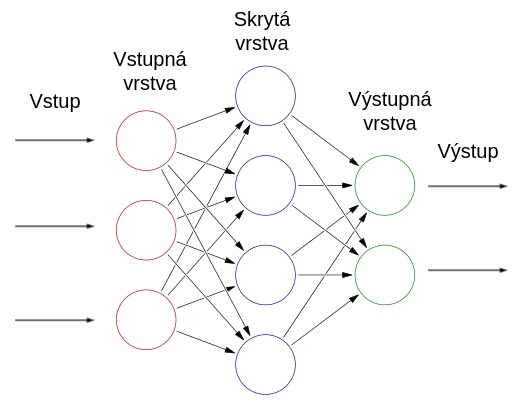
\includegraphics[scale=0.45]{simple_nn.jpg}\end{center}
		\caption[Jednoduchá neurónová sieť]{Príklad jednoduchej neurónovej siete}\label{simple_nn}
	\end{figure}

\subsubsection{Rekurentné neurónové siete}
Zložitejším typom  neurónových sietí sú rekurentné neurónové siete. Už z názvu vyplýva, že jednou z vecí, ktoré umožňujú, je rekurenciu. Vďaka nej prepojenia neurónov už nie sú jednosmerné len z jednej vrstvy na druhú, ale umožňuje prepojiť neuróny akokoľvek a tak vytvárať napríklad slučky či cykly (ukážka na obrázku \ref{rnn_image}).

\begin{figure}[H]
	\begin{center}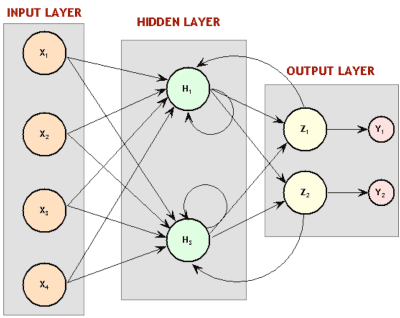
\includegraphics[scale=0.7]{rnn_model.png}\end{center}
	\caption[Jednoduchá rekurentná neurónová sieť]{Príklad jednoduchej rekurentnej neurónovej siete\label{rnn_image}\footnotemark}
	
\end{figure}
\footnotetext{http://www.mattmoocar.me/blog/RNNCountryLyrics/}

Vyššie uvedená funcionalita dovoľuje zachytiť aj dynamické časovo obmedzené správanie a používať kontext z minulosti, teda použiť niečo ako „pamäť“. Rekurentné siete majú veľké množstvo typov, od jednoduchších LSTM až po zložitejšie obojsmerné (z angl. bi-directional).

\paragraph{LSTM} 
LSTM\cite{gers1999learning} - skratka pre anglické pomenovanie Long short-term memory, čo v preklade znamená dlhá krátkodobá pamäť. Tento typ rekurentných sietí sa ukázal extrémne efektívny pri úlohách, kde je nutné pamätať si určitú informáciu (kratšieho charakteru) dlhý čas. Za to môžeme vďačiť LSTM jednotke, ktorej štandardná architektúra je zobrazená na obrázku \ref{lstm_unit_image}.

\begin{figure}[H]
	\begin{center}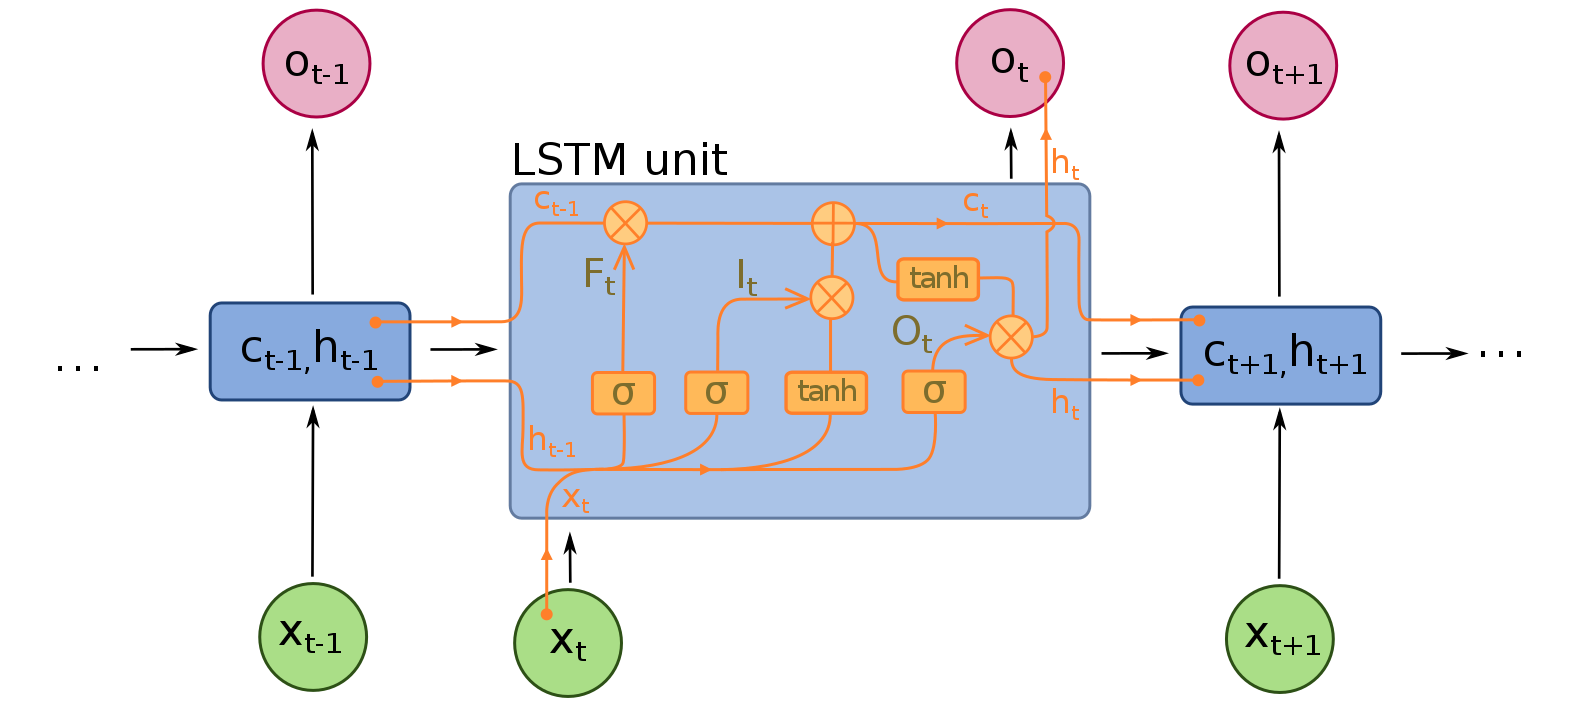
\includegraphics[scale=0.25]{lstm_unit.png}\end{center}
	\caption[Zobrazenie LSTM jednotky]{Ukážka štruktúry LSTM jednotky\label{lstm_unit_image}\footnotemark}
	
\end{figure}
\footnotetext{http://colah.github.io/posts/2015-08-Understanding-LSTMs/}

Na rozdiel od klasickejších rekurentných sietí, kde jednotka obsahuje jednu vrstvu neurónov, LSTM jednotka (bunka) obsahuje až štyri, každá špecializovaná na niečo iné. Na obrázku vyššie reprezentuje prvá horizontálna čiara v jednotke jej stav. Informácia tadiaľto prakticky len "tečie", s malými lineárnymi zmenami ako pridanie alebo odobratie. Tieto akcie sú opatrne regulované tzv. bránami.

Spodná horizontálna čiara reprezentuje postupné vstupy do štyroch vrstviev zobrazených na obrázku ako štvorce s aktivačnými funkciami ($\sigma$ - sigmoid, tanh). Vrstvy so sigmoid-om fungujú ako tzv. "strážcovia", vzhľadom na ich výstup v intervale \ <0,1> \ určujú aké veľké množstvo informácie má byť pustené ďalej (0 - nič, 1 - všetko). Týmto prakticky kontrolujú a udržujú stav celej bunky. Prvá sigmoid vrstva sa nazýva "zabúdacia brána" (z angl. forget gate layer) a určuje, aké množstvo informácií z aktuálneho stavu bunky bude zahodených. Druhá sigmoid vrstva sa nazýva "vstupná brána" (z angl. input gate layer) a určuje, ktoré hodnoty budú aktualizované. Tretia tanh vrstva vytvorí vektor hodnôt, ktoré je možné pridať k stavu bunky. Výstup z týchto dvoch vrstiev je skombinovaný k aktualizovaniu stavu bunky. Posledná sigmoid vrstva prakticky určuje aké hodnoty budú výstupom z celej jednotky. Výstup je založený na upravenom stave bunky, avšak vyfiltrovaný na základe hodnôt z poslednej sigmoid vrstvy.

Keďže rekurentné siete na rozdiel od dopredných môžu na vstupe spracovať aj ľubovoľnú sekvenciu (vektor) predstavujú s možnosťou "pamäte" \ značný posun. V praxi sa používajú napríklad pri úlohách so spracúvaním jazyka. Keby sme chceli napríklad predikovať nasledujúce slovo vo vete, je veľmi užitočné vedieť aké slová boli pred ním aby predikcia dávala zmysel. Práve v tejto oblasti sa LSTM siete ukázali veľmi efektívne. Využívajú sa ďalej napríklad aj pri rozpoznávaní reči\cite{rnn_speech} alebo písma\cite{rnn_handwriting}, či generovaní popisu k obrázkom\cite{image_description}, kedy však fungujú v kombinácii s konvolučnou neurónovou sieťou (z angl. convolutional neural network). Tá je ďalším typom sietí a v tomto prípade bola použitá na klasifikáciu obrázkov a rozpoznávanie objektov, LSTM sieť bola použitá iba na generovanie výsledného jednoduchého popisu.


\subsubsection{Konvolučné neurónové siete}
\
\
\
\
\
Základ tohto typu siete tvorí vstupná konvolučná vrstva\footnote{http://www.wildml.com/2015/11/understanding-convolutional-neural-networks-for-nlp/} s konvolučným filtrom, ten býva väčšinou malý (3x3, 5x5). Vstup tejto vrstvy musí byť v tvare \textit{m} x \textit{m} x \textit{r}, kde \textit{m} je šírka a výška obrázku, \textit{r} je počet farebných kanálov. Napríklad pre RGB obrázok je r=3 (červená, zelená, modrá). Konvolučným filtrom sa prejde celý obrázok a výstupom z tejto vrstvy je niekoľko filtrov. Tie sa potom spracúvajú v ďalšie vrstve združovania (z angl. pooling layer\cite{cs231n}), ktorá tieto filtre rozvzorkuje. To prebieha nezávisle na každom získanom filtri z konvolučnej vrstvy. Rozvzorkovanie v podstate znamená, že sa zmení veľkosť filtrov použítim operácie MAX. Najbežnejšou formou spomínanej vrstvy je verzia s oknom (filtrom) o veľkosti 2x2 aplikovaným s krokom veľkosti 2. Toto sa dá jednoducho vysvetliť ako prejdenie každého výstupu z konvolučnej vrstvy oknom uvedenej veľkosti postupne po 2 políčkach na šírku aj výšku, pričom z každej štvorice v okne sa získa MAX operáciou maximum, s ktorým sa pracuje ďalej. Na  obrázku\footnote{http://cs231n.github.io/convolutional-networks/} \ref{fig:cnn} je vidieť výsledok popisovaného postupu na jednoduchom príklade.
	
	\begin{figure}[H]
		\begin{center}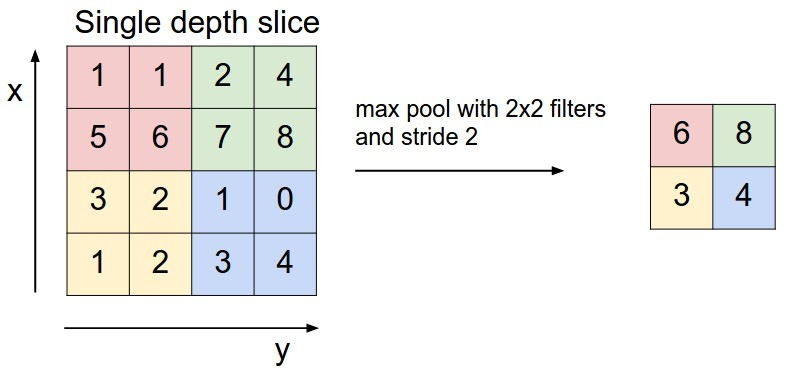
\includegraphics[scale=0.38]{maxpool.jpeg}\end{center}
		\caption[Vrstva združovania - príklad vzorkovania]{Príklad vrstvy združovania, pri ktorom sa rozvzorkuje výstup z konvolučnej vrstvy o veľkosti 4x4, filtrom 2x2, s krokom veľkosti 2 za použitia operácie MAX}\label{fig:cnn}
	\end{figure}
	Takýchto konvolučných vrstiev s vrstvami združovania môže byť aj viac, nemusia ani nutne nasledovať po sebe. Po týchto vrstvách nasleduje plne prepojená vrstva alebo vrstvy (z angl. fully-connected layers), čo je vrstva, v ktorej majú neuróny plné spojenie so všetkými aktiváciami v predošlej vrstve, rovnako ako pri bežných neurónových sieťach. Aktivačnou funkciou neurónov na tejto vrstve býva väčšinou ReLU. Po plne prepojenej vrstve (vrstvách) už nasleduje iba výstupná vrstva. Na obrázku\footnote{https://ujjwalkarn.me/2016/08/11/intuitive-explanation-convnets/} nižšie je jednoduchý náčrt vyššie popísané konvolučnej neurónovej siete. 
	\begin{figure}[H]
		\begin{center}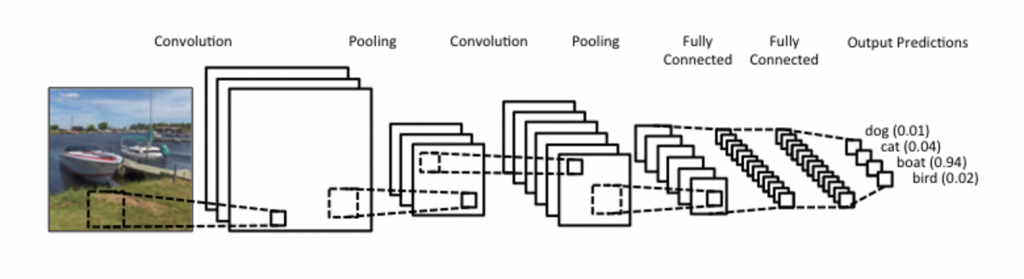
\includegraphics[scale=0.38]{cnn.png}\end{center}
		\caption[Konvolučná neurónová sieť]{Príklad konvolučnej neurónovej siete}\label{conv_nn}
	\end{figure}
	
	Využite tohto typu je v podstate všade, kde sa pracuje s obrázkami. Či už ide o automatické vyznačenie tvárí pre označenie na facebook-u, autonómne vozidlá, ktoré sa vedia riadiť sami (autopilot) alebo triedenie uhoriek na farmách v Japonsku\footnote{https://cloud.google.com/blog/big-data/2016/08/how-a-japanese-cucumber-farmer-is-using-deep-learning-and-tensorflow}. Na tento konkrétny softvér bol použitý príklad kódu jednoduchej konvolučnej siete z tutoriálu\footnote{https://www.tensorflow.org/versions/0.6.0/tutorials/mnist/pros/index.html} pre TensorFlow (knižnica pre prácu s neurónovými sieťami, popísaná v kapitole \ref{tf}), s modifikáciou konvolučnej a združovacej vrstvy tak, aby bola sieť uspôsobená počtu tried uhoriek (10) a ich formátu obrázkov. 
	
	Z mnohých pokusov o autonómnu jazdu stoja za zmienku hlavne tie od Tesly a Google. Prototyp autonómneho systému vozidla od Google-u Dave-2\cite{google_car} využíva model neurónovej siete s 9 vrstvami, jednu normalizačnú, 5 konvolučných a 3 plne prepojené vrstvy. Kamerami spracovaný obraz okolia s frekvenciou 10 snímkov za sekundu (tak nízky počet preto, aby sa predišlo veľkému množstvu príliš podobných obrázkov) je po jednom snímku rozdelený do YUV\footnote{farebný priestor používaný vo video aplikáciách} úrovní a posunutý do neurónovej siete.   
 
\subsubsection{Autoenkóder}
\label{autoencoder}
Autoenkóder (z angl. autoencoder) je špeciálnym typom neurónovej siete, tradične je používaný ako algoritmus učenia bez učiteľa. K učenia však požíva štandardný algoritmus spätného šírenia chyby, kedy sú ale cieľové hodnoty rovné tým vstupným, snaží sa teda naučiť funkciu:
\begin{equation}
	y^{(i)} = x^{(i)}
\end{equation}

Jeho cieľom je v podstate naučiť sa enkódovanú reprezentáciu dát, čo sa využíva napríklad pri komprimácii alebo k zníženiu dimenzionality dát\cite{autoencoder_dimensionality}. Autoenkóder sa skladá z dvoch častí (ako je to vidieť na obrázku \ref{autoencoder_graph}):
\begin{itemize}
	\item enkóder - prvá časť, postupne sa od vstupnej vrstvy zmenšuje počet neurónov, čo v podstate komprimuje vstupnú informáciu do enkódovanie reprezentácie
	\item dekóder - druhá časť, jeho vstupom je práve enkódovaná reprezentácia dát a jeho cieľom je z tejto reprezntácie zrekonštruovať pôvodné dáta
\end{itemize}
 
\begin{figure}[H]
	\begin{center}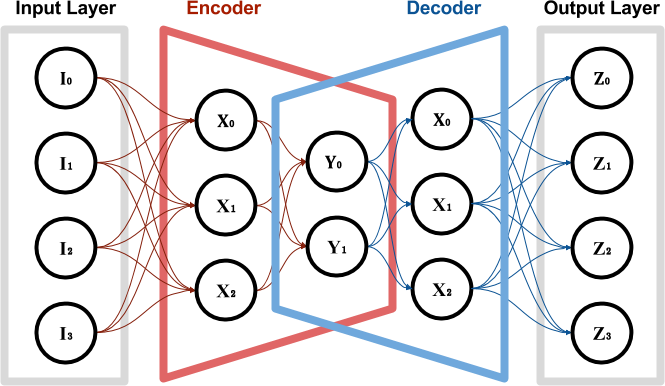
\includegraphics[scale=0.4]{autoencoder.png}
		\caption[Príklad jednoduchého autoenkóderu]{
			Diagram reprezentujúci jednoduchý autoenkóder\footnotemark
		}\label{autoencoder_graph}
	\end{center}
\end{figure}

\footnotetext{https://www.alanzucconi.com/2018/03/14/an-introduction-to-autoencoders/}

I keď cieľom je na konci mať na výstupnej vrstve dokonale zrekonštruovaný vstup, bohužiaľ to tak takmer nikdy nie je a pri autoenkóderoch sa tak jedná o stratovú kompresiu. Zatiaľ nie sú široko rozšírené a v praxi sa používajú najmä pri odstraňovaní šumu\cite{autoencoder_denoising} z dát alebo pri znižovaní ich dimenzionality. Uplatnenie tak nachádzajú hlavne pri spracovaní jazyka\cite{autoencoder_nlp} a počítačovom videní - napríklad pri detekcii objektov\cite{autoencoder_artur}.
 
\subsection{Framework-y pre prácu s neurónovými sieťami}
V dnešnej dobe moderného internetu a dostupnosti technológií máme možnosť výberu z dostatočného množstva framework-ov pre potreby riešenia najrôznejších problémov neurónovými sieťami. Pri výbere môžeme brať do úvahy napríklad preferencie operačného systému (Windows, Linux, ...), programovacieho jazyka (Python, C++, Java, ...), ale aj benefity distribuovaného riešenia a omnoho viac. V nasledujúcich podkapitolách sú preto popísané niektoré z najpoužívanejších technológií pre implementovanie neurónových sietí. 

\subsubsection{TensorFlow}
\label{tf}
TensorFlow\footnote{https://www.tensorflow.org/} je open-source softvérová knižnica, ktorá pre numerické výpočty používa graf dátového toku, kde uzly grafu reprezentujú matematické operácie a hrany multidimenzionálne dátové polia, tzv. tenzory. Graf je možné skonštruovať použitím jazykov s podporou frontend-u (C++, Python, ...). 

Flexibilná architektúra umožňuje vykonávať výpočty na CPU alebo GPU (nepomerne rýchlejšie) na serveroch, desktopových počítačoch či dokonca aj mobilných zariadeniach. Pôvodne bol TensorFlow vyvinutý výzkumníkmi a inžiniermi v Google-i pre strojové učenie a hlboké učenie, avšak jeho využitie je oveľa širšie. V súčasnosti používa TensorFlow veľké množstvo programov, napríklad Google vyhľadávač, prekladač alebo YouTube. 

Momentálne podporuje jazyky C++, Python, Java, Go, Swift.

Medzi hlavné výhody patrí:
\begin{itemize}
	\item podpora pre jednoducho naučiteľné jazyky (Python)
	\item použtie výpočtovej grafovej abstrakcie
	\item vizualizácie pomocou TensorBoard-u\footnote{https://www.tensorflow.org/programmers\_guide/summaries\_and\_tensorboard} (interaktívne grafy pre priebeh učenia, pre model siete, ...)
	\item dostatočne nízko-úrovňový pre plnú kontrolu a implementáciu vlastnej (novej nie len preddefinovanej) funkcionality (v porovnaní napríklad s framework-om Keras (kapitola \ref{keras}))
\end{itemize}

Ako nevýhody možno uviesť:
\begin{itemize}
	\item nedostatok predtrénovaných modelov
	\item pri použití s určitými jazykmi (Python, Java, ...) je pomalý, nakoľko sa nejedná najrýchlejšie jazyky
\end{itemize}

\subsubsection{Microsoft CNTK}
Označuje knižnicu Microsoft Cognitive Toolkit\footnote{https://docs.microsoft.com/en-us/cognitive-toolkit/}, ktorá zlepšuje modularizáciu a údržbu separácie výpočtových sietí, zároveň postkytuje algoritmy učenia a popisy modelov. Má sa jednať o odpoveď na TensorFlow, poskytovaná funkcionalita je veľmi podobná, avšak je o niečo rýchlejší. Princíp a celá architektúra sú zachytené na diagrame na obrázku \ref{cntk_image}. 

\begin{figure}[H]
	\begin{center}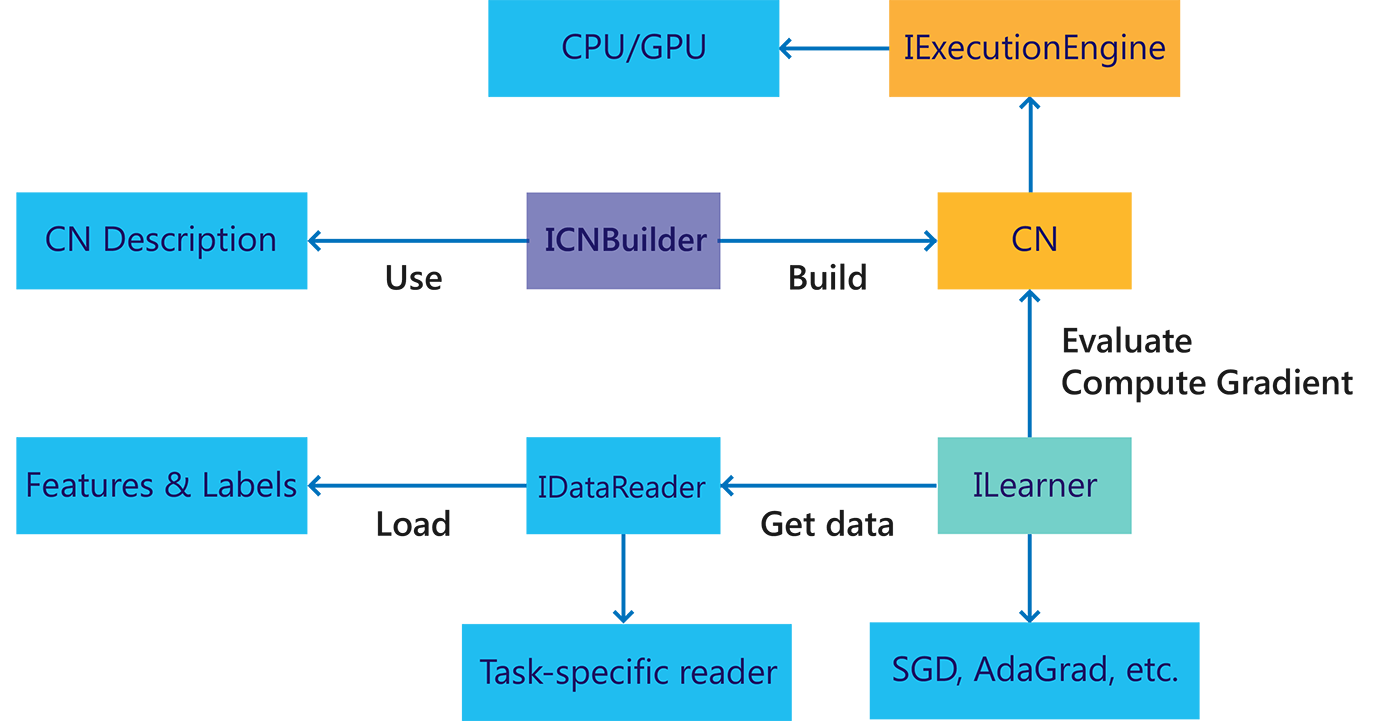
\includegraphics[scale=0.3]{microsoft-cntk-architecture.png}
		\caption[Architektúra fungovania Microsoft CNTK]{
			Diagram zobrazujúci architektúru fungovania Microsoft CNTK\footnotemark
		}\label{cntk_image}
	\end{center}
\end{figure}
\footnotetext{https://dzone.com/articles/progressive-tools10-best-frameworks-and-libraries}

Momentálne podporuje jazyky C++, C\#, Python, Java.

Výhodami tohto framework-u sú:
\begin{itemize}
	\item flexibilita
	\item umožňuje distribuovaný tréning
\end{itemize}

Medzi nevýhody možno zaradiť:
\begin{itemize}
	\item implementácia v novom jazyku, Network Description Language (NDL)
	\item nedostatok možností a nástrojov pre vizualizácie
\end{itemize}

\subsubsection{Theano}

Theano\footnote{https://github.com/Theano/Theano} je veľmi silná knižnica umožňujúca definovanie, optimalizáciu a evaluáciu numerických operácií nad multidimenzionálnymi poliami s obrovskou efektivitou. Podobne ako TensorFlow, k abstrakcii výpočtov používa grafy, ako možno vidieť na príklade na obrázku \ref{theano_image}.

% theano-data-visualization.png

\begin{figure}[H]
	\begin{center}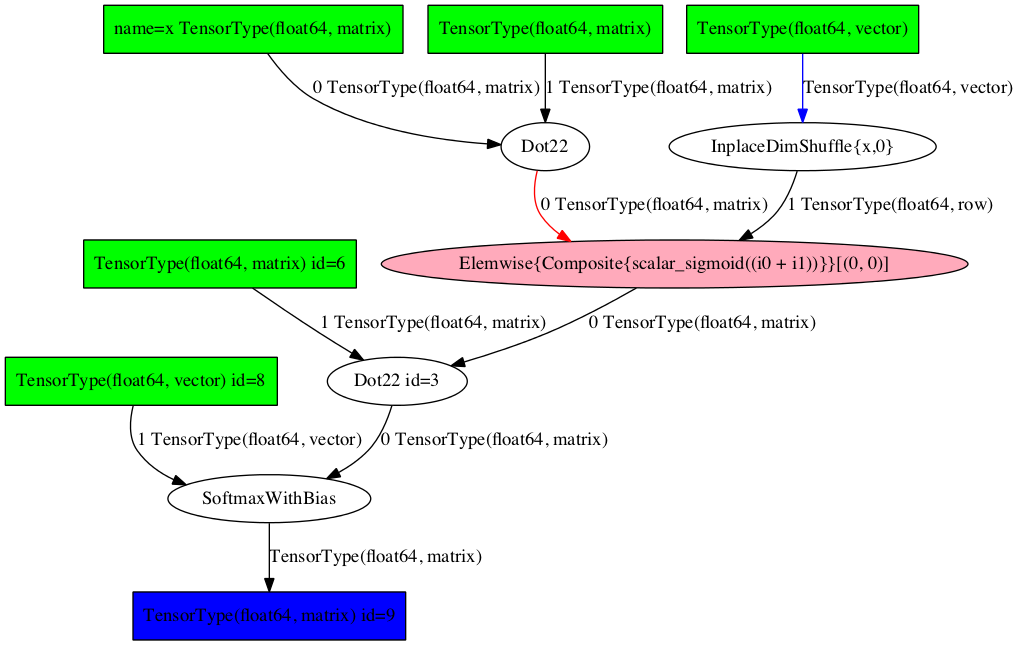
\includegraphics[scale=0.35]{theano-data-visualization.png}
		\caption[Príklad grafovej abstrakcie výpočtov použitím framework-u Theano]{
			Príklad grafovej abstrakcie výpočtov použitím framework-u Theano\footnotemark
		}\label{theano_image}
	\end{center}
\end{figure}
\footnotetext{http://www.wildml.com/2015/09/speeding-up-your-neural-network-with-theano-and-the-gpu/}

Momentálne podporuje iba programovací jazyk Python a v poslednej dobe vývoj tohto framework-u dosť upadá.

Medzi hlavné výhody patrí:
\begin{itemize}
	\item veľmi dobrá optimalizácia pre CPU a GPU (najmä vďaka použitiu nízko-úrovňovej funkcionality naprogramovanej v jazyku C)
	\item vysoko efektívna knižnica pre numerické úlohy
\end{itemize}

Za najväčšie nevýhody sú pokladané:
\begin{itemize}
	\item Theano samo o sebe je v porovnaní s ostatnými knižnicami príliš nízko-úrovňové
	\item potreba použitia s inými knižnicami s vyšším stupňom abstrakcie (napríklad Keras) 
\end{itemize}

\subsubsection{Keras}\label{keras}

Ďalší open-source framework pre prácu s neurónovými sieťami, avšak na rozdiel od predošlých troch nie je vypracovaný ako koncové riešenie pre strojové učenie. Namiesto toho slúži ako rozhranie a poskytuje vyššiu úroveň abstrakcie pre jednoduchšie používanie ostatných framework-ov, z ktorých momentálne pre použitie ako backend podporuje TensorFlow a Theano. Myšlienka stojaca za celým projektom je: \textit{"Byť schopný pretaviť myšlienku na výsledok s čo najmenším zdržaním je kľúčom k dobrému výskum"\footnote{https://keras.io/}}, čo bude aj jedným z dôvodov prečo je práca s ním jednoduchšia.

Keras je v súčasnosti možné používať iba v programovacom jazyku Python.

Jeho hlavnými výhodami sú:
\begin{itemize}
	\item jednoduchosť naučenia, používateľsky veľmi prívetivé
	\item ľahká rozšíriteľnosť
	\item bezproblémový beh aj na CPU aj na GPU
	\item bezproblémové fungovanie aj s Theano-m a aj s TensorFlow-om
	\item rýchle prototypovanie
\end{itemize}

Za jedinú nevýhodu može byť považovaná nemožnosť použitia ako nezávislý framework - vždy je potrebný nejaký ďalší backend.

\subsubsection{Spark MLlib}

Škálovateľná knižnica pre strojové učenie, široko využívaná najmä v distribuovaných systémoch hlavne kvôli svojej efektivite. Veľmi jednoducho je ju možné pripojiť do Hadoop workflow-u, poskytuje množstvo algoritmov pre strojové učenie optimalizovaných pre výpočty v už spomínaných distribuovaných systémoch na dátach vo veľkom meradle\footnote{https://spark.apache.org/mllib/}.

Momentálne poskytuje podporu pre jazyky Python, Java, Scala a R.

Najväčšími výhodami sú:
\begin{itemize}
	\item vysoká rýchlosť na dátach vo veľkom meradle
	\item dostupnosť v jazykoch, ktoré podobnými framework-ami nie sú často podporované
\end{itemize}

Za nevýhody možno pokladať:
\begin{itemize}
	\item strmá krivka učenia
	\item jednoduché používanie formou "pripoj a hraj" \ (z angl. plug-and-play) dostupné iba pre Hadoop
\end{itemize}

Nevýhodou v porovnaní s vyššie uvedenými framework-ami môže byť nižšie množstvo implementovaných algoritmov, avšak vývoj rozhodne nezaháľa a pridávanej funcionality je stále viac a viac.


\newpage

\section{Existujúce modely vizuálnej pozornosti}
\label{saliency_models}
Existujúce modely vizuálnej pozornosti možno z pohľadu typu predikovaných máp výraznosti rozdeliť na modely k predikcii pozornosti zdola nahor \ (kapitola \ref{bottom-up_modely}) a modely k predikcii pozornosti zhora nadol (kapitola \ref{top-down_modely}). Ako prínosná sa ale javí aj detekcia objektov (kapitola \ref{object_detection}) a modely postavené práve na nej. Ďalším zaujímavým rozdelením však je rozdelenie podľa použitých princípov a technológií \cite{polatsek}, na modely:

\begin{itemize}
	\item hierarchické - využívajú hierarchické rozkladanie príznakov
	\item Bayesove - využívajú kombináciu výraznosti s predchádzajúcimi znalosťami
	\item rozhodovaco-teoretické - využívajú diskriminačnú teóriu výraznosti
	\item informaticko-teoretické - využívajú maximalizáciu informácie z daného prostredia
	\item grafické - predikcia výraznosti je založená na grafových algoritmoch
	\item vzorovo klasifikačné - využívajú strojové učenie zo vzorov s výraznými črtami
\end{itemize}

\subsection{Modely k predikcii pozornosti zdola nahor}
\label{bottom-up_modely}
Nakoľko práve pozornosť zdola nahor bola prvá skúmaná, existuje k jej predikcii obrovské množstvo najrozličnejších modelov. Niekoľko z nich je popísaných v nasledujúcich podkapitolách. Porovnaním týchto rôznych typov by sa dalo povedať, že ako najlepšie a najpresnejšie sa javia nové moderné postupy strojového učenia. Ich nevýhodou však je potreba dostatočne veľkého datasetu, na ktorom by mohli byť natrénované ako aj značne dlhé trénovanie a predikcie v porovnaní s tými, ktoré používajú rôzne matematické postupy alebo extrakcie čŕt a príznakov, kde fáza trénovania nie je nutná.

\subsubsection{Itti-ho model}

Itti-ho model\cite{itti} je jedným z najznámejších modelov vizuálnej pozornosti, i keď patrí medzi tie staršie, dodnes je široko používaný a citovaný v mnohých článkoch. Je to biologicky inšpirovaný bottom-up model, ktorý využíva hierarchické rozloženie vlastnosí a ich kombináciu do výslednej mapy výraznosti (z angl. saliency map). Ako je vidieť na obrázku \ref{itti_image}, zo vstupného obrázka sa vytvoria 3 typy máp a to podľa farby, intenzity a orientácie, ktorých kombináciou sa dosiahne už spomenutá mapa výraznosti. 

\begin{figure}[H]
	\begin{center}
		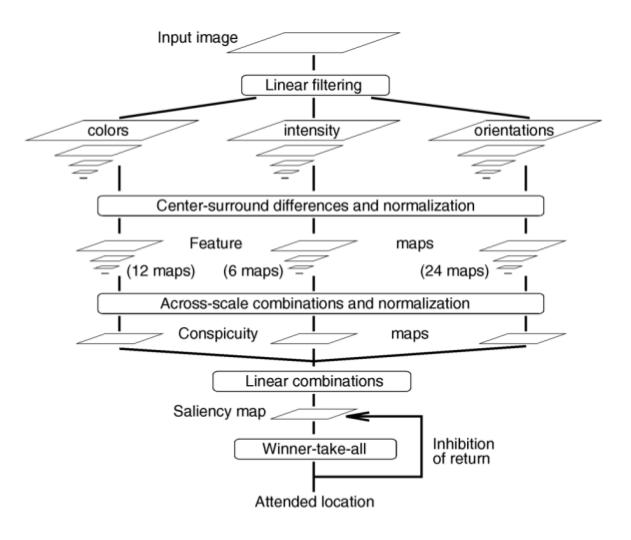
\includegraphics[scale=0.4]{itti_model.jpeg}
	\end{center}
	\caption[Itti-ho hierarchický model vizuálnej pozornosti]{Itti-ho hierarchický model vizuálnej pozornosti\cite{itti}\label{itti_image}}
\end{figure}

\subsubsection{Metóda hierarchickej výraznosti}

Pri použítí metódy hierarchickej výraznosti (z angl. hierarchical-saliency method\cite{gao2013hierarchical}) sa v podstate jedná o detekciu charakteristík v prirodzenej scéne. Tento postup je istým vylepšením predchádzajúceho Ittiho modelu a prakticky pozostáva z nasledujúcich dvoch krokov:

\begin{itemize}
	\item \textit{prvý krok} - extrakcia globálne výrazných oblastí (z angl. globally salient
	regions):
		\begin{enumerate}
			\item výpočet mapy výraznosti \textit{S} zo vstupného obrázka \textit{I}
			\item evaluácia oblastí záujmu (z angl. regions of interest, ROIs), automatická
			klasifikácia všetkých pixelov do dvoch kategórií k získaniu masky \textit{M}:
			\begin{itemize}
				\item[-] globálne výrazné oblasti (\textit{1})
				\item[-] zvyšok (\textit{0})
			\end{itemize}
			\item vynásobenie masky \textit{M} so vstupným obrázkom \textit{I} k získaniu filtrovaného
			obrázka \textit{I'}
		\end{enumerate}
	\item \textit{druhý krok} - evaluácia lokálne výrazných častí vo vnútri globálne výrazných
	oblastí. Použije sa vyfiltrovaný obrázok \textit{I'} z predchádzajúcich krokov k získaniu novej mapy výraznosti \textit{S'}, ktorá je finálnou mapou.
\end{itemize}
	
\subsubsection{Model pre určovanie salientných oblastí webových stránok}

Veľmi zaujímavým riešením pre predikciu a určovanie salientných oblastí scény v doméne webových stránok je model od Chengyao Shen a Qi Zhao\cite{Saliency} využívajúci metódy strojového učenia. Model je postavený na použití metódy MKL (Multiple Kernel Learning - kombinuje viacero jadier SVM (Support Vector Machine) miesto jedného), ktorá bola 
trénovaná na princípe binárneho regresného problému. Rozdiel oproti predošlým popisovaným modelom je však v tom, že predikovaná nebola priamo výsledná mapa výraznosti ale iba vektor pohľadov (fixácií) na vstupné obrázky, na základe ktorého bola potom spomínaná mapa vypočítaná. Autori po vyhodnotení výsledkov zistili že ako najviac salientné oblasti sa v scéne javia v prvom rade ľudská tvár, oči a celkovo vrchná časť ľudského tela. Zaujímavým vylepšením ich modelu však bolo to, že tieto zistenia zapracovali formou predtrénovania MKL na tieto vysoko salientné oblasti. 


\subsection{Modely k predikcii pozornosti zhora nadol}

\label{top-down_modely}
Predikcia pozornosti zhora nadol (top-down) je značne zložitejšia, nakoľko sa do úvahy berie aj sématický kontext scény. Tým môže byť napríklad emočný obsah (kapitola \ref{emotion_content}), či hľadanie konkrétnych objektov v scéne (kapitola \ref{caption_model}).


\subsubsection{Zameranie na emočný obsah}
\label{emotion_content}
Niekoľko riešení sa v posledných rokoch pokúsilo o predikovanie pozornosti zhora nadol (top-down) na základe emočného obsahu v pozorovanej scéne. Z nich stojí za zmienku napríklad model od Liu a spol. \cite{liu2016improving}, ktorí sa zamerali na spomínaný emočný obsah v rôznych oblastiach (blokoch) obrázka, kde do úvahy brali:
\begin{itemize}
	\item emočné objekty, napr. hady a krv (evokujú silný strach)
	\item výrazy tváre
	\item všeobecný emočný obsah
\end{itemize}

Hlavné problémy, ktoré riešili, by sa dali zhrnúť do dvoch otázok:
\begin{itemize}
	\item Ako získať a ohodnotiť intenzitu emócií pre obrázok?
	\item Aký typ emócie by mal byť dominantným pre jednotlivé obrázky?
\end{itemize}

Ich narhované riešenie malo niekoľko častí. Prvou je extrakcia faktorov pozornosti zdola nahor (bottom-up) vo forme nízko-úrovňových máp výraznosti založených na črtách a mapy priestorovej polohy s dôrazom na centrum pre výpočet odhadu hustoty pohľadu (z angl. gaze density estimation). K tomuto boli použité klasické hierarchické modely pre určovanie pozornosti (napr. Itti-ho model).

Druhou časťou je detekcia emócií, k čomu bol použitý emočný detektor založený na učení s použitím učenia viacerých inštancií (z angl. multiple instance learning, MIL) zo slabo oštítkovaných dát. Tými boli obrázky označené emočným typom\footnote{jedna z 8 skupín, do ktorých boli rozdelené emócie. Príkladom týchto skúpín sú napr. hnev, láska, smútok, prekvapenie, atď.}, ktorý bol určený po vypočítaní pravdepodobnosti vyskýtu jednotlivých typov pre každú časť obrázka. Touto matematickou operáciou sa autorom podarilo úspešne vyriešiť problém určenia dominantného typu emócie pre obrázok.  Ďalej bol pre zlepšenie extrakcie emócií použitý mechanizmus založený na SVM, ktoré bolo použité na detekciu ľudských tvárí a odhadnutie intenzity výrazu. Výstupom z tejto časti je emočná mapa, ohodnocujúca intenzitu emócií, určená pre ďalšie spracovanie.

Treťou časťou bolo spracovanie výstupov z predošlých dvoch častí lineárnym SVM, ktoré vo výsledku z faktorov pozornosti zdola nahor (bottom-up) a emočných faktorov vygeneruje výslednú mapu hustoty pohľadu (z angl. gaze density map). Vyššie popísaný postup je zobrazený na diagrame na obrázku \ref{liu_image}.

\begin{figure}[H]
	\begin{center}
		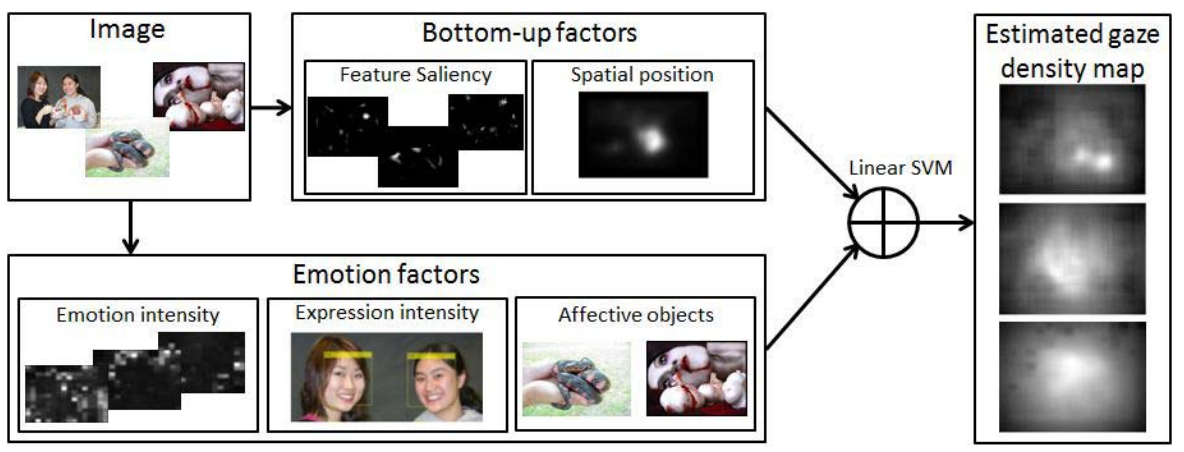
\includegraphics[scale=0.43]{liu_emotion_model.PNG}
		\caption[Diagram modelu k predikcii máp výraznosti založených na emočnom obsahu]{Diagram modelu od Liu a spol. k predikcii máp výraznosti založených na emočnom obsahu\cite{liu2016improving}\label{liu_image}}
	\end{center}
\end{figure}

Za veľkú výhodu tohto riešenia by sa dala pokladať kombinácia viacerých faktorov (aj pozornosti zdola nahor (bottom-up) aj pozornosti zhora nadol (top-down emočné faktory)  do výslednej mapy, vďaka čomu sa viac priblíži k reálnej pozornosti. Ako vieme tú neovplyvňujú čisto len jedny alebo druhé faktory, ale vždy je to ich kombinácia. Ako mierna nevýhoda by sa mohlo javiť rozdelenie emócií iba na 8 typov a určenie ako dominantný typ len jeden z nich, pričom ostatné sa ďalej neberú do úvahy.  


\subsubsection{SAM}
\label{sam}
SAM - skratka pre Saliency Attentive Model\cite{cornia2016predicting}, ďalší z modelov schopných aj predikcie pozornosti zhora nadol (top-down). Založený je na architektúre nazvanej ML-Net (Multi-Level Network\cite{cornia2016deep}), ktorá miesto klasických konvolučných vrstiev využíva dilatované konvolučné vrstvy, ktoré limitujú efekt zmenšovania. Táto architekúra použitá pre spracovanie vstupného obrázka je nasledovaná konvolučnými LSTM vrstvami, ich naučené výstupy potom spracováva už klasická konvolučná vrstva, výstupom ktorej je mapa výraznosti. Popisovaný postup je zobrazený na obrázku \ref{dilated_model_image}.

\begin{figure}[H]
	\begin{center}
		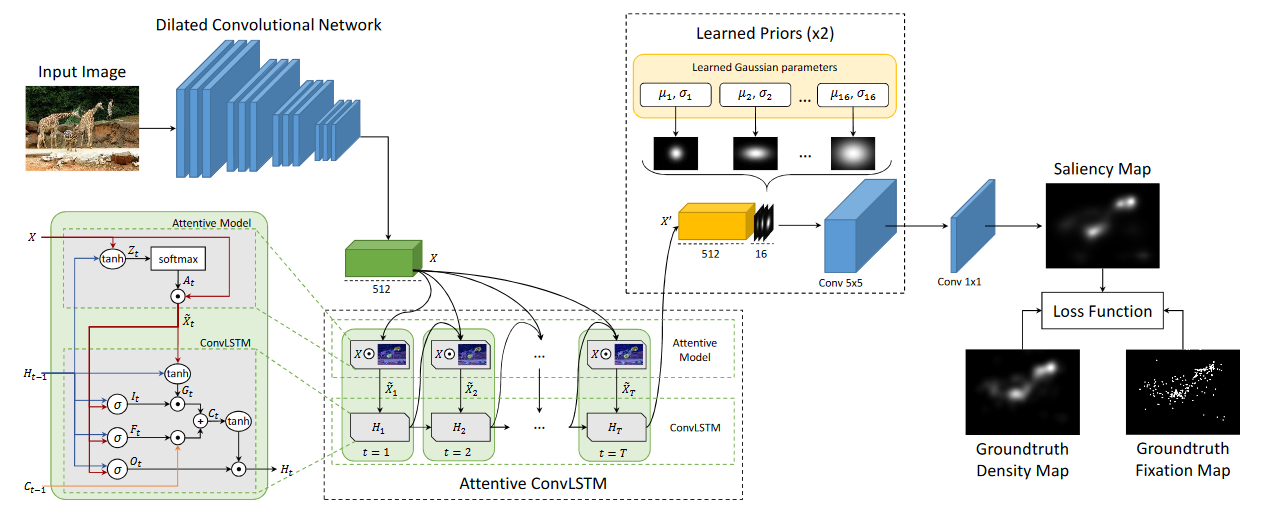
\includegraphics[scale=0.41]{dilated_NN.PNG}
		\caption[Diagram konvolučnej LSTM siete]{Diagram modelu využívajúceho dilatované konvolučné vrstvy v kombinácii s LSTM vrstvami \cite{cornia2016predicting}\label{dilated_model_image}}
	\end{center}
\end{figure}

Vďaka architektúre zobrazenej na obrázku vyššie je možné nezávisle na sebe trénovať dilatovanú konvolučnú sieť (alebo použiť predtrénovanú, či o niečo inú) a konvolučnú LSTM sieť. Veľkou výhodou dilatovanej konvolučnej siete je stratégia zväčšenia výstupného rozlíšenia obrázka, zatiaľ čo sa zachováva mierka, na ktorej operujú konvolučné filtre a počet parametrov. To je rozdiel oproti klasickej konvolučnej sieti, kedy je vstupný obrázok po extrakcii čŕt obvykle zmenšený, čo môže značne zhoršiť presnosť predikcie máp výraznosti.

Spomínané LSTM vrstvy (podrobnejšie zobrazené aj na obrázku \ref{dilated_model_image}) využívajú kombináciu aktivačných funkcií \textit{softmax}, \textit{tanh} a \textit{sigmoid}, kedy pri spracúvaní sekvenčne aktualizujú svoj interný stav. Ako vstup dostanú vektor extrahovaných čŕt z dilatovaných konvolučných vrstiev (\textit{X}), ktoré spracúvajú vstupné obrázky, a generovanú mapu výraznosti z predošlej LSTM vrstvy (s výnimkou prvej). Táto generovaná mapa je ešte upravená mechanizmami pozornosti, ktoré sa selektívne zameriavajú na rôzne časti obrázku. Vo výsledku je potom vektor extrahovaných čŕt (\textit{X}) a upravená generovaná mapa (\textit{$X_t$}) z predošlej vrstvy ešte ďalej spracovávaná aktivačnými funkciami \textit{tanh}.

Výstup z týchto vrstiev je ďalej upravený štandardnými konvolučnými vrstvami do výsledných máp výraznosti.

Ďalšou zaujímavou vecou na tomto riešení je zvolenie funkcie chyby (z angl. loss function). Autori nepoužili žiadny z tradičnejších typov, ale použili lineárnu kombináciu troch rôznych evaluačných metrík (popísané v kapitole \ref{metric}), v tvare:

\begin{equation}
	L (y, y^{den}, y^{fix}) = \alpha L1(y, y^{fix}) + \beta L2(y, y^{den}) + \gamma L3(y, y^{den})
\end{equation}

Pre vyššie uvedené platí:

$y$ - predikovaná mapa výraznosti

$y^{den}$ - pravdepodobnostná distribúcia (z angl. groundtruth density distribution)

$y^{fix}$ - binárna mapa fixácií

$\alpha, \beta, \gamma $ - tri skalárne hodnoty určené k vybalancovaniu troch funkcií chyby

$L1, L2, L3$ - tri funkcie pre výpočet evaluačných metrík, za radom Normalizovaná cesta výraznosti (NSS, z angl. Normalized Scanpath Saliency), Lineárny korelačný koeficient (CC), Kullback-Leiblerova divergencia (KL-Div), všetky bližšie popísané v kapitole \ref{metric}.

Za veľkú výhodu tohto riešenia pokladáme možnosť predikcie aj oboch typov pozornosti, v závislosti od datasetu, na ktorom je model natrénovaný. Taktiež možnosť nezávislej výmeny submodelov (dilatovaná konvolučná sieť,  konvolučná LSTM sieť) sa javí ako veľmi výhodná, keďže uľahčuje protypovanie bez nutnosti nového natrénovania celého modelu. Za miernu nevýhodu možno považovať značnú komplexitu modelu a s tým spojené nároky na hardvér, rovnako ako aj na čas nutný na natrénovanie od nuly, v prípade, že nechceme použiť predtrénované modely. 

\subsubsection{Pozornosť zhora nadol vedená titulkami}
\label{caption_model}
Jedným z ukážkových príkladov pozornosti zhora nadol (top-down) je úloha nájdenia nejakého konkrétneho objektu v scéne, čím sa inšpirovali výskumníci z Bostonskej univerzity. Predstavili model\footnote{http://ai.bu.edu/caption-guided-saliency/} \cite{ramanishka2017top} schopný predikcie máp výraznosti na základe kľúčových slov v zadanej vete a príslušnom obrázku alebo videu, príklad predikcií možno vidieť na obrázku \ref{top_down_captions_image}.

\begin{figure}[H]
	\begin{center}
		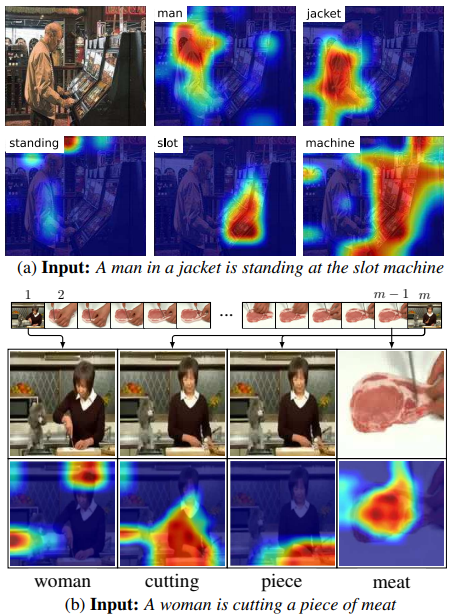
\includegraphics[scale=0.7]{top_down_captions.PNG}
		\caption[Predikcia salientných oblastí na základe kľúčových slov vo vete]{Predikcia salientných oblastí na základe kľúčových slov vo vete, hore po \textbf{a} predikcia pre obrázok, dolu po \textbf{b} predikcia pre video\cite{ramanishka2017top}\label{top_down_captions_image}}
	\end{center}
\end{figure}

Autori použili prístup nazvaný titulkami vedená vizuálna pozornosť (z angl. Caption-Guided Visual Saliency), ktorý produkuje mapy výraznosti pre nepohyblivé obrázky alebo video. Ako základný model použili LSTM enkóder-dekóder (z angl. encoder-decoder), ktorý predikuje aj dočasné (z videa) aj priestorové (z obrázkov) salientné mapy na základe kľúčových slov vo vete (vstupné titulky, popis) a mapuje ich na vstupné obrázky (alebo video). Vstupné titulky sú spracovávané LSTM vrstvami. Na obrázku \ref{top_down_captions_model_image} je možné vidieť načrtnutý model riešenia. Ako prvá vstupná vrstva funguje konvolučná neurónová sieť reprezentujúca enkóder pre video, ktorá "zakóduje" \ reprezentáciu obrázkov aj s aktiváciami všetkých vizuálnych konceptov detekovaných vo videu. Tieto informácie posunie ďalej ako vektor pre LSTM vrstvy reprezentujúce dekóder - ten rozhoduje o tom, ktoré časti použije pomocou LSTM výstupných brán k predikcii mapy výraznosti pre kľúčové slovo v čase \textit{t}. Autori ďalej zvolili veľmi šikovné riešenie pre predikciu máp len pre obrázky - jednoducho výstup produkovaný poslednou konvolučnou vrstvou zmenili na tzv. "dočasnú" sekvenciu (vektor): $V = (v_1, . . . , v_m)$. Tá je vytvorená sekvenčne scan-ovaním obrázka riadok po riadku z ľavého horného rohu do pravého dolného rohu. Prvá LSTM vrstva potom tento upravený vektor spracuje a posunie ďalej k dekódovaniu na kľúčové slová vo vete.

\begin{figure}[H]
	\begin{center}
		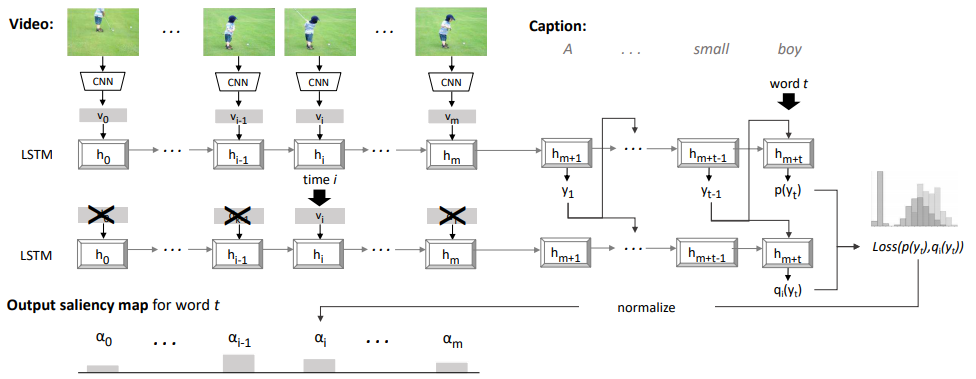
\includegraphics[scale=0.52]{top_down_captions_NN.PNG}
		\caption[Model neurónovej siete pre predikciu na základe kľúčových slov]{Diagram modelu neurónovej siete\cite{ramanishka2017top}, zhora vstup vľavo vo forme videa, vpravo titulky k nemu. V strede LSTM vrtvy neurónovej siete, dolu výstupná mapa výraznosti pre kľúčové slová. \label{top_down_captions_model_image}}
	\end{center}
\end{figure}

Popisované riešenie je ukážkovým modelom pre predikciu pozornosti počas hľadania objektov v scéne. Veľkou výhodou je použitie LSTM vrstiev pre zachytenie predošlého kontextu ako aj možnosť predikcie pre video aj obrázky iba s minimálnymi zmenami.

\subsubsection{Redukcia sémantických medzier pri predikcii vizuálnej pozornosti}

\label{semantic_gap}

Riešenie od Huang a spol. \cite{salicon_semantic_gap} sa zaoberalo zachytením sémantického kontextu scény ako prvku pozornosti zhora nadol, keďže práve to chýba v starších modeloch pre predikciu vizuálnej pozornosti. Pristúpili k tomu za použitia dvoch neurónových sietí (obrázok \ref{semantic_gap_nn}), ktorých predikcie na konci spojili pomocou spojovacej vrstvy do výslednej mapy vizuálnej pozornosti.  

\begin{figure}[H]
	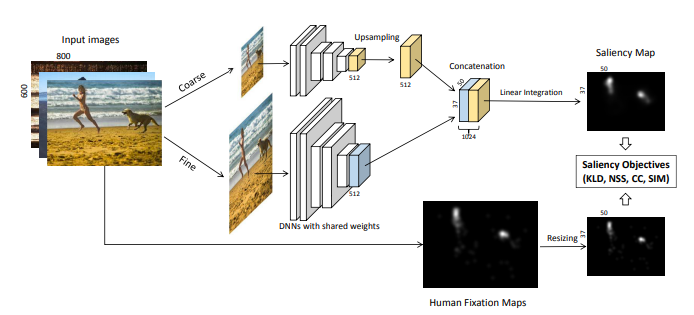
\includegraphics[scale=0.7]{semantic_gap_nn.PNG}
	\caption[Model redukcie sémantických medzier pri predikcii pozornosti]{Náčrt architektúri pri predikcii dvoch sietí so spojením výsledku do jednej mapy vizuálnej pozornosti}\label{semantic_gap_nn}
\end{figure}

Riešenie sa prakticky skladá z 2 častí a to z:
\begin{itemize}
	\item tzv. "hrubozrnnej" (z angl. coarse) - je zameraná na detekciu centier výrazných veľkých regiónov pozornosti, vstupom je menší obrázok
	\item tzv. "jemnozrnnej" (z angl. fine) - je zameraná na detekciu salientných oblastí menšej veľkosti, vstupom je vačší obrázok
\end{itemize}

Autori experimentovali s architektúrami sietí pre detekciu objektov (s časti popisované v kapitole \ref{object_detection}) ako napríklad AlexNet \cite{alexnet}, VGG-16 \cite{vgg16} a GoogLeNet \cite{googlenet}). Najlepšie predikcie mala kombinácia VGG-16 siete, čím sme sa neskôr pri experimentovaní inšpirovali. 

\subsection{Detekcia objektov}
\label{object_detection}
Z pohľadu modelov vizuálnej pozornosti môžu za zmienku stáť aj modely pre detekciu objektov a ich klasifikáciu, ktorých je dostupné značné množstvo aj predtrénovaných. Ako príklad si môžeme uviesť konvolučnú sieť VGG16\cite{vgg_net} určenú práve pre klasifikáciu objektov na obrázku. Skladá sa z 16 konvolučných vrstiev a veľkého množstva filtrov, ako možno vidieť na obrázku \ref{vgg_net_model}. Spracováva obrázky o veľkosti \textit{224x224}, bola trénovaná na 4 GPU 2-3 týždne a skladá sa zhruba zo 138 miliónov parametrov\footnote{https://medium.com/@sidereal/cnns-architectures-lenet-alexnet-vgg-googlenet-resnet-and-more-666091488df5}.  Je častou voľbou pre ďalšie experimentovanie v oblasti pre svoju presnosť a dostupnosť už natrénovaného modelu.

\begin{figure}[H]
	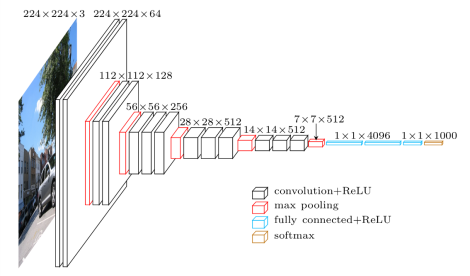
\includegraphics[scale=0.8]{vgg_net.png}
	\caption[VGG16]{Štruktúra neurónovej siete VGG-Net\footnotemark}\label{vgg_net_model}
\end{figure}

\footnotetext{https://www.quora.com/What-is-the-VGG-neural-network}

\subsubsection{Autoenkóder s VGG16 sieťou}

Ďalším zaujímavým riešením detekcie objektov v obrázku je autoenkóder od A. Meyer-a\cite{autoencoder_artur}, ktorý využíva aj vyššie popisovanú sieť VGG16. Využil princíp konvolúcie-dekonvolúcie kedy práve VGG16 funguje ako enkóder a jej v podstate zrkadlová podoba s dekonvolučnými vrstvami funguje ako dekóder (zobrazené na obrázku \ref{autoencoder_artur_graph})

\begin{figure}[H]
\centering	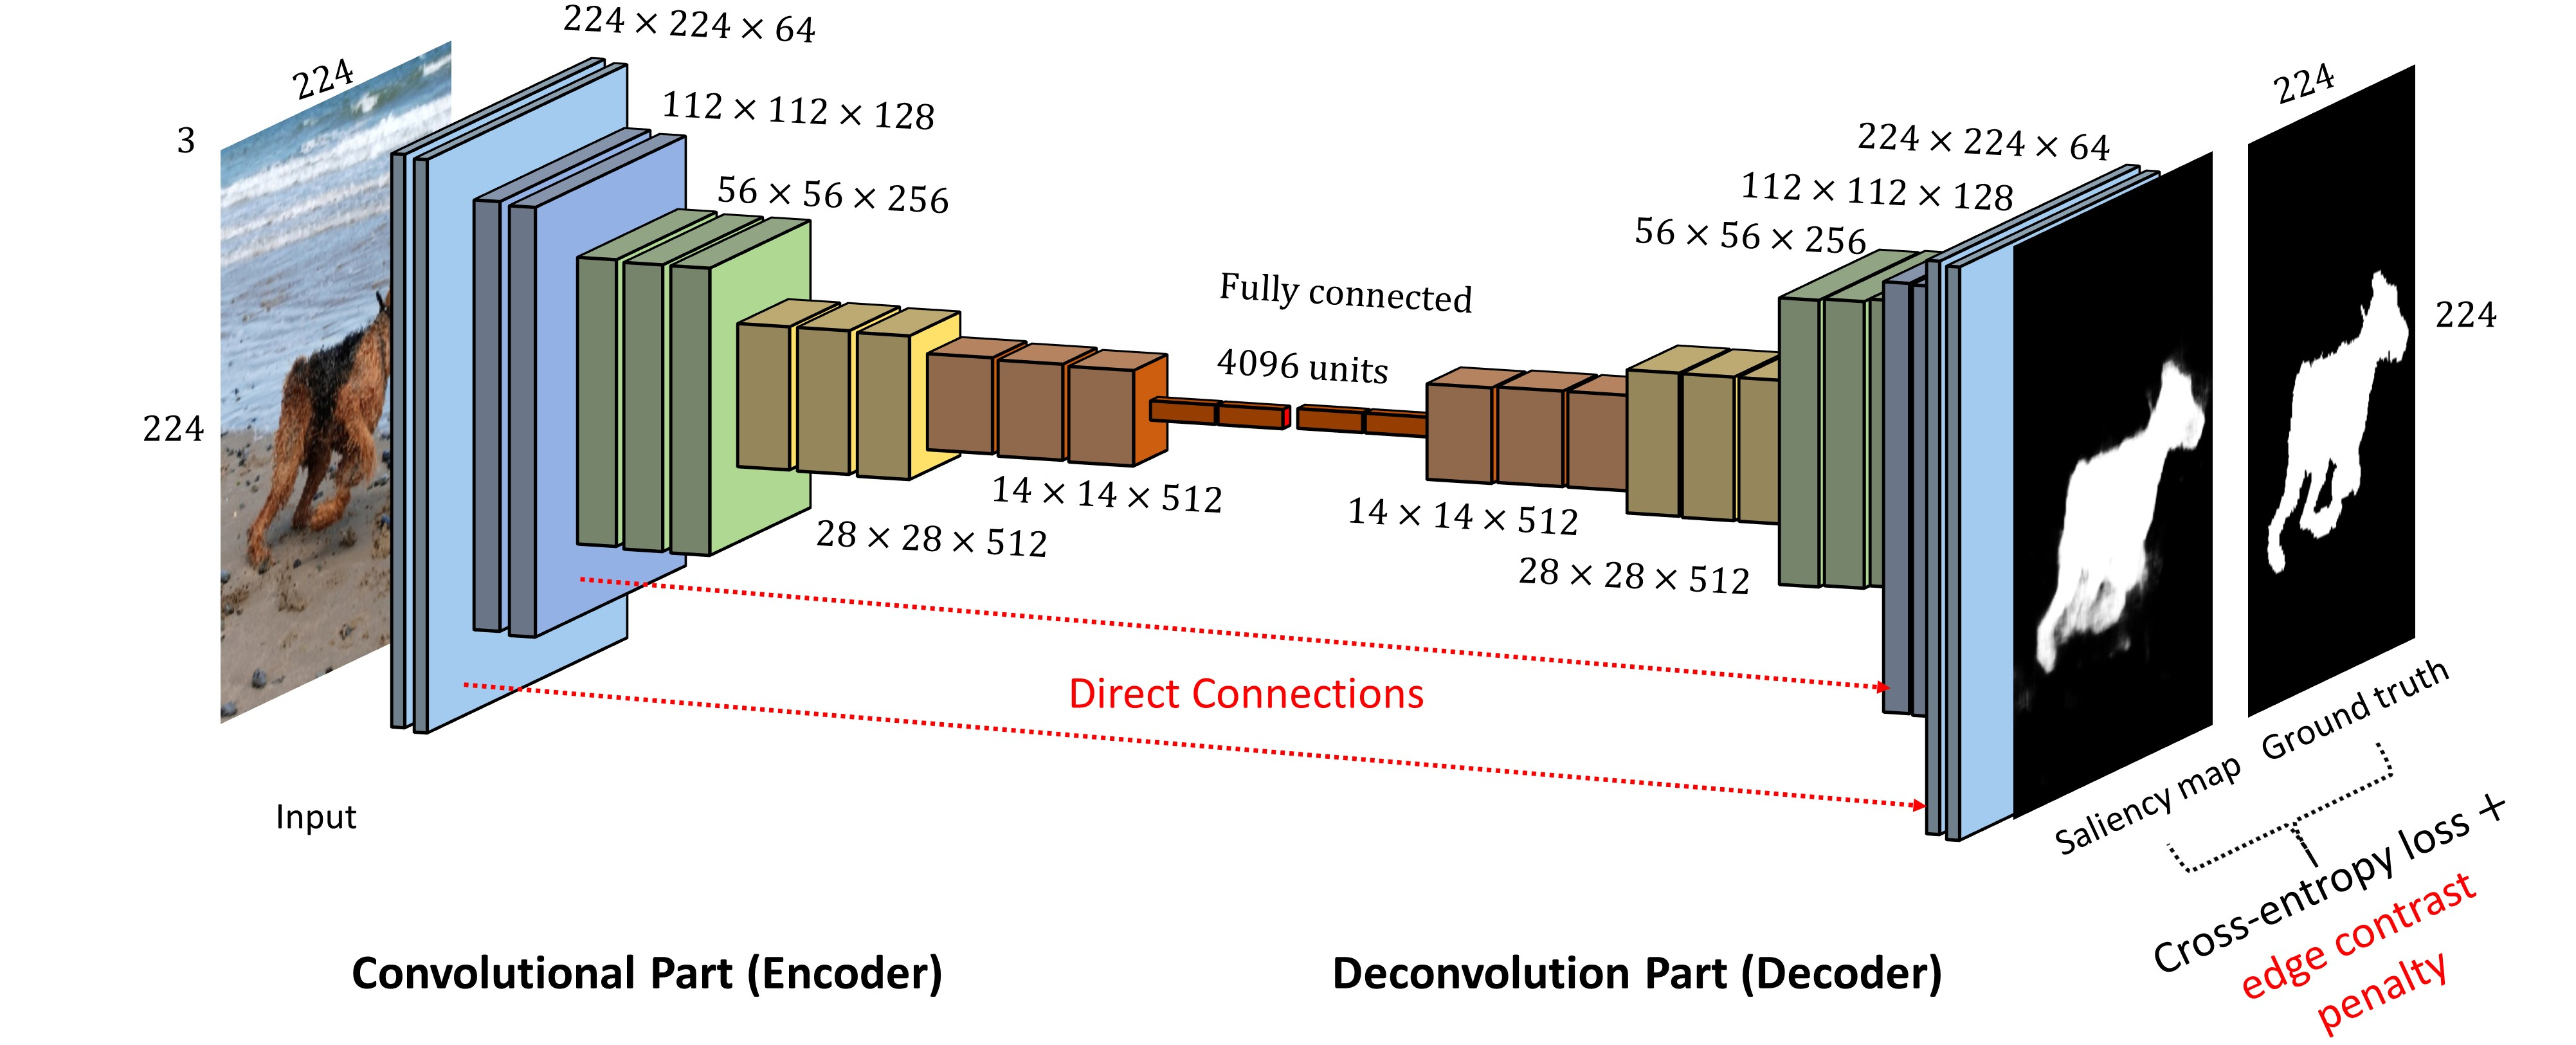
\includegraphics[scale=0.12]{autoencoder_artur.jpg}
	\caption[Autoenkóder pre detekciu objektov]{Štruktúra autoenkóderu pre detekciu objektov\footnotemark}\label{autoencoder_artur_graph}
\end{figure}

\footnotetext{https://github.com/arthurmeyer/Saliency\_Detection\_Convolutional\_Autoencoder}

Sieť je schopná aj priamych prepojení z konvolučných do dekonvolučných vrstiev a predikuje v podstate binárny obrázok, kde hodnota 1 reprezentuje pixel nájdeného objektu. Veľkou výhodou pri takejto sieti je možnosť použitia predtrénované modelu VGG16 pre enkóder. 

\subsubsection{Vedená a upravená vizuálna pozornosť}
\label{relu_and_guided_saliency}
Pri natrénovaných modeloch k detekcii objektov vieme pár jednoduchými zmenami docieliť, aby sme z nich dostali salientné mapy. Ako ukázali Springenberg a spol. \cite{springenberg2014striving}, stačí zmeniť aktivačné funkcie a upraviť algoritmus spätného šírenia chyby. K tomu môžeme použiť dva spôsoby, vďaka ktorým dostaneme dva typy vizuálnej pozornosti:

\begin{itemize}
	\item upravená alebo dekonvolučná (z angl.  rectified or deconv saliency \cite{zeiler2014visualizing}) - v algoritme spätného šírenia chyby sa odsekávajú negatívne gradienty a propaguje sa len pozitívny gradient pri zvýšení výstupných hodnôt
	\item vedená vizuálna pozornosť (z angl. guided saliency) - podobne ako pri predošlom type sa odsekávajú negatívne gradienty, propaguje sa však pozitívny gradient zodpovedný za pozitívne aktivácie
\end{itemize}

Po týchto zmenách vieme z vybraných konvolučných vrstiev dostať rôzne aktivácie a črty určitých filtrov, z ktorých potom po ďalších úpravách a spojeniach získame salientné mapy. Hoci celkovo tieto mapy nemusia byť veľmi presné, toto riešenie je vhodné ako začiatok pri kritickom nedostatku dát, keďže využíva už natrénované modely detekcie objektov. Tie sú voľne dostupné pre najrôznejšie experimentovanie. 


\newpage
\null
\thispagestyle{empty}
\newpage

\section{Datasety vizuálnej pozornosti}
\label{datasets}
Pre problém predikcie vizuálnej pozornosti existuje niekoľko voľne dostupných datasetov, ktoré sa líšia kvalitou, veľkosťou obrázkov, počtom fixácií či experimentami, pri ktorých boli zozbierané. Medzi najpoužívanejšie patria:

\begin{itemize}
	\item CAT2000\cite{cat2000}:
		\begin{itemize}
			\item obsahuje 4000 obrázkov z 20 rôznych kategórií
			\item obsahuje pohľady 24 ľudí počas 5 sekúnd
			\item obrázky sú naozaj rôznorodé, sú medzi nimi aj rôzne fraktály a obstraktné umenie
			\item veľkosť obrázkov je \textit{1920x1080}
		\end{itemize} 
	\item MIT1003\cite{mit1003}:
		\begin{itemize}
			\item 1003 obrázkov prírodných a vonkajších scén (779 krajina, 228 portrét)
			\item obsahuje pohľady 15 ľudí počas 3 sekúnd
			\item veľkosť obrázkov je rôznorodá, od menších až po HD obrázky
		\end{itemize} 
	\item SALICON\cite{salicon}
		\begin{itemize}
			\item vizuálna pozornosť v kontexte (z angl. Saliency in Context)
			\item obsahuje obrázky z datasetu MS COCO\footnote{http://cocodataset.org}, tie obsahujú neikonické pohľady a objekty v kontexte
			\item pozostáva z 10 000 trénovacích, 5 000 validačných a 5 000 testovacích obrázkov 
			\item veľkosť obrázkov je \textit{1920x1080}
		\end{itemize} 
	\item DUT-OMRON\cite{dut-omron}:
		\begin{itemize}
			\item obsahuje viac než 5000 obrázkov
			\item obsahuje pohľady 5 ľudí za prvé 2 sekundy
			\item má odstránené extrémy v dátach (z angl. outliers)
			\item viac ako 95\% obrázkov má viac než 50 fixácií
			\item všetky obrázky nemajú iba jeden veľký objekt v strede - t.j. fixácie nie sú stále koncentrované v tej istej oblasti
			\item veľkosť obrázkov je \textit{400x300}
			\item má dobre štruktúrovane spracované dáta
		\end{itemize} 
\end{itemize}

Z vyššie uvedených sa ako najlepšie javia posledné dva datasety, SALICON a DUT-OMRON, najmä z dôvodu spracovania a obsahu.
\newpage
\section{Metriky pre modely vizuálnej pozornosti}
\label{metric}

Obvykle sa modely k predikcii vizuálnej pozornosti evaluujú 2 spôsobmi, a to buď vzhľadom na pohyb očí (resp. fixácie) alebo vzhľadom na originálnu mapu výraznosti. K tomu slúži veľké množstvo metrík \cite{metriky}\cite{bylinskii2016different}, medzi tie najčastejšie používané patria:

\begin{itemize}
	
	\item NSS - Normalizovaná cesta výraznosti (z angl. Normalized Scanpath Saliency). Využíva priemer hodnôt výraznosti na \textit{n} fixácií v normalizovanej mape podľa nasledovného vzorca: 
	
	\begin{equation}
	\frac{1}{n} \sum_{i=1}^{n} \frac{s(x_{h}^{i}, y_{h}^{i}) - \mu_{s}}{\sigma _{s}}
	\end{equation}
	
	\item AUC - Oblasť pod ROC krivkou (z angl. Area Under the ROC Curve).
	Ľudské fixácie sú považované za pozitívnu sadu a niektoré body na obrázku sú vybrané ako negatívna sada. K mape výraznosti je potom pristupované ako k binárnemu klasifikátoru na separáciu pozitívnych vzoriek od negatívnych. Presnosť podľa tejto metriky je daná nasledovne: 
	
	\begin{itemize}
		
		\item 0.90 - 1 = výborná
		\item 0.80 - 0.90 = dobrá
		\item 0.70 - 0.80 = priemerná
		\item 0.60 - 0.70 = slabá
		\item 0.50 - 0.60 = veľmi slabá
		
	\end{itemize}
	
	\item sAUC - Zamiešaná oblasť pod ROC krivkou (z angl. shuffled Area Under the ROC Curve) je mierna modifikácia vyššie uvedenej metriky, kedy ako negatívna sada nie sú vybrané len niektoré body, ale všetky body, ktoré nie sú ľudskými fixáciami, sú považované za negatívne. Určenie presnosti na základe hodnôt je rovnaké ako pri AUC. 
	
	\item CC - Korelačný koeficient, určuje prakticky podobnosť v tomto prípade dvoch máp výraznosti, kde jedna je výsledok modelu vizuálnej pozornosti a druhá je reálna mapa vypočítaná z fixácií. 
	
	\begin{equation}
	CC (s, h) = \frac{cov(s, h)}{\sigma_{s} \sigma _{h}}
	\end{equation}
	
	\item KL-Div - Kullback-Leiblerova divergencia\cite{bylinskii2016different}, všeobecné teoretické meranie rozdielu medzi dvoma pravdepodobnostými distribúciami. V oblasti predikcií vizuálnej pozornosti sa často nazýva aj AUC-Judd. Ako vstup berie mapu výraznosti \textit{P} a mapu fixácií (z angl.  ground  truth  fixation map) \textit{$Q^{D}$}, evaluuje stratu informácie keď je \textit{P} použité k aproximácii \textit{$Q^{D}$}.
	
	\begin{equation}
		KL (P, Q^D) =  \sum_{i} Q_{i}^{D} log \left ( \epsilon + \frac{Q_{i}^{D}}{\epsilon + P_i} \right )
	\end{equation}
	
	\item SIM - podobnosť (z angl. similarity), meria resp. vyjadruje podobnosť medzi dvoma distribúciami zobrazenými ako histogram. Počíta sa ako suma minimálnych hodnôt v každom pixeli po normalizácii. 
	
	\begin{equation}
		\begin{aligned}
			SIM (P, Q^{D}) = \sum_{i} min (P_{i}, Q_{i}^{D})
			\\
			\\
			kde \ \sum_{i} P_{i} = \sum_{i} Q_{i}^{D} = 1 \ \ \ \ \ \ \ \ \ \ \ \ \ \ \
		\end{aligned}
	\end{equation}
	
	%\begin{equation}
		%SIM (P, Q^{D}) = \sum_{i} min (P_{i}, Q_{i}^{D})
		
		%kde %\sum_{i} P_{i} = \sum_{i} Q_{i}^{D} = 1
	%\end{equation}
	
	
\end{itemize}
 
 
% ----------------------------------------------------------------------------------------
\iffalse	
\subsection{Určenie pútavých častí webových stránok pomocou strojového učenia}
\label{machine_learning}
	V nasledujúcej časti sú opísané niektoré z existujúcich riešení problému určenia pútavých častí grafického rozhrania webovej stránky za použitia strojového učenia. V podstate existujú 2 prístupy, z ktorých jeden vychádza z HTML kódu stránku a druhý len z jej obrázku, screenshot-u. 
	

\subsubsection{Riešenia na báze segmentácie stránok}

	Tento spôsob na začiatku vyhádza z HTML kódu stránky, ktorú na jeho základe rozdelí tzv. segmentovaním na hlavné časti (segmenty, bloky) stránky. Segmentácia používa buď segmentačné algoritmy na rozdelenie stránky do blokov podľa rôznych vlastností, alebo používa dátové štruktúry na reprezentáciu komponentov a elementov HTML dokumentu. 
    Najpoužívanejšie prístupy k segmentácii sú:
\begin{my_itemize}
	\item {Segmentácia založená na DOM\cite{DOM} (dokumentový objektový model, z angl. document object model):}
	\newline
\hspace{10mm}HTML dokument je reprezentovaný ako DOM strom. Tagy môžu reprezentovať jeden blok stránky, napr. P-paragraf, TABLE-tabulka, atď. I keď tento strom dokáže veľmi presne reprezentovať štruktúru HTML dokumentu (stránky), často nie je dostatočne presný pri 	rozdelení sémanticky (vizuálne) rôznych blokov. 
	\item {Segmentácia založená na lokácii\cite{block_importance} (z angl. location-based segmentation):}
	\newline
\hspace{10mm}Stránka sa rozdelí na 5 hlavných častí: stred, vľavo, vpravo, hore, dolu. Problémom je však, že nie vždy sa toto rozdelenie hodí na každú stránku a v prípade, že je stránka príliš dlhá (scroll-ovateľná) sa časti, ktoré boli na začiatku napr. dolu, posunú smerom hore a rozdelenie stránky sa tým zmení. 
	\item {VIPS\cite{vips} - segmentácia stránky založená na pohľade (z angl. vision-based page segmentation):}
	\newline
\hspace{10mm}VIPS je v podstate kombinácia predchádzajúcich dvoch algoritmov. Delí stránku aj na základe farby, veľkosti blokov atď. V prvom rade vyberie vhodné uzly z DOM stromu a nájde medzi nimi separátory, ktoré naznačujú horizontálne a vertikálne línie webovej stránky. Na základe DOM stromu a separátorov sa vytvorí sémantický strom stránky, v ktorom je každý segment stránky reprezentovaný ako samostatný uzol v strome, koreňom stromu je samotná stránka. Spojitosť segmentácie stránky je kontrolovaná prededifinovaným stupňom koherencie ( z angl. Predefined Degree of Coherence (PDoC\cite{PDOC})) – každému uzlu je daný určitý stupeň súvislosti, čo zabezpečuje, že VIPS dokáže efektívne držať obsah pokope, zatiaľ čo sémanticky odlišné bloky od seba.
\end{my_itemize}

	Ako príklad riešenia používajúceho spomínanú segmentáciu je možné uviesť prácu výskumníkov z Microsoftu \cite{block_importance}. Tí použili VIPS algoritmus na segmentovanie a 5 ľudí, ktorí manuálne oštítkovali každý blok webovej stránky. Bloky sú očíslované od 1 po 4 podľa dôležitosti (1 – nepodstatné informácie ako reklamy, 4 – najdôležitejšia časť stránky, hlavný obsah). Z nich sa potom zostrojí model dôležitosti blokov, čo je vlastne funkcia mapovania každého bloku a jeho dôležitosti zobrazená ako:    
	\begin {center}
	\center \{ block features \} → block importance
	\newline
	\end {center}

	Vizualizácia mapovania dôležitosti blokov je zobrazená na časti stránky na obrázku \ref{fig:cnn_rbf}.

		\begin{figure}[H]
			\begin{center}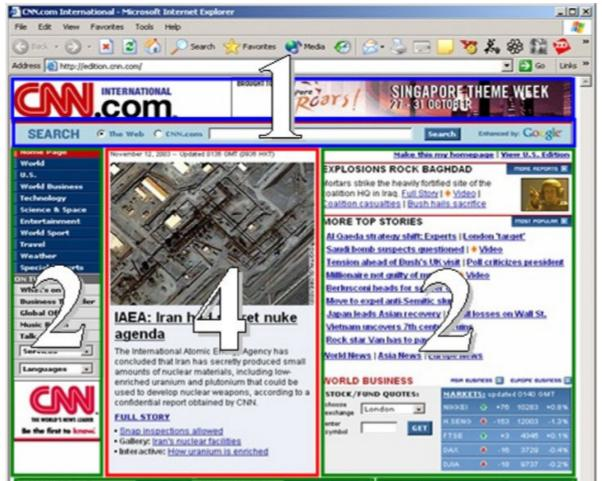
\includegraphics[scale=0.3]{cnn_rbf.jpeg}\end{center}
			\caption[Vizualizácia mapovania dôležitosti blokov webových stránok]{Vizualizácia mapovania dôležitosti blokov webových stránok\cite{block_importance}. 1 - najmenej dôležité informácie, 4 - najpodstatnejšia časť stránky}\label{fig:cnn_rbf}
		\end{figure}

	Na odhad dôležitosti blokov sa potom nahliada ako na regresný problém a na jeho riešenie je  použitá neurónová sieť, v ktorej sú bloky reprezentované ako dvojica (\textit{x, y}), kde \textit{x} je reprezentácia bloku a \textit{y} je dôležitosť (berie sa ako reálne číslo).  Typ siete je RBF (radial basis function) a vyhľadávacou technikou je štandardný gradient descent. Sieť zahŕňa 3 vrstvy, každú s inou funkciou. Prvú (vstupnú) vrstvu tvoria zdrojové uzly, druhá je jediná skrytá vrstva a zabezpečuje nonlineárnu transformáciu zo vstupného priestoru do skrytého. Obsahuje RBF neuróny, ktoré kalkulujú vstup skrytej vrstvy kombináciou vážených vstupov a odhadov. Tretia (výstupná) vrstva dodáva dôležitosť blokov do reprezentácie blokov aplikovanej v prvej (vstupnej) vrstve. 
	
	Výhodou tohto riešenia je rozdelenie stránky podľa logických blokov, nevýhodu vidím v začiatočnom ohodnotení blokov ľuďmi podľa dôležitosti, pretože mi to príde príliš individuálne. Tiež rozdelenie stránky do stromu s jednotlivými blokmi a časťami je v závislosti od stránky dosť pamäťovo náročná operácia. 
	
\subsubsection{Riešenia vychádzajúce z obrázku stránky}
\label{singapur}
	Tento typ riešenia používa k určeniu dôležitých (pútavých) častí stránky jej screenshot. Autormi modelu sú Chengyao Shen a Qi Zhao\cite{singapur_model}. Tí na začiatku rozdelili ich dataset do niekoľkých kategórií podľa obsahu stránky, t. j. ilustrované (prevládajú obrázky), textové (prevažne blogy, články, atď.) a mix predošlých dvoch kategórií. V každej z nich bolo približne 50 obrázkov s rozlíšením 1360x768. Na obrázky web stránok  potom pozeralo 11 subjektov a ich sekvencie pohľadov boli zaznamenané pomocou MATLABU s Psychtoolbox\cite{psych} a systémom Eyelink 1000.
	
	Na predikciu pohľadov\cite{saliency} na web stránky bola použitá metóda MKL (Multiple Kernel Learning - kombinuje viacero jadier SVM\footnote{Support Vector Machine - modely učenia s príslušnými algoritmami učenia, ktoré analyzujú dáta použité pre klasifikáciu a regresnú analýzu\cite{SVM}} miesto jedného). MKL bolo trénované ako binárny regresný problém, z datasetu bolo použitých 119 obrázkov na trénovanie, zvyšných 30 bolo použitých na finálne testovanie. Predikovaný bol vektor pohľadov (fixácií) na obrázok. Vyhodnotením datasetu bolo zistené, že človeka mimo iné upúta pri pohľade na web stránku v prvom rade ľudská tvár, oči a celkovo horná časť tela, či neprimerane veľké logo. Taktiež sa dá predpovedať, že človek sa začne pozerať v prvom rade najprv do strednej  oblasti a oblasti viac vľavo hore od stredu. Tieto zistenia dokázali veľmi dobre zapracovať aj do ich modelu. Na obrázku nižšie je možné vidieť vizualizáciu pohľadu na rôzne typy stránok v prvých 5 sekundách formou teplotných máp.
		\begin{figure}[H]
			\begin{center}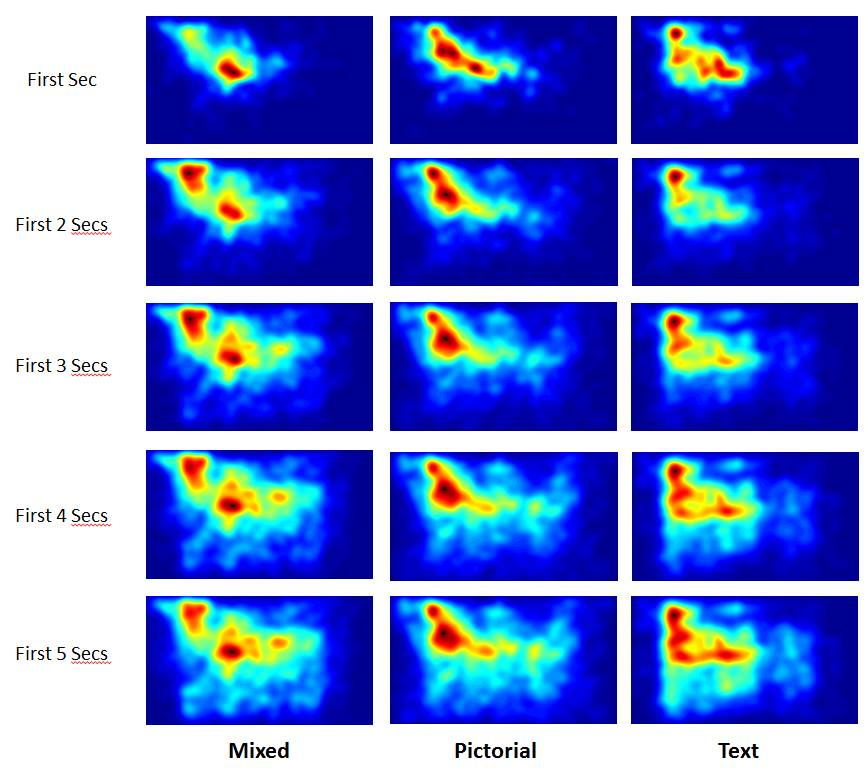
\includegraphics[scale=0.3]{heatmaps.png}\end{center}
			\caption[Vizualizácia pohľadu formou teplotných máp]{Vizualizácia pohľadov v prvých 5 sekundách. Vľavo mix stránok, v strede prevažne ilustrované stránky a vpravo textové.\cite{singapur_model}}%\label{simple_nn}
		\end{figure}
		
	Za výhodu tohto riešenia oproti predošlému pokladám hlavne vygenerovanie heat mapy, ktorá vypovie o dôležitých častiach stránky ďaleko viac ako očíslované HTML bloky. Taktiež zistenia, že človek si ako prvé všíma napríklad ľudské tváre, sú pre dizajnéra web stránky určite velké plus oproti dôležitosti informácií na základe ich umiestnenia. 
\fi

%%
%% design
%%
 \cleardoublepage
 \newpage
\newpage
\ifthenelse {\boolean{bachelor}}
{
	%\section{Design}
	\section{Návrh}
}
{
	%\chapter{Design}
	\chapter{Návrh}
}

\subsection{Prvotné experimenty}

\subsection{Návrh neurónovej siete}
\label{navrh}
\iffalse
K predikcii pohľadov na webové stránky je vhodné použiť konvolučnú neurónovú sieť, keďže webstránky sú vo forme obrázkov. Neurónová sieť bude predikovať priamo výslednú teplotnú mapu pohľadov (mapu výraznosti). Sieť by mala pozostávať z konvolučnej a združovacej vrstvy (vrstiev) pre spracovanie obrázku, nasledovaných normalizačnou vrstvou, plne prepojenou vrstvou a vrstvou výpadku (z angl. dropout layer). Za nimi nasleduje už len výstupná vrstva. Ako aktivačnú funkciu sme vybrali sigmoid, nakoľko sa bude predikovať mapa výraznosti, t. j. v podstate pravdepodobnosť pohľadu. 
\fi 
Celá architektúra je načrtnutá na schéme na obrázku \ref{my_tensorboard_cnn} vytvorenej pomocou nástroja  TensorBoard\footnote{https://www.tensorflow.org/get\_started/summaries\_and\_tensorboard/}.


\begin{figure}[H]
	\begin{center}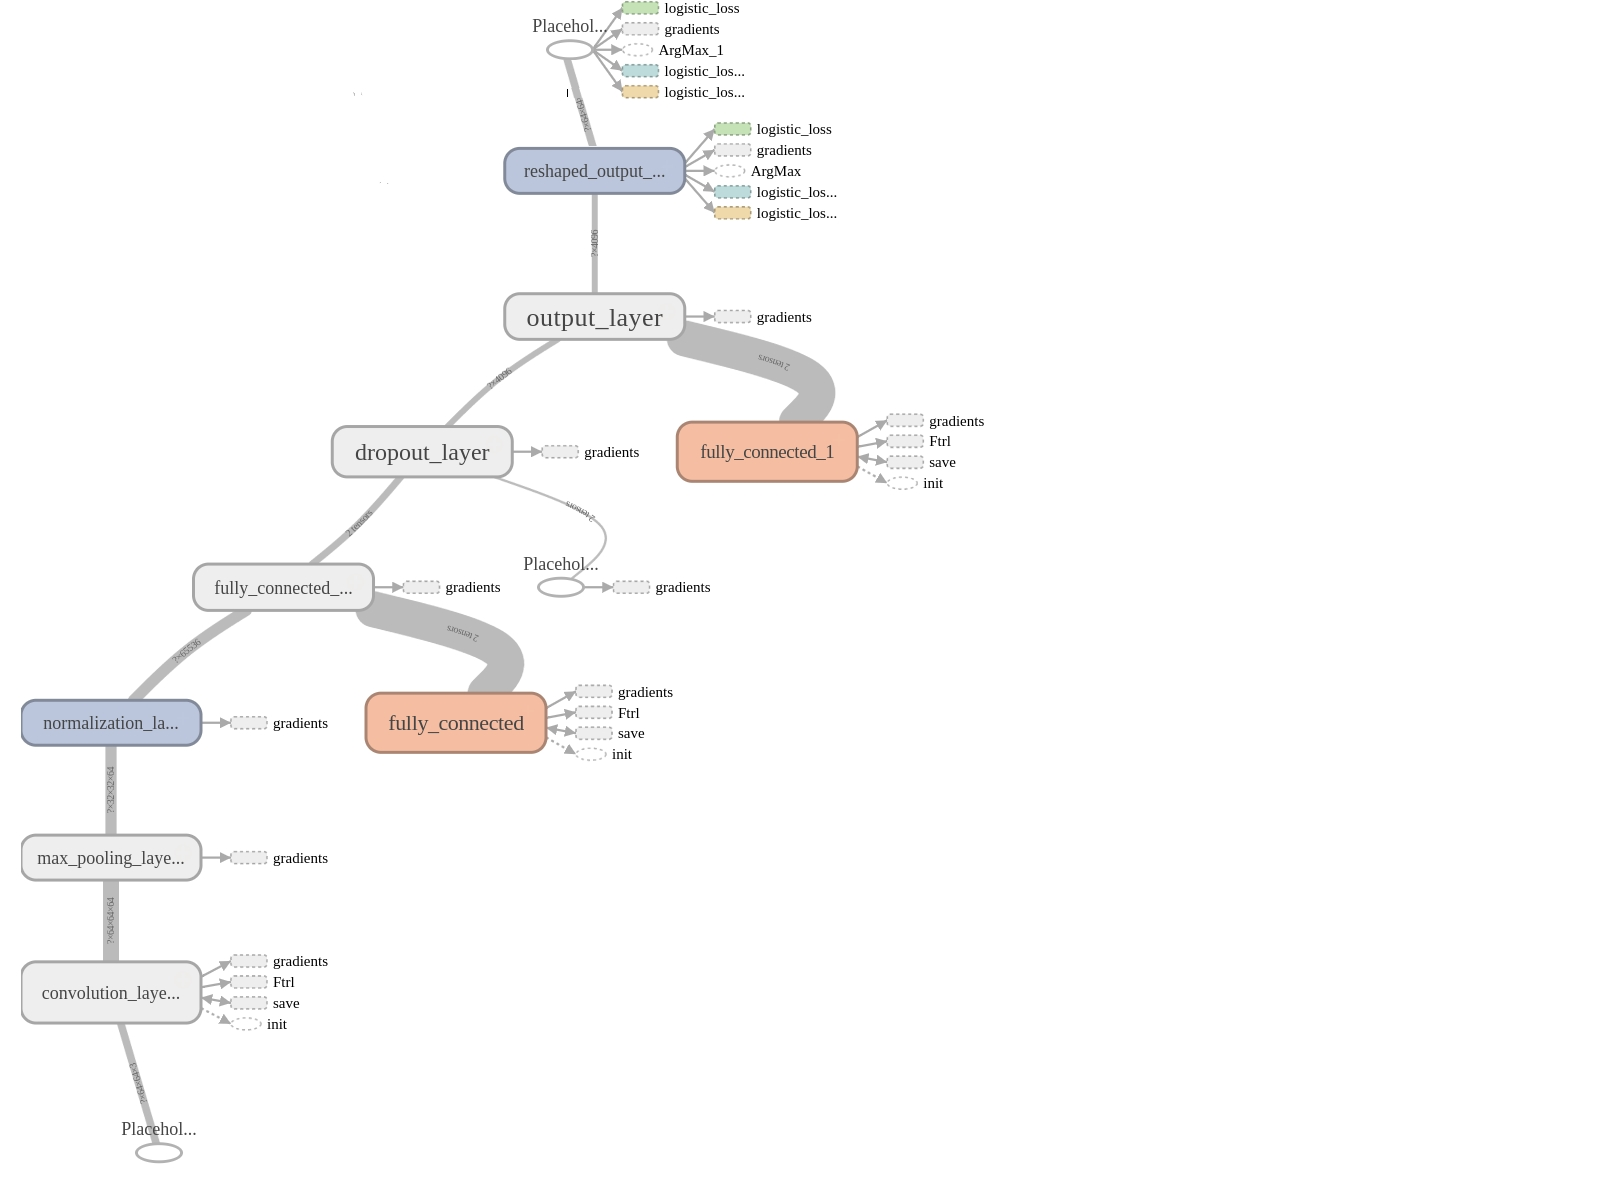
\includegraphics[scale=0.4]{graph-run.jpg}
		\caption[Návrh neurónovej siete]{
			Grafická schéma neurónovej siete, zdola vstup, vrstvy neurónovej siete, výstup (predikovaná mapa výraznosti)
		}\label{my_tensorboard_cnn}
	\end{center}
\end{figure}
\iffalse
Na konvolučnej vrstve sa použije konvolučný filter o veľkosti 5x5, ktorým sa prejde vstupný obrázok. Výstupom z nej budú mapy (obrázky) po aplikovaní filtra. Tieto dáta budú spracovávané vo vrstve združovania s použitím operácie MAX, okna (filtra) s veľkosťou 2x2 a posunom s veľkosťou 2. Výstup všetkých filtrov je zlúčený do jednej širokej vrstvy a to normalizačnej. Z nej nasledujú prepojenia do plne prepojenej vrstvy, za ktorou nasleduje vrstva výpadku\cite{dropout}. Tá prakticky obsahuje hodnotu (od 0 do 1) určujúcu koľko neurónov bude dočasne „odstránených“ z modelu spolu so všetkými spojeniami, ako vstupnými tak aj výstupnými. To by malo zabrániť pretrénovaniu siete. Za vrstvou výpadku nasleduje už len výstupná vrstva, ktorá je nakoniec ešte aj transformovaná do 2D matice reprezentujúcej predikovanú mapu výraznosti. 

Aktivačná funkcia sigmoid bude použitá iba na prvej konvolučnej vrstve a na plne prepojenej vrstve. K trénovaniu sa použije FTRL optimizér spolu s náhodným generátorom dát, ktorý bude z datasetu určenému pre fázu trénovania náhodne vyberať dáta na učenie. Tým sa zabezpečí simulácia náhodnosti vstupných dát a teda sa sieť bude schopná lepšie učiť. 
\fi 

\subsection{Dataset}
\label{dataset}
	

\iffalse
\begin{equation}
content...
\end{equation}
\fi
 \cleardoublepage
 \newpage
%\newpage

\section{Implementácia}
\label{implement}
Zdrojový kód môjho riešenia je napísaný v jazyku Python s použitím nasledujúcich hlavných knižníc:
\begin{itemize}
	\item TensorFlow\footnote{https://www.tensorflow.org/} - open-source knižnica pre strojové učenie. Použitá na vytvorenie modelu neurónovej siete a prácu s ňou.
	\item Matplotlib\footnote{https://matplotlib.org/} - knižnica pre 2D vykresľovanie. V mojom riešení je použitá hlavne na výsledné zobrazenie (resp. uloženie) predikovaných máp výraznosti (teplotných máp) na konkrétnom obrázku webovej stránky. 
	\item PIL (Python Image Library\footnote{http://www.pythonware.com/products/pil/}) - knižnica pre prácu s obrázkami. Použitá je hlavne na načítanie obrázkov webových stránok a zmenu ich rozmerov podľa potreby. 
\end{itemize}

Celá implementácia aj spolu s ukážkami zdrojových kódov funkcií je ešte podrobnejšie popísaná v prílohe \ref{technical_documentation}.

\subsection{Spracovanie datasetu pre neurónovú sieť}

Získaný dataset pozostával z 50 obrázkov a pohľadov 20 ľudí na ne. Najprv ho  bolo nutné upraviť k trénovaniu neurónovej siete. Úprava pozostávala zo zmenšenia a zmeny rozlíšenia obrázkov web stránok pre neurónovú sieť na štvorec o veľkosti \textit{a} x \textit{a}. To zabezpečuje funkcia \textit{\textbf{resize\_image (image, size)}}, ktorá ako parametre dostane obrázok a veľkosť (\textit{size = a}), na ktorú má byť obrázok prevedený.

Ďalej bola nutná normalizácia a vyfiltrovanie fixácií, k čomu slúži funkcia \textit{\textbf{load\_fixations (path)}}. Ako argument dostane CSV súbor exportovaných dát z experimentu, ktorý má za úlohu spracovať. Súbor je spracovávaný sekvenčne po riadkoch, pri čom sú ignorované pre nás nepodstatné záznamy, ako napr. pohľady na medzisnímku pre rozhodenie pozornosti. Fixácie mimo obrázka sú rovnako preskočené a každá fixácia je znormalizovaná. Dáta (meno obrázka, fixácie a ich dĺžky) sú potom uložené pre participantov jednotlivo. 

Pre neurónovú sieť je ešte nutné vypočítať mapy výraznosti (teplotné mapy) z vyfiltrovaných fixácií použítím Gaussovho rozdelenia, ktorého rovnica je ukázaná vo vzorci \ref{gauss}. Najprv však bolo nutné prepočítať fixáciu na konkrétny pixel na obrázku, pomocou nasledujúceho vzorca:

\begin{equation}
[x, y] = [fixation\_x * a, fixation\_y * a]
\label{fixation_convert}
\end{equation}

[\textit{x, y}] - bod v obrázku

\textit{a} - veľkosť strany obrázka (keďže je štvorec)

\textit{fixation\_x} - x-ová normalizovaná súradnica fixácie

\textit{fixation\_y} - y-ová normalizovaná súradnica fixácie
\newline

Toto zabezpečilo rovnakú veľkosť obrázkov a prislúchajúcich máp výraznosti k nim. Hodnota Gaussovho rozdelenia je vypočítaná prakticky pre všetky body z fixácií. 

\begin{equation}
f (x \mid  \mu, \sigma^2 ) = \frac{1}{\sqrt {2 \sigma^2 \pi}} * e^{-\frac{(x- \mu )^2}{2\sigma^2}}
\label{gauss}
\end{equation}

\textit{x} - aktuálny bod, pre ktorý je počítané Gaussovo rozdelenie

\((x - \mu )^{2}\) - vzdialenosť medzi bodom a fixáciou

\(\sigma^2\) - dĺžka fixácie
\newline

Obe vyššie uvedené matematické operácie zobrazuje časť kódu na obrázku \ref{fig:fix_gauss_code}.

	\begin{figure}[H]
		
		\begin{center}
			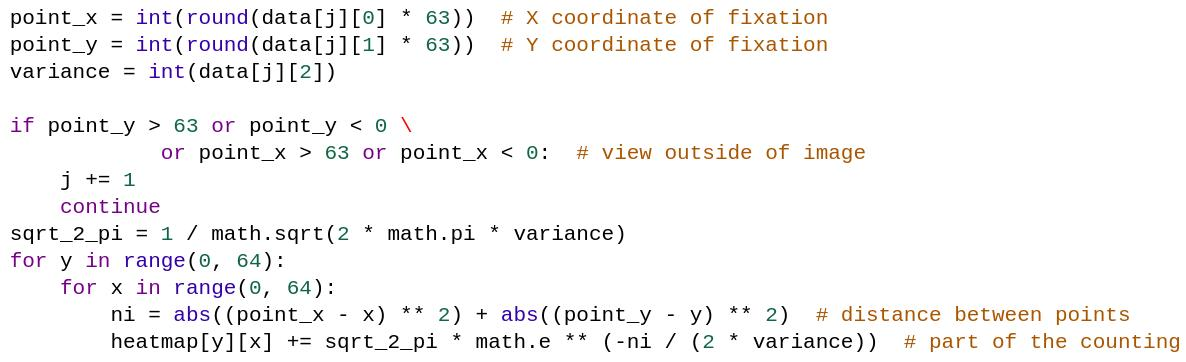
\includegraphics[scale=0.33]{fixations+gauss.jpeg}
		\end{center}
		\caption[Ukážka výpočtu heatmapy]{Ukážka výpočtu heatmapy, kde premenná data obsahuje fixácie a ich dĺžky pre všetky obrázky, heatmap je už konkrétna mapa výraznosti pre obrázok web stránky}
		\label{fig:fix_gauss_code}
	\end{figure}

Kód je súčasťou funkcie \textit{\textbf{load\_coordinates\_for\_image (file\_with\_coordinates, path)}}, ktorej prvý parametrom je súbor s fixáciami participanta a druhým je adresár (cesta) kde sa majú uložiť vypočítané heatmapy. Heatmapy sú ukladané v tvare \textit{heatmap\_i\_image\_j}, kde \textit{i} reprezentuje číslo participanta (začína od nula) a \textit{j} reprezentuje číslo obrázka (od 0 do 49). 

Takto pripravený dataset máp výraznosti pre neurónovú sieť je neskôr rozdelený v pomere 80-10-10 (trénovanie-validácia-testovanie).

\subsection{Trénovanie neurónovej siete}

Trénovanie neurónovej siete prebieha na už spomínaných 80\% dát z datasetu, 10\% je venovaných validácii. Najprv je pomocou funkcie \textit{\textbf{neural\_network\_model (data, keep\_prob)}} vytvorený model siete, ktorého schéma aj s popisom je v Návrhu v časti \ref{navrh}. Parameter \textit{data} predstavuje vstup pre neurónovú sieť, v našom prípade obrázok, resp. obrázky. Parameter \textit{keep\_prob} určuje hodnotu na vrstve výpadku (z angl. dropout layer), tá je pri trénovaní 0.5, pri validácii a testovaní 1.0. 

Po rozdelení datasetu, nastavení krížových entropií (z angl. cross entropy) a optimizéru je neurónová sieť trénovaná v 15 iteráciách po 30 epoch. V každej iterácii sa trénuje a validuje na celom datasete k tomu určenom, ten je však vždy na začiatku náhodne zamiešaný (ako je vidieť v ukážke kódu na obrázku \ref{fig:shuffle_dataset}), neurónová sieť sa teda učí na náhodných dátach a nie vždy na úplne tých istých.  

	\begin{figure}[H]
		
		\begin{center}
			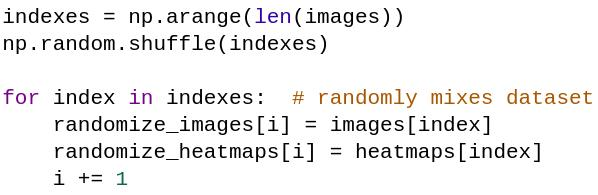
\includegraphics[scale=0.33]{random_dataset.jpeg}
		\end{center}
		\caption[Ukážka náhodného zamiešania datasetu pre trénovanie]{Ukážka náhodného zamiešania datasetu pre trénovanie}\label{fig:shuffle_dataset}
	\end{figure}
	
Vstupom do neurónovej siete je teda séria obrázkov, konkrétne o veľkosti \textit{64x64}. Výstupom sú heatmapy (mapy výraznosti) rovnakej veľkosti. 
	

Trénovanie končí buď po uplynutí všetkých epoch alebo v momente, kedy chyba predikcie na validačnom datasete prestane klesať a začne rásť. To značí, že sieť sa už neučí, ale začína sa pretrénovávať. 

Po tomto bode nasleduje otestovanie neurónovej siete na zvyšných 10\% datasetu a uloženie celého natrénovaného modelu. 

\subsection{Využívanie natrénovaného modelu}
Predikovať heatmapy k novým obrázkom pomocou natrénovaného modelu umožňuje funkcia \ \textit{\textbf{predict(model, directory\_with\_images, directory\_for\_saved\_ predictions, heatmap\_type, metrics\_set=None)}}, ktorá ako parametre dostane spomínaný model, adresár s obrázkami (na ich veľkosti nezáleží), adresár kam sa majú uložiť výsledné predikcie a typ heatmapy, ktorá sa má zobraziť. Ako voliteľný parameter je zvolenie/nezvolenie výpočtu metrík ohodnocujúcich kvalitu predikcií vizuálnej pozornosti. Po predikcii máp výraznosti sa tak v závislosti od voliteľného parametra môžu volať funkcie na výpočet už spomínaných metrík, ktoré sú prevzaté z open-source-ového repozitára\footnote{https://github.com/herrlich10/saliency}. K zobrazeniu/uloženiu predikcií slúži funkcia \textit{\textbf{visualize\_heatmap (heatmap, orig, path\_for\_saving, heatmap\_type)}}, tá má ako parametre heatmapu (teda našu predikciu), originálny obrázok, pre ktorý sa robila predikcia, cestu kam sa má uložiť výsledok a nakoniec typ zobrazovanej heatmapy. 


\newpage
\section{Experimenty}

\label{experiments}
V priebehu práce bolo nutné experimentovať v naozaj veľkom množstve s najrôznejším počtom vecí od typov neurónových sietí, datasetov až po rôzne prístupy k riešeniu zadaného problému.

Prvotné experimenty vykonávané v rámci predmetu Počítačové videnie\footnote{http://vgg.fiit.stuba.sk/teaching/computer-vision/} sú zachytené v kapitole \ref{first_experiments}. Ďalšie experimenty potom prebiehali postupne s konvolučnou neurónovou sieťou (kapitola \ref{experiments_cnn}), konvolučným autoenkóderom (kapitola \ref{experiments_autoencoder}), autoenkóderom s predtrénovanou sieťou VGG16 (kapitola \ref{experiments_vgg_net}) a autoenkóderom v kombinácii s VGG16 sieťou (kapitola \ref{vgg_autoencoder_experiments}). Rozdiel pri modeloch s VGG16 sieťou je ten, že prvý spomínaný využíva VGG16 ako enkóder, v druhom je zapojená nezávisle ako samostatná časť.  Pri každom modeli sme odskúšali nespočetné množstvo rôznych konfigurácií, pre popis sme ale vybrali len tie s najlepšími výsledkami pre jednotlivé časti. V závere v kapitole \ref{results} uvádzame porovnanie modelov použitých pri experimentoch pomocou metrík a výber toho najlepšieho. 

\subsection{Implementačné prostredie}

Všetky nižšie popisované experimenty boli naimplementované v jazyku Python za použitia najrôznejších knižníc, hlavne pre prácu s obrázkami a neurónovými sieťami (bližšie popísané v prílohe \ref{technical_doc}). Najdôležitejšími knižnicami sú:
\begin{itemize}
	\item TensorFlow\footnote{https://www.tensorflow.org/} - open-source knižnica pre prácu s neurónovými sieťami a strojovým učením
	\item Keras\footnote{https://keras.io/} - vysoko úrovňová knižnica pre prácu s neurónovými sieťami, beží na nižšie úrovňovými knižnicami ako Theano či TensorFlow
	\item Matplotlib\footnote{https://matplotlib.org/} - knižnica pre 2D vykresľovanie v Python-e
	\item OpenCV\footnote{https://opencv.org/, https://pypi.org/project/opencv-python/} - open-source knižnica pre počítačové videnie a strojové učenie
	
	Trénovanie modelov v experimentoch prebiehalo na GPU.
\end{itemize}

\subsection{Prvotné experimenty}
\label{first_experiments}
Pre prvotné experimenty sme sa rozhodli zvoliť problém predikcie vizuálnej pozornosti v častiach obrázkov, konkrétne v tzv. regiónoch záujmu (z angl. regions of interest, ROIs), ktoré sme zvolili v okolí fixácií na obrázky.

\subsubsection{Úprava datasetu}
\label{dataset}

V tejto fáze prvotných experimentov sme pracovali s datasetom zloženým z niekoľkých voľne dostupných dataset-ov vizuálnej pozornosti (CAT2000\cite{borji2015cat2000}, NUSEF\footnote{http://mmas.comp.nus.edu.sg/NUSEF.html}, ...).
Keďže vo viacerých z nich chýbali úplné informácie k výpočtu máp výraznosti, rozhodli sme sa ich získať z dostupných obrázkov máp výraznosti, kedy sme ich načítali ako jednofarebný  obrázok v odtieňoch sivej (z angl. grayscale) - hodnota pixelu vtedy prakticky reprezentuje intenzitu. Ďalej sme spolu pre vstupné obrázky a mapy výraznosti extrahovali regióny záujmu, ktoré sme zvolili v okolí fixácií - vizualizácia popisovanej extrakcie je zobrazená na obrázku \ref{roi_image}. Nevyhovujúce časti datasetov (ako napr. abstraktné umienie, fraktály, cartoon obrázky, ...) boli odfiltrované.

\begin{figure}[H]
	\begin{center}
		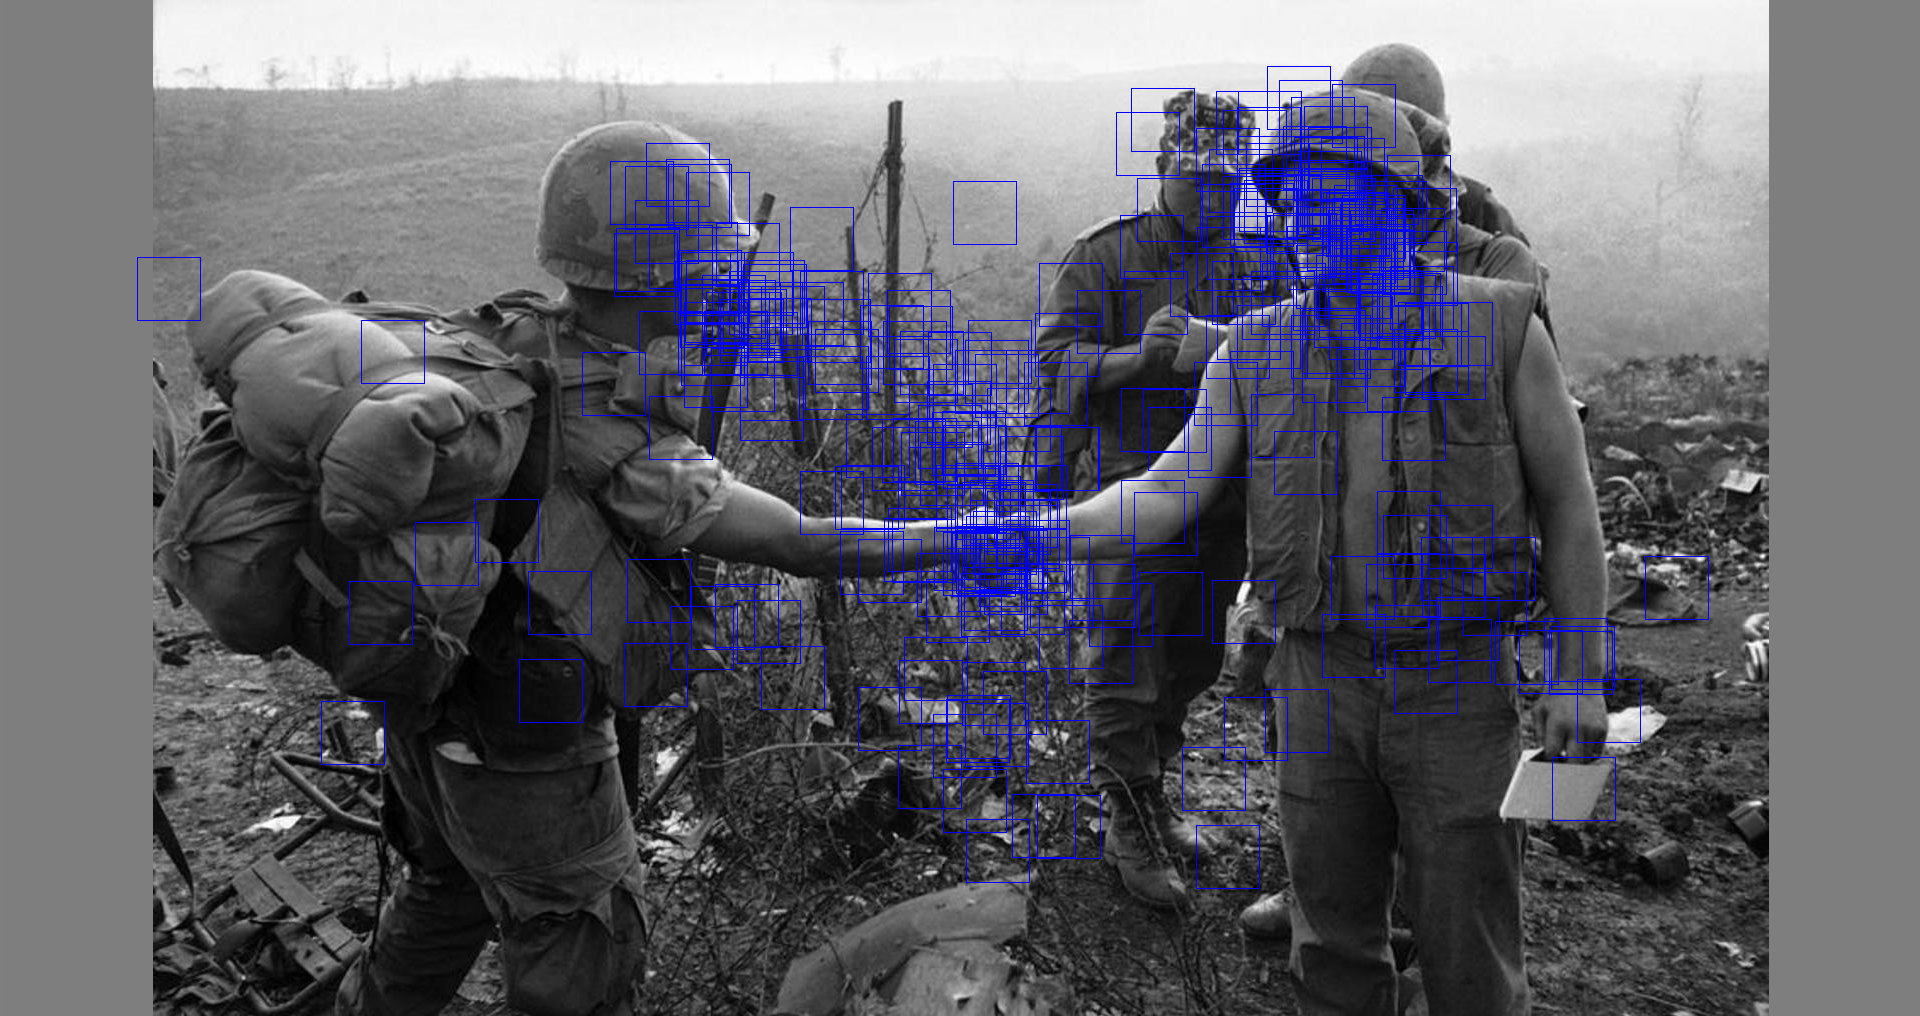
\includegraphics[scale=0.13]{img.PNG}
		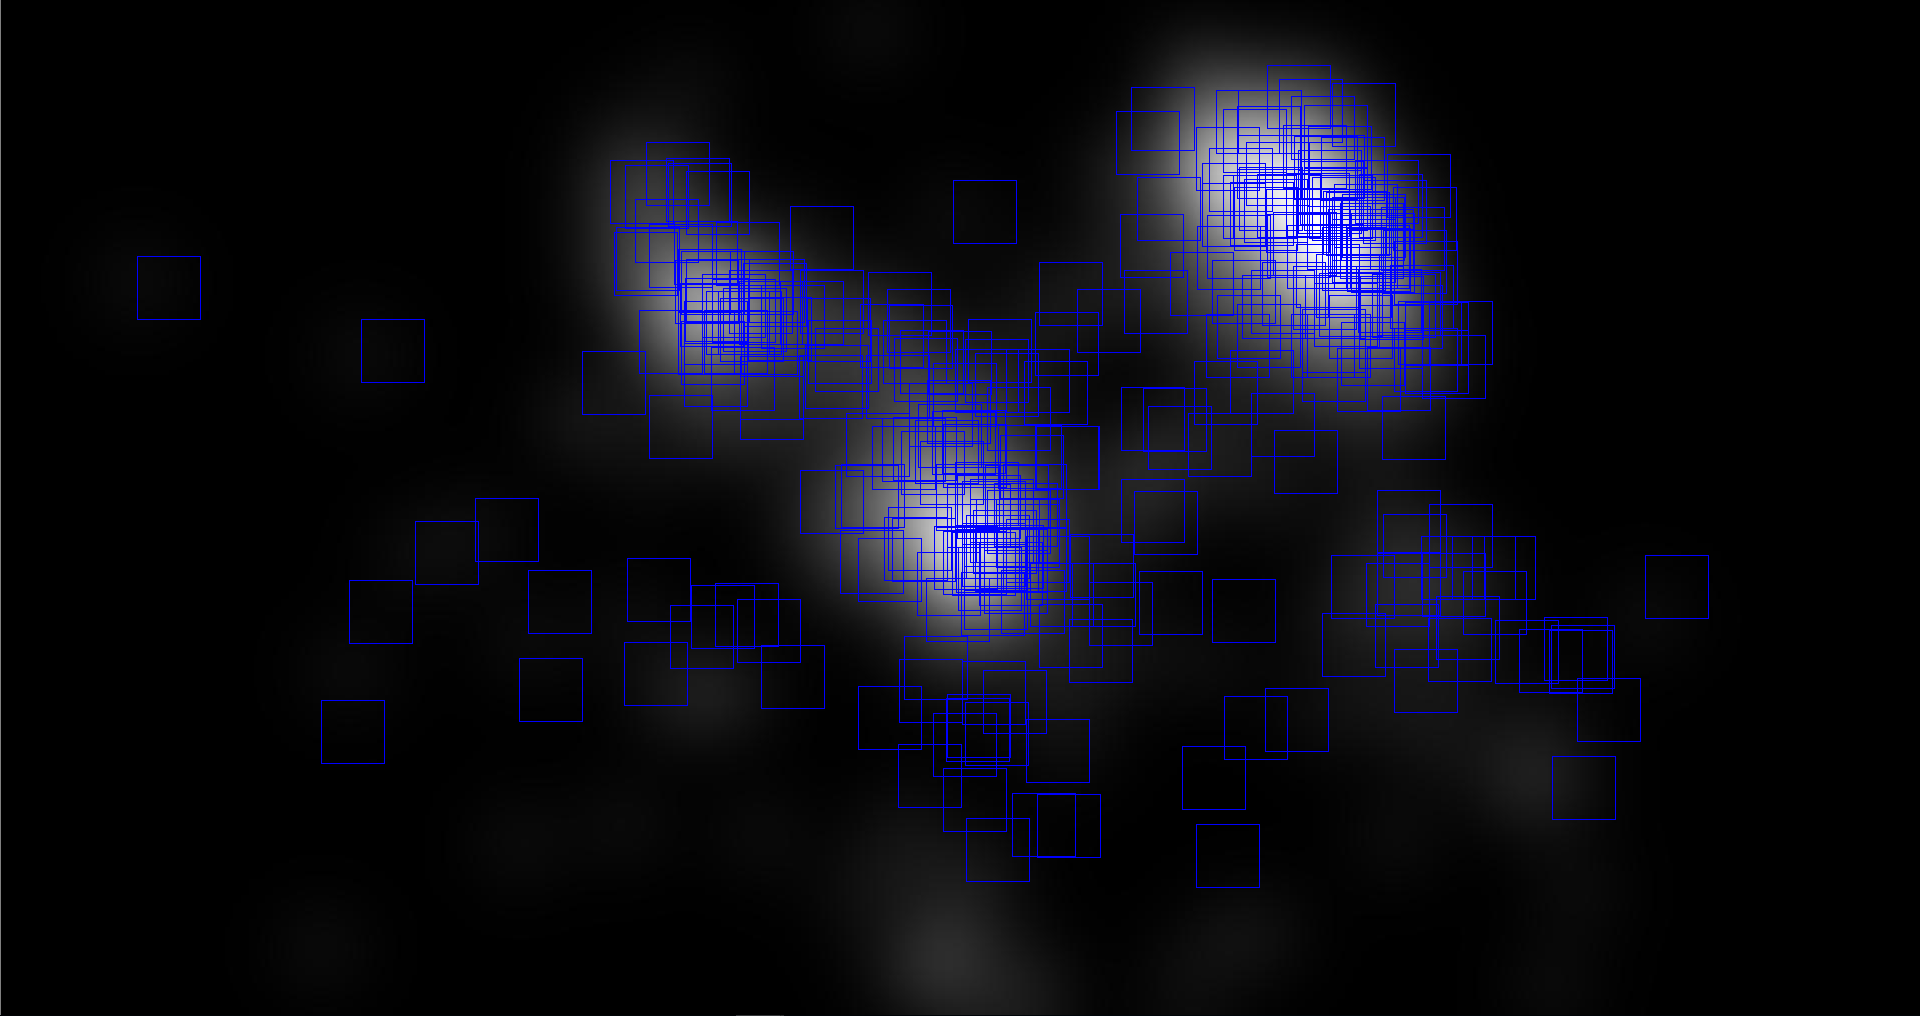
\includegraphics[scale=0.13]{map.PNG}
		\caption[Vizualizácia extrakcie regiónov záujmu]{
			Vizualizácia extrakcie regiónov záujmu, vľavo obrázok, vpravo mapa výraznosti k nemu
		}\label{roi_image}
	\end{center}
\end{figure}

Takto získané dáta boli ďalej pre neurónovú sieť normalizované, dokopy sme si nakoniec zaistili zhruba 500 000 vzoriek.
\newline

\subsubsection{Výsledky}

Navrhovanú konvolučnú neurónovú sieť (kapitola \ref{nn_popis}) sme trénovali na priravenom datasete, ktorý bol rozdelený štandardne v pomere 80:10:10 (80 - trénovanie, 10 - validácia, 10 - testovanie). Validácia prebiehala po každej iterácii a trénovanie končilo v momente keď sa chyba na validačných dátach začala výrazne odlišovať oproti najnižšej dosiahnutej (pomaly dochádzalo k pretrénovaniu). V závere mala sieť chybu predikcie na testovacích dátach na úrovni \textit{0.29}, chyba bola počítaná ako priemer chýb v každom bode obrázka. Na obrázku \ref{results_image} možno vidieť porovanie predikovaných máp výraznosti s originálnymi a so vstupnými obrázkami. 

\begin{figure}[H]
	\begin{center}
		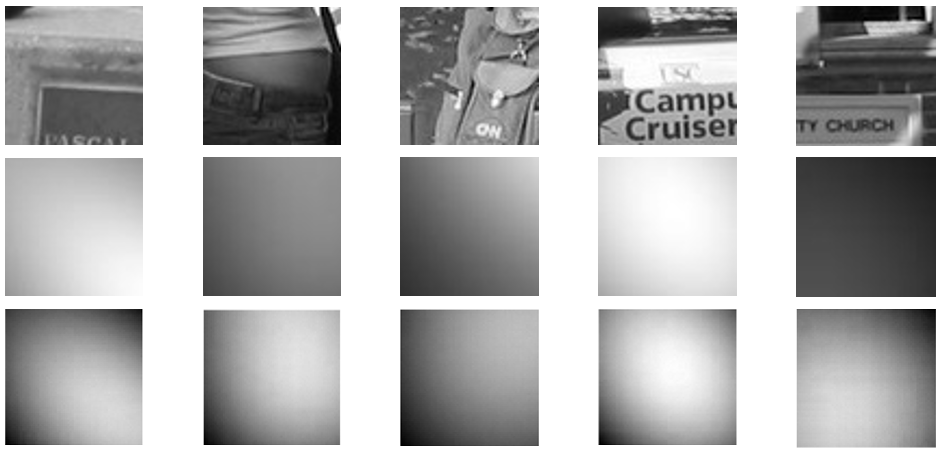
\includegraphics[scale=0.5]{predicted_saliency.PNG}
		\caption[Porovnanie prvotných výsledkov]{
			Porovnanie predikcií (dolu) s originálnymi mapami výraznosti (v strede) voči vstupným obrázkom (hore)
		}\label{results_image}
	\end{center}
\end{figure}

Pri snahe vypočítať metriky pre predikcie sme narazili na problém, ktorý sme si na začiatku neuvedomili. Väčšina metrík evaluuje mapu výraznosti voči binárnej matici reprezentujúcej fixácie na obrázok. Vzhľadom na to, že našim vstupom boli regióny záujmy v okolí fixácií, vo väčšine prípadov tieto binárne matice obsahovali len jednu fixáciu. Vďaka tomu mali metriky (AUC, sAUC, NSS) nezmyselne vysoké hodnoty. Z tohto dôvodu ich teda považujeme za nerelevantné a jediná metrika, podľa ktorej sa môžeme riadiť, je korelačný koeficient, keďže ten evaluuje predikovanú mapu voči tej pôvodnej. Jeho hodnoty na testovacích dátach sa v priemere pohybovali na hranici 0.563.

\subsection{Konvolučná neurónová sieť}
\label{experiments_cnn}

Ďalším experimentom bolo použitie klasickej konvolučnej neurónovej siete rovnako ako v predchádzajúcom prípade, tentokrát ale na celých obrázkoch. Ako dataset bol použitý spracovaný DUT-OMRON dataset (popísaný v kapitole \ref{datasets}) rozdelený podobne v pomere 80:10:10 (80 - trénovanie, 10 - validácia, 10 - testovanie), validácia bola tiež po každej epoche, trénovanie ale končilo v momente keď validačná chyba začala stúpať. Na obrázku nižšie možno vidieť vývoj jednotlivých chýb počas trénovania. Chyba bola počítaná ako priemier chýb predikcií v jednotlivých bodoch obrázka.

\begin{figure}[H]
	\begin{center}
	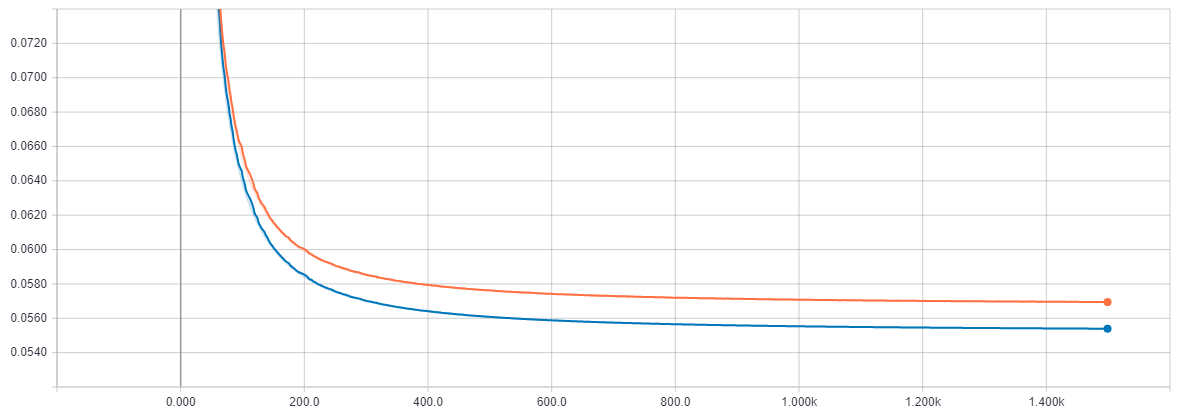
\includegraphics[scale=0.3]{nn_loss_no_outliers.png}
		\caption[Vývoj chyby počas trénovania konvolučnej neurónovej siete]{
			Graf zobrazujúci vývoj chyby neurónovej siete po odstránení extrémov počas 300 epoch - modrá farba reprezentuje chybu na trénovacích dátach, oranžová chybu na validačných dátach
		}\label{cnn_loss_outliers}
	\end{center}
\end{figure}

Z vyššie uvedených grafov vyplýva, že sieť bola schopná najvýraznejšie znížiť chybu predikcií behom prvých 50 epoch. Z jej počiatočnej hodnoty približne \textit{0.6709} klesla až na \textit{0.1321} na trénovacích dátach, na validačných dosahovala hodnotu \textit{0.1396}. Pri finálnom testovaní bola priemerná chyba približne \textit{0.1459}. Na prvý pohľad sa to môže javiť ako solídny výsledok, po vizualizovaní predikcií sme ale zistili, že sieť sa prakticky naučila predikovať ako najvýraznejšiu časť obrázka vždy len jeho stred, príklad predikcie je na obrázku \ref{cnn_results}.

\begin{figure}[H]
	\begin{center}
		
		%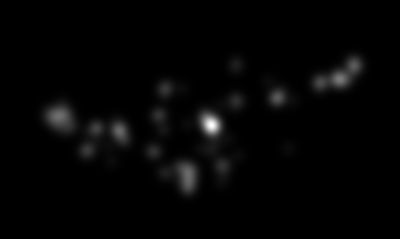
\includegraphics[width=10.58cm,height=6.32cm]{cnn_plane_heatmap.png}
		%
\includegraphics[width=10.58cm,height=6.32cm]{cnn_plane_predict.png}
		%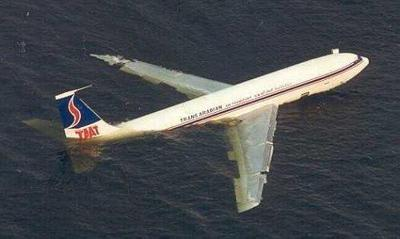
\includegraphics[width=10.58cm,height=6.32cm]{cnn_plane.png}
		%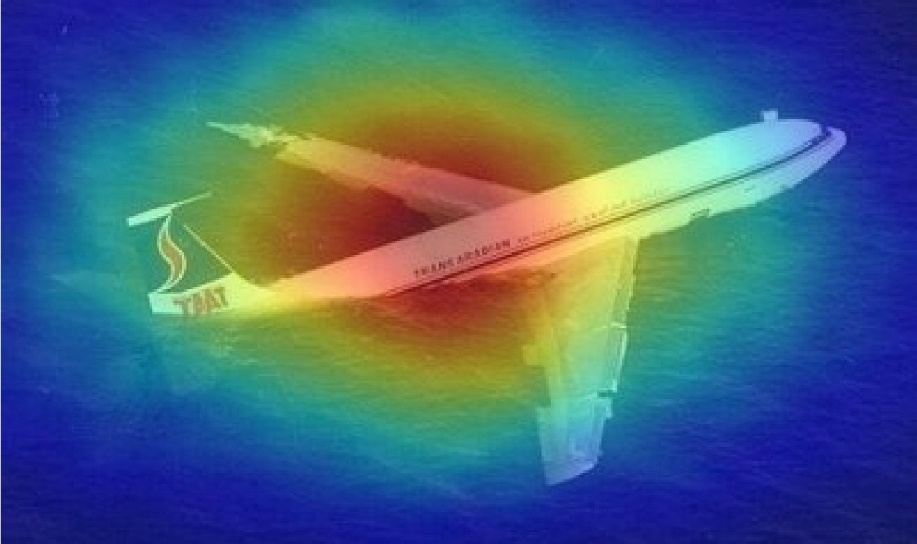
\includegraphics[width=10.58cm,height=6.32cm]{cnn_predict_on_plane.png}
		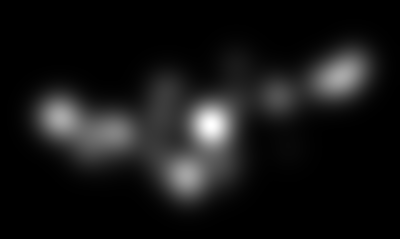
\includegraphics[scale=0.4]{cnn_plane_heatmap_regenerated.png}
		
\includegraphics[scale=0.4]{cnn_plane_predict.png}
		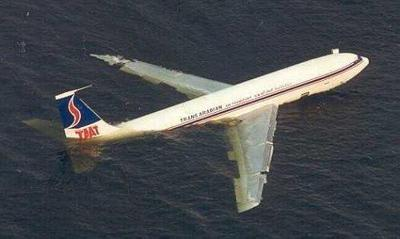
\includegraphics[scale=0.4]{cnn_plane.png}
		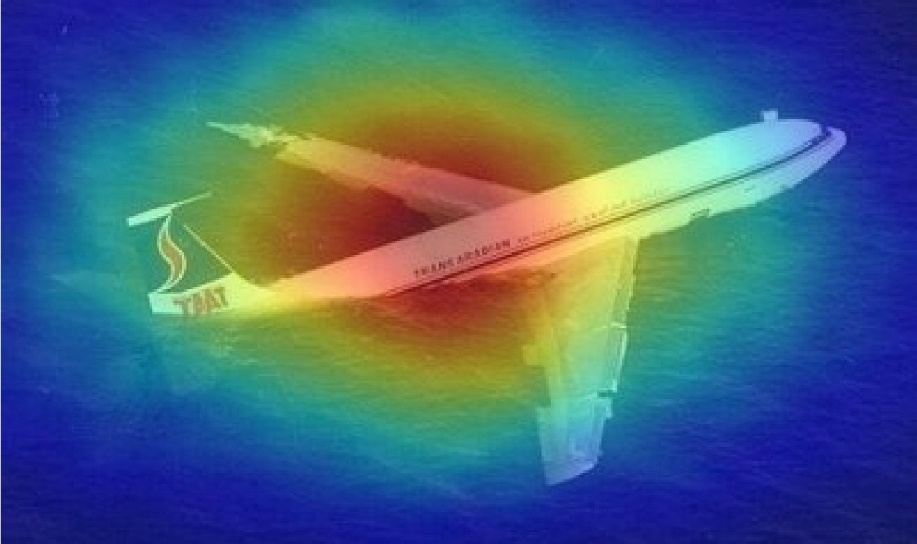
\includegraphics[scale=0.534]{cnn_predict_on_plane.png}
		\caption[Vzorka predikcie konvolučnej neurónovej siete]{
			Vľavo hore originálna mapa vizuálanej pozornosti, vpravo hore predikovaná mapa, vľavo dole obrázok pre prislúchajúce mapy výraznosti, vpravo dole zobrazenie predikcie na obrázku
		}\label{cnn_results}
	\end{center}
\end{figure}

Vyššie zobrazené správanie môže byť spôsobené napríklad relatívne malou veľkosťou vstupných obrázkov, kvôli veľkej pamäťovej náročnosti siete. 

\subsection{Konvolučný autoenkóder}
\label{experiments_autoencoder}

Ďalšou architektúrou, ktorú sme sa rozhodli vyskúšať, bol konvolučný autoenkóder (navrhnutý v kapitole \ref{autoencoder_design}). Použitý dataset bol tento krát SALICON a jeho rozdelenie bolo rovnaké ako v predošlom experimente. Trénovanie ale končilo až keď validačná chyba za posledných \textit{n} epoch neklesla. Ako funkcia chyby bola použitá priemerná absolútna chyba (z angl. mean absolute error, MAE), ktorá meria rozdiel medzi dvomi spojitými premennými, v našom prípade medzi reálnou a predikovanou mapou výraznosti, resp. ich pixelmi. Priebeh učenia možno vidieť na obrázku \ref{autoencoder_loss}. 

\begin{figure}[H]
	\begin{center}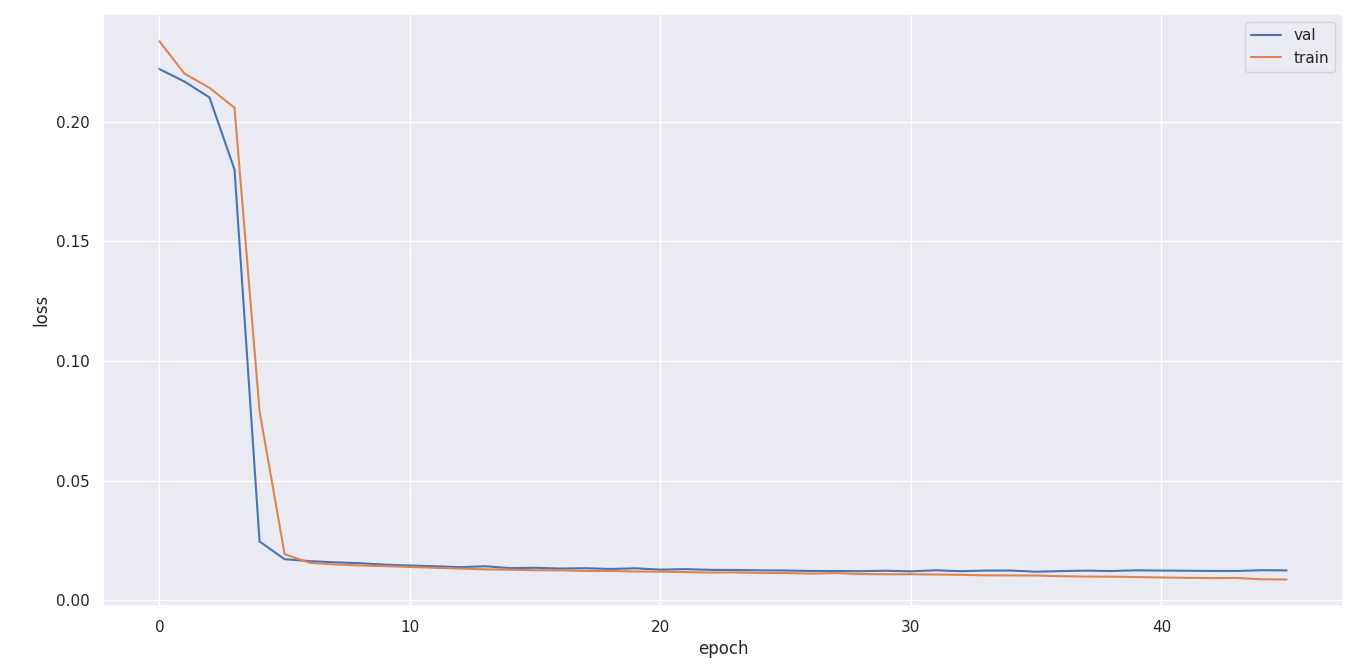
\includegraphics[scale=0.2]{autoencoder_loss.png}
		\caption[Vývoj chyby počas trénovania autoenkóderu]{
			Vývoj chyby počas trénovania, oranžovaná reprezentuje trénovaciu, modrá validačnú 
		}\label{autoencoder_loss}
	\end{center}
\end{figure}

Z obrázku je vidieť, že učenie prebiehalo počas 45 epoch, chyba najvýraznejšie klesla počas prvých šiestich epoch. Z počiatočnej hodnoty \textit{0.2336} (trénovacie dáta) a \textit{0.2219} (validačné dáta) bola schopná klesnúť až na hodnotu \textit{0.00874} (trénovacie dáta) a \textit{0.01245} (validačné dáta). Priemerná hodnota chyby pri testovaní na dátach, ktoré sieť nikdy nevidela, bola na úrovni \textit{0.01301}. Vizualizácie porovnanie predikcií sú zobrazené na obrázku \ref{autoencoder_results}.
\newpage
\begin{figure}[H]
	\begin{center}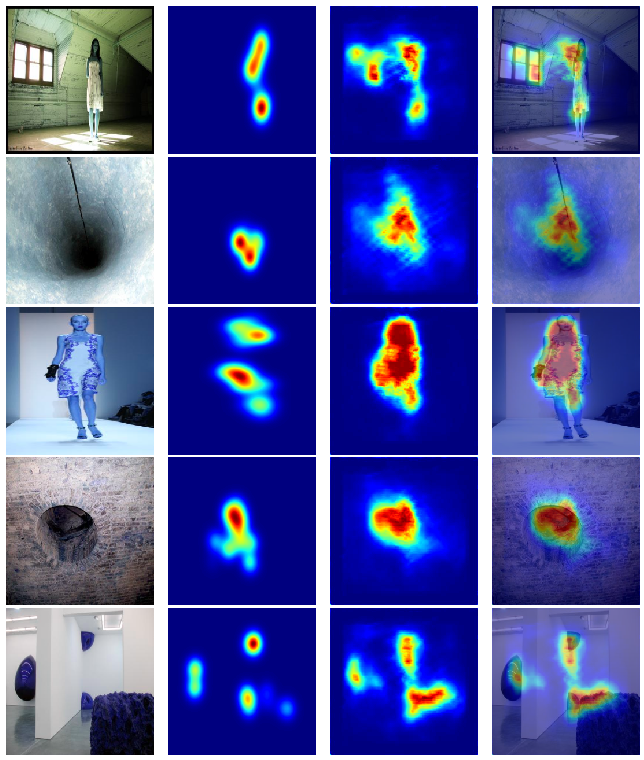
\includegraphics[scale=0.6]{autoencoder_results.png}
		\caption[Porovnanie predikcií autoenkóderu voči reálnym mapám výraznosti]{
			Porovnanie predikcií autoenkóderu, zľava vstupný obrázok, potom originálna mapa výraznosti, predikovaná mapa výraznosti a nakoniec predikcia zobrazená na obrázku. 
		}\label{autoencoder_results}
	\end{center}
\end{figure}

Z vyššie uvedených vizualizácií jasne vidieť, že sieť bola schopná naučiť sa isté výrazné súvislosti z dát, predikcie však nie sú úplne presné. Na rozdiel od siete z predošlého experimentu už nepredikuje všetko do stredu, ale je schopná označiť aj viacero výrazných objektov. To môže byť spôsobené napríklad väčšou veľkosťou vstupných obrázkov. Nakoľko autoenkóder si interne vstupné dáta zkomprimuje a zníži ich dimezionalitu, je v porovnaní zo spomínanou sieťou z predchádzajúceho experimentu pri rovnako veľkých vstupných obrázkoch menej pamäťovo náročný.

Zaujímavým javom, ktorý sme si všimli pri experimentovaní s týmto typom siete je, že hodnota chyby predikcie siete pri našom probléme nie je úplne smerodajná informácia. Pri použití napr. priemernej štvorcovej chyby (z angl. mean square error, MSE) bola výsledná chyba \textit{0.0000431}, ale predikcie boli v podstate len prázdne mapy bez akýchkoľvek výrazných častí. Tiež pri použití ešte väčšieho množstva konvolučných vrstiev sa použitá priemerná absolútna chyba zmenšila počas trénovania viac, avšak sieť sa v tomto prípade naučila predikovať najviac výrazné časti obrázkov vždy len do stredu, podobne ako pri konvolučnej neurónovej sieti z predošlého experimentu. Práve preto sme kvalitu modelov a predikcií vyhodnocovali metrikami vizuálnej pozornosti (kapitola \ref{metric}), ktorých prehľadné porovnanie aj so závermi je uvedené v \ref{results}.

\subsection{Autoenkóder s predtrénovaným modelom VGG16}
\label{experiments_vgg_net}

Pre tento experiment sme si vybrali sieť od A. Meyer-a\footnote{https://github.com/arthurmeyer/Saliency\_Detection\_Convolutional\_Autoencoder} popisovanú v kapitole \ref{object_detection}, ktorá je voľne dostupná. Jedná sa o variáciu autoenkóderu využívajúceho sieť VGG16 ako enkóder k predikcii binárnej mapy zobrazujúcej dominantné objekty v scéne. Pôvodná hypotéza bola, že vďaka použitému predtrénovanému modelu VGG16 pre detekciu objektov bude sieť lepšie rozumieť vstupný obrázkom a preto pri dodatočnom dotrénovaní k predikcii máp vizuálnej pozornosti bude dávať lepšie výsledky. Po menších úpravách siete sme pristúpili k trénovaniu na našom datasete, postupný vývoj chyby počas trénovania možno vidieť na obrázku \ref{vgg_pretrained_loss}. Validácia prebiehala každých 100 epoch, trénovanie končilo v momente keď minimálna hodnota chyby za posledných \textit{n} epoch neklesla. 
 
\begin{figure}[H]
	\begin{center}
		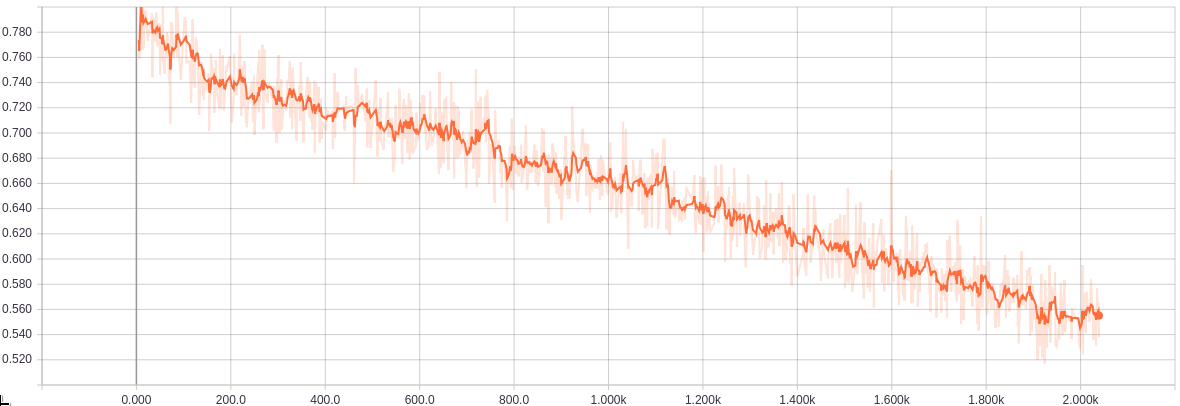
\includegraphics[scale=0.3]{vgg_pretrained.png}
		\caption[Vývoj chyby počas trénovanie siete s predtrénovaným modelom VGG16]{
			Graf zobrazujúci vývoj chyby po odstránení extrémov pri použití predtrénovaného modelu VGG16 
		}\label{vgg_pretrained_loss}
	\end{center}
\end{figure}

Na prvý pohľad sa môže zdať, že sieť sa bola schopná naučiť aspoň nejaké závislosti z dát. Po vizualizovaní dát sme ale zistili, že sme sa veľmi mýlili a snaha o dotrénovanie nepriniesla žiadne ovocie. Vizualizované výsledné dáta, ktoré mali reprezentovať mapy výraznosti, rozhodne ako mapy výraznosti nevyzerali a sieť sa nenaučila nič užitočné. Výsledkom boli len úplne náhodné hodnoty, ktoré sa ani zďaleko neblížili realite. Preto možno považovať tento experiment za nepríjemnú slepú uličku.

\subsection{Kombinácia autoenkóderu s VGG16 sieťou}
\label{vgg_autoencoder_experiments}

Hoci experiment s VGG16 sieťou použitou ako enkóder v autoenkóderi nevyšiel, stále sa nám zdalo ako dobrý nápad zapojiť do predikcií detekciu objektov. Preto sme sa pri ďalšej architektúre (kapitola \ref{vgg16_combination_with_autoencoder}) inšpirovali riešením riešením  zachytávajúcim sémantickú medzeru pri predikcii vizuálnej pozornosti (kapitola \ref{semantic_gap}). Podľa tohto návrhu sme zostrojili neurónovú sieť kombinujúcu detekciu objektov pomocou konvolučných vrstiev predtrénovanej siete VGG16 a predikciu vizuálnej pozornosti pomocou autoenkóderu. 

Sieť sme potom postupne trénovali v 2 dvoch konfiguráciach:
\begin{itemize}
	\item s vypnutím učenia pre vrstvy VGG16 siete - išlo nám o snahu zachovať kontext detekcie objektov.
	\item so zapnutím učenia pre vrstvy VGG16 siete - po odskúšaní vyššie uvedenej konfigurácie sme zistili, že mapy vizuálnej pozornosti nemajú až tak vysokú mieru granularity a chceli sme to zmeniť dotrénovaním vrstiev pre detekciu objektov. 
\end{itemize}

Na obrázku \ref{vgg16_loss_trainable_vs_nontrainable} je zobrazený vývoj  trénovacej a validačnej chyby počas učenia. Ako chyba bola zvolená binárna krížová entropia (z angl. binary cross entropy) v kombinácii s adadelta optimizérom a algoritmom spätného šírenia chyby. Učenie končilo v momente, keď sa za posledných \textit{n} epoch nezlepšila validačná chyba.

\begin{figure}[H]
	\begin{center}
		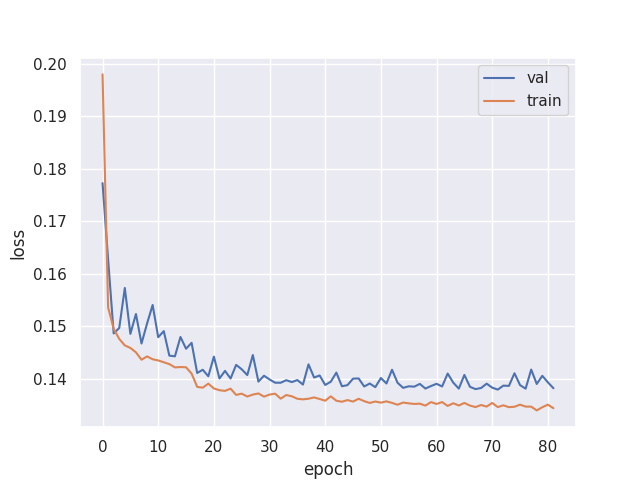
\includegraphics[scale=0.415]{vgg16_nontrainable_loss.png}
		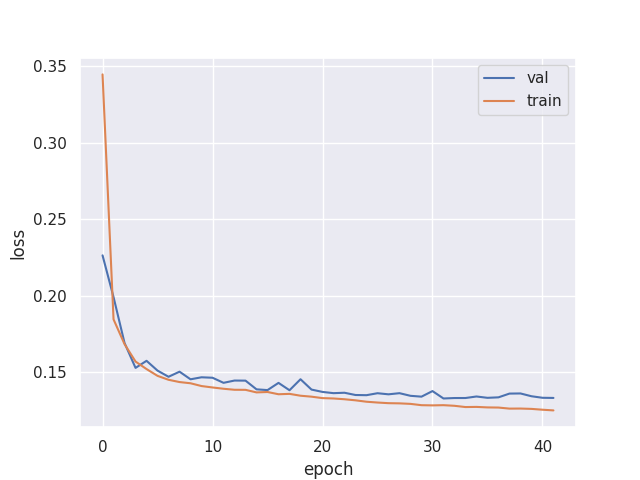
\includegraphics[scale=0.415]{vgg16_trainable_loss.png}
		\caption[Porovnanie vývoja chyby predikcie počas trénovania kombinácie autoenkóderu s VGG16 sieťou]{
			Porovnanie vývoja chyby počas trénovania, oranžová reprezentuje chybu na trénovacích dátach, modrá na validačných. Vľavo graf pre vypnuté učenie na vrstvách detekcie objektov, vpravo pre zapnuté.
		}\label{vgg16_loss_trainable_vs_nontrainable}
	\end{center}
\end{figure}

Ako je vidieť, pri zapnutom učení aj na vrstvách pre detekciu objektov (na obrázku \ref{vgg16_loss_trainable_vs_nontrainable} vpravo) bol priebeh učenia stabilnejší, kratší a aj samotná chyba bola nižšia. Jej hodnoty boli na trénovacích dátach \textit{0.125} a na validačných \textit{0.1332}, pre vypnuté učenie na vrstvách detekcie objektov (obrázok \ref{vgg16_loss_trainable_vs_nontrainable} vľavo) bola trénovacia chyba na úrovni \textit{0.1344} a validačná \textit{0.1385}. Podobne na tom bola aj chyba na testovacích dátach, a to \textit{0.1391} oproti \textit{0.1442} (so zapnutým učením menšia), čo je vzhľadom aj na takmer o polovicu menší počet epoch lepší výsledok. Na obrázkoch nižšie sú zobrazené predikcie pre jednotlivé konfigurácia spolu s porovnaním voči reálnym mapám vizuálnej pozornosti. 

% koncové hodnoty chyby: 
% nontrainable: train - 0.1344, val - 0.1382 -> 81 epoch
% trainable: train - 0.125, val - 0.1332 -> 41 epoch


\begin{figure}[H]
	\begin{center}
		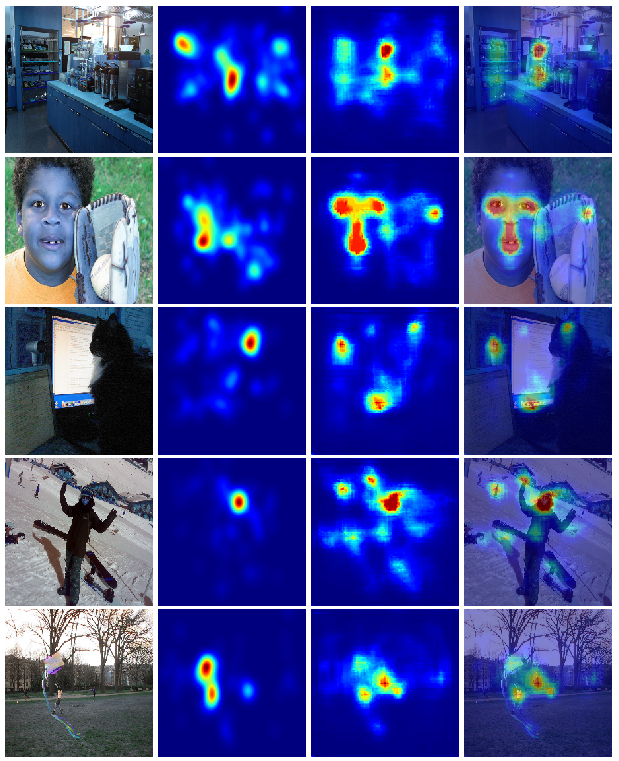
\includegraphics[scale=0.6]{vgg16_predictions_nontrainable.png}
		\caption[Porovnanie predikcií autoenkóderu s VGG16 sieťou bez dodatočného trénovania voči reálnym mapám výraznosti]{
			Porovnanie predikcií autoenkóderu s VGG16 sieťou bez zapnutého učenia, zľava vstupný obrázok, potom originálna mapa výraznosti, predikovaná mapa výraznosti a nakoniec predikcia zobrazená na obrázku.
		}\label{vgg16_predictions_nontrainable}
	\end{center}
\end{figure}

Ako je vidieť na obrázku \ref{vgg16_predictions_nontrainable}, v predikovaných mapách s vypnutým učením na vrstvách VGG16 siete cítiť vplyv detekcie objektov. Sieť vedela relatívne dobre odhadnúť salientné miesta v prípade, že na obrázku nebolo príliš veľa objektov. Problém je ale v intenzite týchto označených miest (tá býva vyššia ako v originálnych mapách) a v situáciách, kedy je na obrázku väčšie množstvo objektov. Vtedy sú v predikovanej mape vizuálnej pozornosti  označené za salientné  aj objekty, ktoré reálne nie sú (napríklad osoby v pozadí, atď.)

\begin{figure}[H]
	\begin{center}
		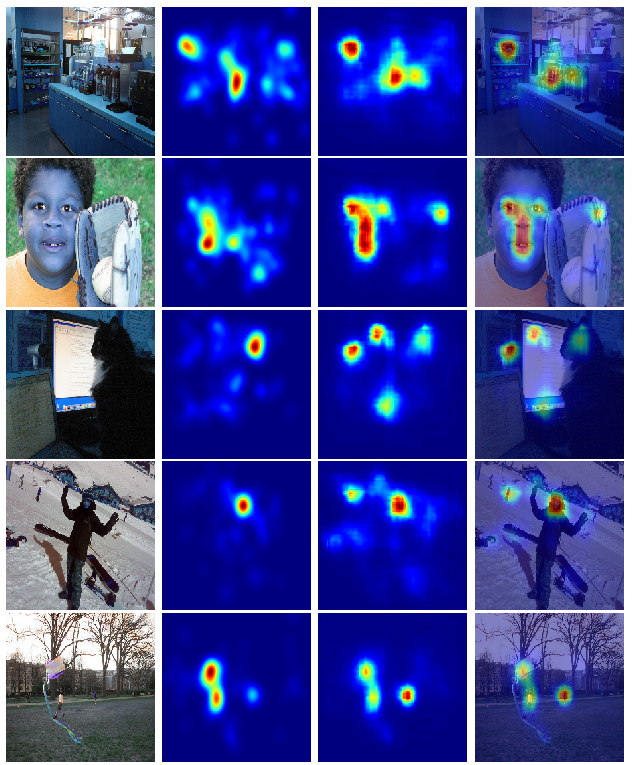
\includegraphics[scale=0.6]{vgg16_predictions_trainable.png}
		\caption[Porovnanie predikcií autoenkóderu s VGG16 sieťou s dodatočným trénovaním voči reálnym mapám výraznosti]{
			Porovnanie predikcií autoenkóderu s VGG16 sieťou so zapnutým učením, zľava vstupný obrázok, potom originálna mapa výraznosti, predikovaná mapa výraznosti a nakoniec predikcia zobrazená na obrázku.
		}\label{vgg_predictions_trainable}
	\end{center}
\end{figure}

Pri zapnutí učenia na vrstvách pre detekciu objektov sa predikcie o niečo zlepšili, sieť pri väčšom počte objektov v scéne už neoznačila tak veľké množstvo za salientné, pri čom aj predikcia intenzity v mapách je miernejšia a viac sa blíži reálnym mapám vizuálnej pozornosti. Zlepšenie koniec koncov potvrdzujú aj metriky vizuálnej pozornosti (popísané v kapitole \ref{metric}), ktorými sme ohodnotili obe konfigurácie modelu. Výsledky sú v tabuľke \ref{vgg16_trainable_vs_nontrainable_metrics}.

\begin{table}[H]
	%\begin{minipage}{\textwidth}
	\centering
	\caption[Porovnanie konfigurácií autoenkóderu s VGG16 sieťou pomocou metrík]{Porovnanie hodnôt metrík pre obe testované konfigurácie}
	\label{vgg16_trainable_vs_nontrainable_metrics}
	\begin{tabular}{{ | p{2cm} |  p{3cm} |  p{3cm} |  p{3cm} |  }}
		\hline
		& \textbf{Model s vypnutým učením pre VGG16 sieť} &  \textbf{Model so zapnutím učením pre VGG16 sieť} \\ \hline
		CC & 0.6863 & 0.8065  \\ \hline
		SIM & 0.6043 & 0.6958  \\ \hline
		AUC & 0.7678 & 0.7832  \\ \hline
		sAUC & 0.7154 & 0.7227 \\ \hline
		NSS & 1.1630 & 1.2381  \\ \hline
	\end{tabular}
	
\end{table}

\subsection{Vedená a upravená vizuálna pozornosť pri modeloch na detekciu objektov}

Ako sme popisovali v kapitole \ref{relu_and_guided_saliency}, pri natrénovaných modeloch k detekcii objektov vieme pár jednoduchými zmenami docieliť, aby sme z nich dostali salientné mapy. V rámci jedného experimentu experimentu sme teda zobrali natrénovanú VGG16 sieť, zmenili sme \textit{softmax} aktivačnú funkciu na lineárnu a postupne použili obe popísané úpravy algoritmu spätného šírenia chyby. Vizualizácie predikcií sú zobrazené na obrázkoch \ref{relu_saliency_predictions} (pre upravenú vizuálnu pozornosť) a \ref{guided_saliency_predictions} (pre vedenú vizuálnu pozornosť). 

\begin{figure}[H]
	\begin{center}
		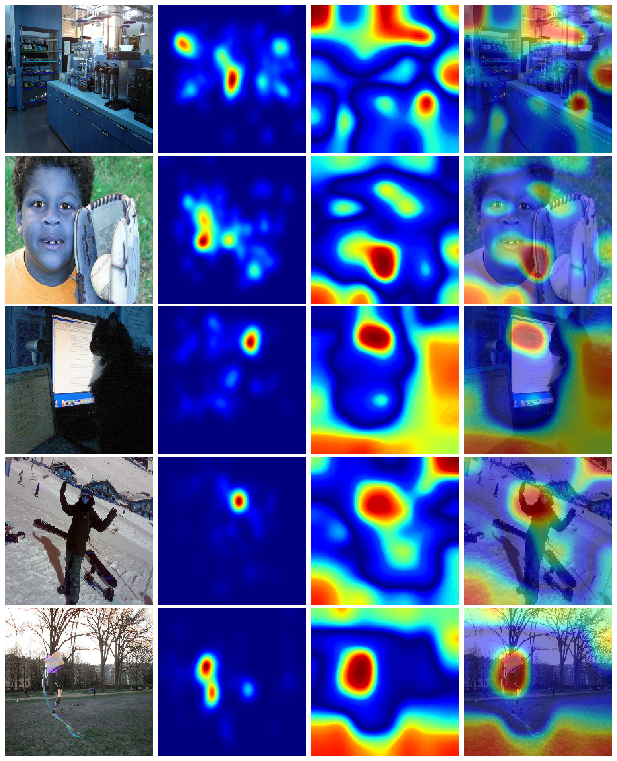
\includegraphics[scale=0.6]{relu_saliency_predictions.png}
		\caption[Porovnanie predikcií upravenej vizuálnej pozornosti voči reálnym mapám výraznosti]{
			Predikcie upravenej vizuálnej pozornosti, zľava vstupný obrázok, potom originálna mapa výraznosti, predikovaná mapa výraznosti a nakoniec predikcia zobrazená na obrázku.
		}\label{relu_saliency_predictions}
	\end{center}
\end{figure}

Vyššie zobrazené vizualizácie ukazujú, že v niektorých prípadoch sa predikcia dokázala zhruba trafiť do salientných miest, tie sú však oveľa rozsiahlejšie ako v originálnych mapách a celkovo majú predikované mapy dosť nízku granularitu. 

\begin{figure}[H]
	\begin{center}
		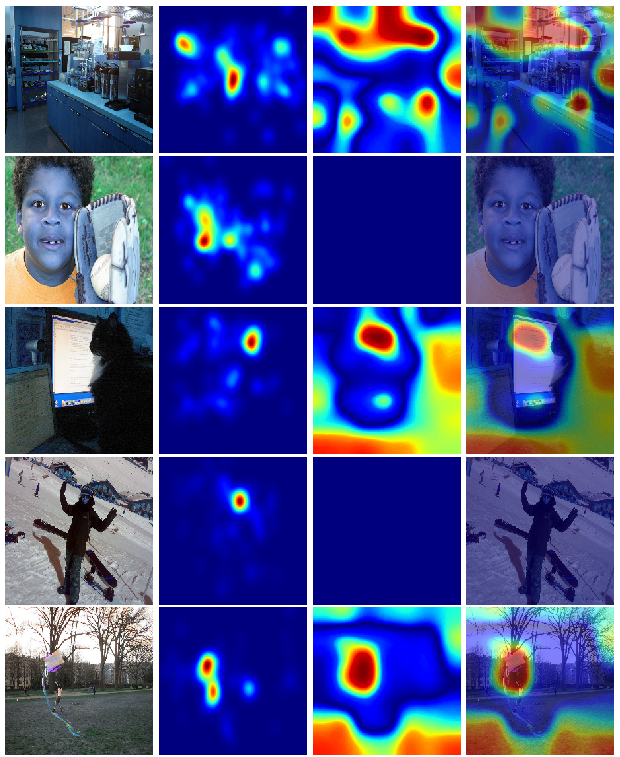
\includegraphics[scale=0.6]{guided_saliency_predictions.png}
		\caption[Porovnanie predikcií vedenej vizuálnej pozornosti voči reálnym mapám výraznosti]{
			Predikcie vedenej vizuálnej pozornosti, zľava vstupný obrázok, potom originálna mapa výraznosti, predikovaná mapa výraznosti a nakoniec predikcia zobrazená na obrázku.
		}\label{guided_saliency_predictions}
	\end{center}
\end{figure}

Pri vedenej vizuálnej pozornosti v zásade pretrvávajú podobné problémy, navyše sa však dosť často stávalo, že sme z modelu neboli schopní dostať žiadne mapy vizuálnej pozornosti. To môže súvisieť s tým, že po úprave algoritmu spätného šírenia chyby sa propaguje iba pozitívny gradient zodpovedný za pozitívne aktivácie. Celkovo predikcie nie sú veľmi presné, presnejšie ale boli mapy práve prvého typu, čo dokázali aj hodnoty metrík vizuálnej pozornosti (kapitola \ref{metric}). Ako je vidieť v tabuľke \ref{relu_vs_guided}, hodnoty metrík nedosahujú veľké čísla, rozdiely medzi dvomi typmi predikcií nie sú až tak veľké.


\begin{table}[H]
	%\begin{minipage}{\textwidth}
	\centering
	\caption[Porovnanie vedenej a upravenej vizuálnej pozornosti]{Porovnanie hodnôt metrík pre predikcie vedenej a upravnej vizuálnej pozornosti}
	\label{relu_vs_guided}
	\begin{tabular}{{ | p{2cm} |  p{3cm} |  p{3cm} |  p{3cm} |  }}
		\hline
		& \textbf{Predikcie vedenej vizuálnej pozornosti (z angl. guided saliency)} &  \textbf{Predikcie upravenej vizuálnej pozornosti (z angl. rectified saliency)} \\ \hline
		CC & 0.0259 & 0.0707  \\ \hline
		SIM & 0.2805 & 0.3040  \\ \hline
		AUC & 0.4973 & 0.5183  \\ \hline
		sAUC & 0.5018 & 0.5155 \\ \hline
		NSS & 0.0204 & 0.0763  \\ \hline
	\end{tabular}
	
\end{table}

\newpage
\subsection{Porovnanie výsledkov experimentov}
\label{results}

Do výsledného porovnania sme nakoniec zobrali iba modely s najlepšími výsledkami, pri porovnaní sme sa riadili najmä metrikami vizuálnej pozornosti, prehľadné zhrnutie ich hodnôt spolu s chybou na testovacích dátach a veľkosťou vstupných obrázkov je v tabuľke \ref{cnn_vs_autoencoder}

\begin{table}[H]

	\centering
	\caption[Porovnanie konvolučnej neurónovej siete a autoenkóderu]{Porovnanie konvolučnej neurónovej siete a autoenkóderu spolu s hodnotami metrík vizuálnej pozornosti}
	\label{cnn_vs_autoencoder}
	\begin{tabular}{{ | p{1.5cm} |  p{2.5cm} |  p{2.5cm} |  p{2.5cm} | p{2.5cm} | }}
		\hline
		& \textbf{Konvolučná neurónová sieť} &  \textbf{Autoenkóder}  &  \textbf{Kombinácia autoenkóderu s VGG16 sieťou} &  \textbf{Upravená vizuálna pozornosť} \\ \hline
		Veľkosť vstupných obrázkov & 64x64 & 256x256 & 224x224 & 224x224 \\ \hline
		Chyba na testovacích dátach & 0.1459 & 0.01301  & 0.1391 & - \\ \hline
		\textbf{Metriky} &  &  &  &  \\ \hline
		CC & 0.3891 & 0.4634 & 0.8065 & 0.0707\\ \hline
		SIM &  0.3058 & 0.3989 & 0.6958 & 0.3040\\ \hline
		AUC & 0.6892 & 0.7767 & 0.7832 & 0.5183\\ \hline
		sAUC & 0.6631 & 0.7245 & 0.7227 & 0.5155\\ \hline
		NSS & 0.7334 & 1.1288  & 1.2381 & 0.0763\\ \hline
	\end{tabular}
	
	%\end{minipage}
\end{table}

Z vyššie uvedenej tabuľky jasne vyplýva, že najlepšie výsledky má autoenkóder, resp. jeho kombinácia s VGG16 sieťou. I keď hodnoty AUC majú dosť podobné, korelačný koeficient (CC) a podobnosť (SIM), ktoré validujú predikované mapy voči reálnym, nie voči fixáciám, sú výrazne vyššie. Preto sme sa ho rozhodli ako najlepší model, ktorý sa nám podarilo vytvoriť, ďalej porovnať s už existujúcimi modelmi na viacerých datasetoch.

\section{Porovanie s existujúcimi riešeniami}
\label{compare_section}

Náš najlepší model (autoenkóder kombinovaný s VGG16 sieťou pre detekciu objektov) sme porovnali s existujúcimi riešeniami - s modelom pre redukciu sémantických medzier (kapitola \ref{semantic_gap}) a s modelom SAM (Saliency Attentive Model, kapitola \ref{sam}). Porovanie prebiehalo pomocou metrík vizuálnej pozornosti na viacerých datasetoch (popísané v kapitole \ref{datasets}). Ich výsledné hodnoty sú v tabuľke \ref{compare_solutions}.

\begin{table}[H]
	
	\centering
	\caption[Porovnanie nášho najlepšieho modelu s existujúcimi riešeniami]{Porovnanie nášho najlepšieho modelu s existujúcimi riešeniami na rôznych datasetoch pomocou metrík}
	\label{compare_solutions}
	\begin{tabular}{{ | p{1.7cm} |  p{2.5cm} |  p{2.5cm} |  p{2.5cm} | p{2.5cm} | }}
		\hline
		& \textbf{Kombinácia autoenkóderu s VGG16 sieťou} &  \textbf{Model pre redukciu sémantických medzier} &  \textbf{SAM (Saliency Attentive Model)} \\ \hline
		\textbf{Salicon} &  &  &  \\ \hline
		CC & 0.8065 & - & 0.811 \\ \hline
		SIM &  0.6958 & - & - \\ \hline
		AUC & 0.7832 & - & 0.878 \\ \hline
		sAUC & 0.7227 & - & 0.782 \\ \hline
		NSS & 1.2381 & -  & 3.15 \\ \hline
		\textbf{MIT1003} &  &  &  \\ \hline
		CC & 0.6161 & 0.74 & 0.738 \\ \hline
		SIM &  0.5075 & 0.60 & - \\ \hline
		AUC & 0.8193 & 0.85 & 0.908 \\ \hline
		sAUC & 0.7369 & 0.74 & 0.613 \\ \hline
		NSS & 1.7388 & 2.12  & 2.231 \\ \hline
		\textbf{CAT2000} &  &  &  \\ \hline
		CC & 0.7157 & - & 0.845 \\ \hline
		SIM &  0.6169 & - & - \\ \hline
		AUC & 0.8768 & - & 0.874 \\ \hline
		sAUC & 0.8237 & - & 0.539 \\ \hline
		NSS & 2.1150 & -  & 2.233 \\ \hline
	\end{tabular}
	
	%\end{minipage}
\end{table}

Pre výpočet metrík nášho riešenia sme ako základný model použili ten natrénovaný na SALICON datasete, pre ďalšie datasety (MIT1003, CAT2000) sme ho už len postupne dotrénovali. Počas trénovania aj dotrénovávania boli dáta pre každý dataset rozdelené v pomere 80 : 10 : 10 (trénovanie : validácia : test). Výsledné hodnoty metrík boli vypočítané na testovacích dátach pre jednotlivé datasety.

Ako je vidieť v predošlej tabuľke, hodnoty nášho modelu sa vo väčšine prípadov blížia hodnotám uvedených riešení, len zriedkavo sú lepšie. Naše predikcie sú teda konkurencie schopné, nie sú ale ani zďaleko najlepšie možné. 

\iffalse
MIT1003
final correlation coeficient: 0.6161522189830408
final SIM: 0.507501539429815
final NSS: 1.7388561018606992
final judd AUC: 0.8193171082796084
final shuffled AUC: 0.7369328732828082
final borji AUC: 0.7369328732828082

CAT2000
final correlation coeficient: 0.71578752863242
final SIM: 0.6169893727935132
final NSS: 2.1150046837329866
final judd AUC: 0.8768191933449266
final shuffled AUC: 0.8237329292507087
final borji AUC: 0.8237329292507087
\fi

\iffalse
cnn:

final correlation coeficient: 0.3891757367163311
final SIM: 0.30586936122666497
final NSS: 1.2774279939809017
final judd AUC: 0.8380535277085104
final shuffled AUC: 0.8247464580221275
final borji AUC: 0.8247464580221275

autoencoder:

final correlation coeficient: 0.46347693013377667
final SIM: 0.39894061994859475
final NSS: 1.1588045041398367
final judd AUC: 0.7967435191207479
final shuffled AUC: 0.7245778882530994
final borji AUC: 0.7245778882530994


\fi

%%
%% test
%%
%\newpage
\section {Výsledky}
\label{results}
V nasledujúcej kapitole sú rozobraté dosiahnuté výsledky. Na tie je nutné pozrieť sa z dvoch strán, najprv z pohľadu neurónovej siete a toho, ako dobre sa neurónová sieť dokázala naučiť predikovať na predložených dátach. Potom z pohľadu kvality predikcií a ich porovnania s inými riešeniami použitím metrík na evaluáciu modelov vizuálnej pozornosti. 

\subsection{Evaluácia modelu neurónovej siete}
\label{evaluation}
Na evaluáciu toho, ako dobre bola sieť schopná naučiť sa predikovať sme použili jednoduchý priemer chýb predikcií v jednotlivých bodoch heatmapy.
Ten potom podľa očakávania klesal počas tréningu aj validácie štandardne, ako bolo ukázané na grafoch v časti \ref{model_graph}. Jeho hodnota bola pri testovaní na testovacom datasete 0.2066. Vzhľadom na to, že pri trénovaní na 3/4 datasetu bola chyba 0.2511, predpokladáme, že ďalšie zlepšenie predikcií a zníženie chyby by bolo možné dosiahnuť väčším množstvom dát.

\subsection{Metriky používané na ohodnotenie modelov vizuálnej pozornosti}
\label{metric}
Tradične sa tieto modely evaluujú vzhľadom na pohyb očí, resp. samotné fixácie. K tomu slúži značný počet rôzne fungujúcich metrík\cite{metriky}, najpoužívanejšie sú:

\begin{itemize}

	\item NSS - Normalizovaná cesta pútavosti (z angl. Normalized Scanpath Saliency). Využíva priemer hodnôt pútavosti na \textit{n} fixácií v normalizovanej mape podľa nasledovného vzorca: 
	
	\begin{equation}
	\frac{1}{n} \sum_{i=1}^{n} \frac{s(x_{h}^{i}, y_{h}^{i}) - \mu_{s}}{\sigma _{s}}
	\end{equation}
	
	\item AUC - Oblasť pod ROC krivkou (z angl. Area Under the ROC Curve).
	Ľudské fixácie sú považované za pozitívnu sadu a niektoré body na obrázku sú vybrané ako negatívna sada. K mape pútavosti je potom pristupované ako k binárnemu klasifikátoru na separáciu pozitívnych vzorkov od negatívnych. Presnosť podľa tejto metriky je daná nasledovne: 
	
	\begin{itemize}
		
		\item 0.90 - 1 = výborná
		\item 0.80 - 0.90 = dobrá
		\item 0.70 - 0.80 = priemerná
		\item 0.60 - 0.70 = slabá
		\item 0.50 - 0.60 = veľmi slabá
		
	\end{itemize}
	
	\item sAUC - Zamiešaná oblasť pod ROC krivkou (z angl. shuffled Area Under the ROC Curve) je mierna modifikácia vyššie uvedenej metriky, kedy ako negatívna sada nie sú vybrané len niektoré body, ale všetky body, ktoré nie sú ľudskými fixáciami, sú považované za negatívne. Určenie presnosti na základe hodnôt je rovnaké ako pri AUC. 
	
	\item CC - Korelačný koeficient, určuje prakticky podobnosť v tomto prípade dvoch máp výraznosti, kde jedna je výsledok modelu vizuálnej pozornosti a druhá je reálna mapa vypočítaná z fixácií. 
	
	\begin{equation}
	CC (s, h) = \frac{cov(s, h)}{\sigma_{s} \sigma _{h}}
	\end{equation}
\end{itemize}

Z vyššie popísaných metrík sme k finálnej evaluácii a porovnaniu s inými riešeniami použili tri, a to CC, sAUC a NSS.
  
\subsection{Porovnanie s inými riešeniami}
\label{comparison}
Výsledné predikcie nášho riešenia sme porovnali s Itti-ho modelom vizuálnej pozornosti (popísaný v \ref{itti}) pomocou vyššie uvedených metrík. Metriky boli počítané na nových testovacích dátach, ktoré naša neurónová sieť doteraz nevidela. Je však nutné spomenúť, že Itti-ho model nie je primárne zameraný na určovanie vizuálne pútavých častí grafických rozhraní web stránok, jedná sa skôr o všeobecný model vizuálnej pozornosti. Porovnanie a hodnoty metrík je možné násť v tabuľke \ref{itti_vs_my}.

\begin{table}[H]
	%\begin{minipage}{\textwidth}
		\centering
		\caption[Porovnanie s Itti-ho modelom vizuálnej pozornosti]{Porovnanie hodnôt metrík pre Itti-ho a náš model}
		\label{itti_vs_my}
		\begin{tabular}{{ | p{2cm} |  p{3cm} |  p{3cm} |  p{3cm} |  }}
			\hline
			& \textbf{Itti-ho model} &  \textbf{Náš model} \\ \hline
			CC & 0.4535 & 0.6620  \\ \hline
			sAUC & 0.5785 & 0.7163 \\ \hline
			NSS & 0.3309 & 0.6998  \\ \hline
		\end{tabular}
		
	%\end{minipage}
\end{table}

Z tabuľky je vidieť, že náš model bol podľa metrík schopný predikovať o niečo presnejšie mapy výraznosti ako Itti-ho model. Na obrázku \ref{fig:itti_vs_my} je zobrazené porovnanie predikcií formou vizualizácie. 

	\begin{figure}[H]
		\begin{center}
			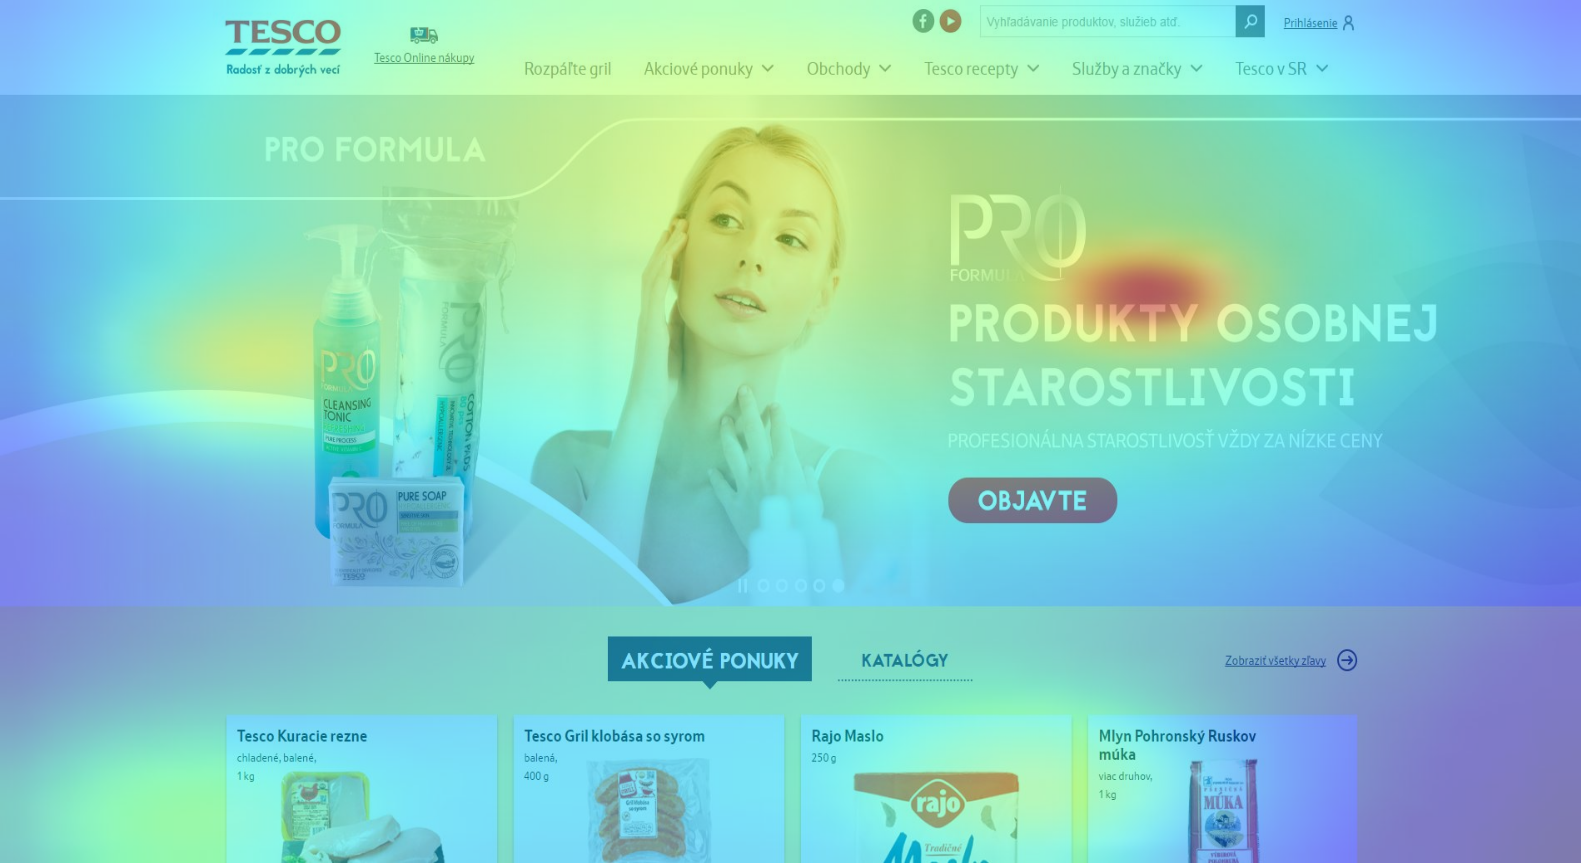
\includegraphics[scale=1, width = 4cm, height = 2.5cm]{original_2.png}
			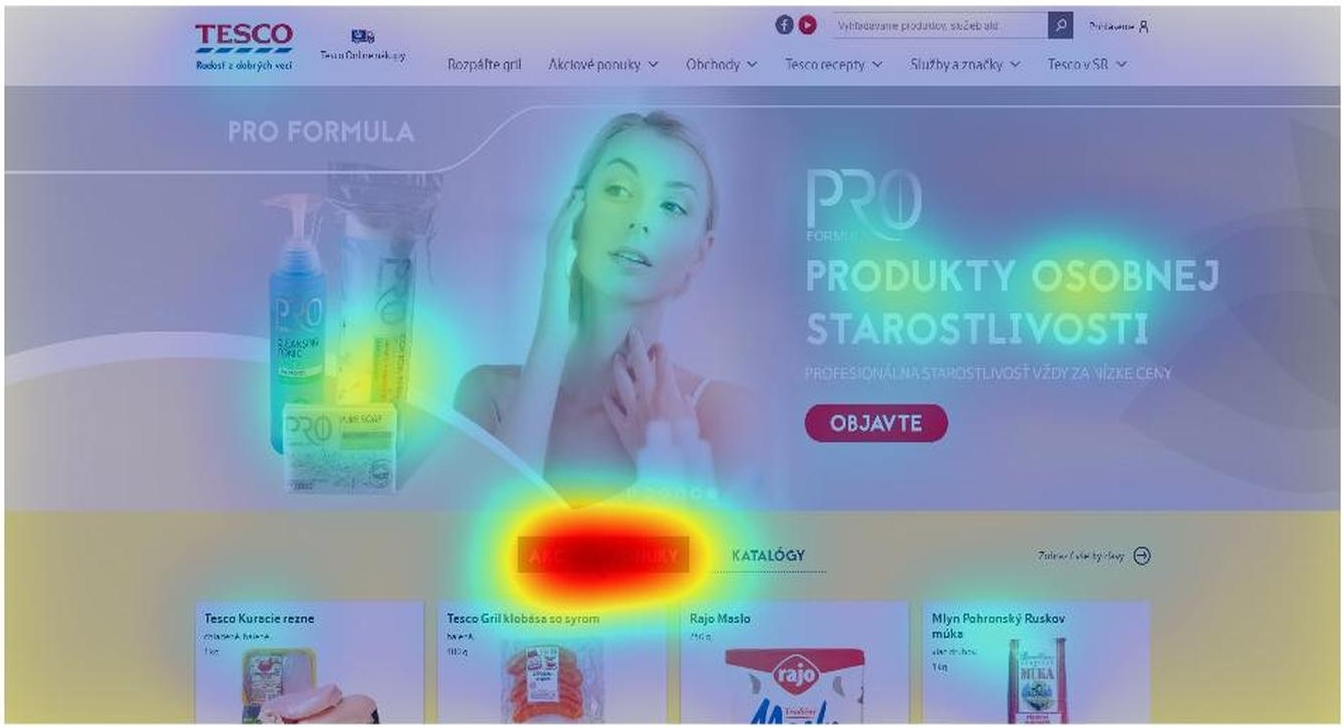
\includegraphics[scale=1, width = 4cm, height = 2.5cm]{itti_2.jpg}
			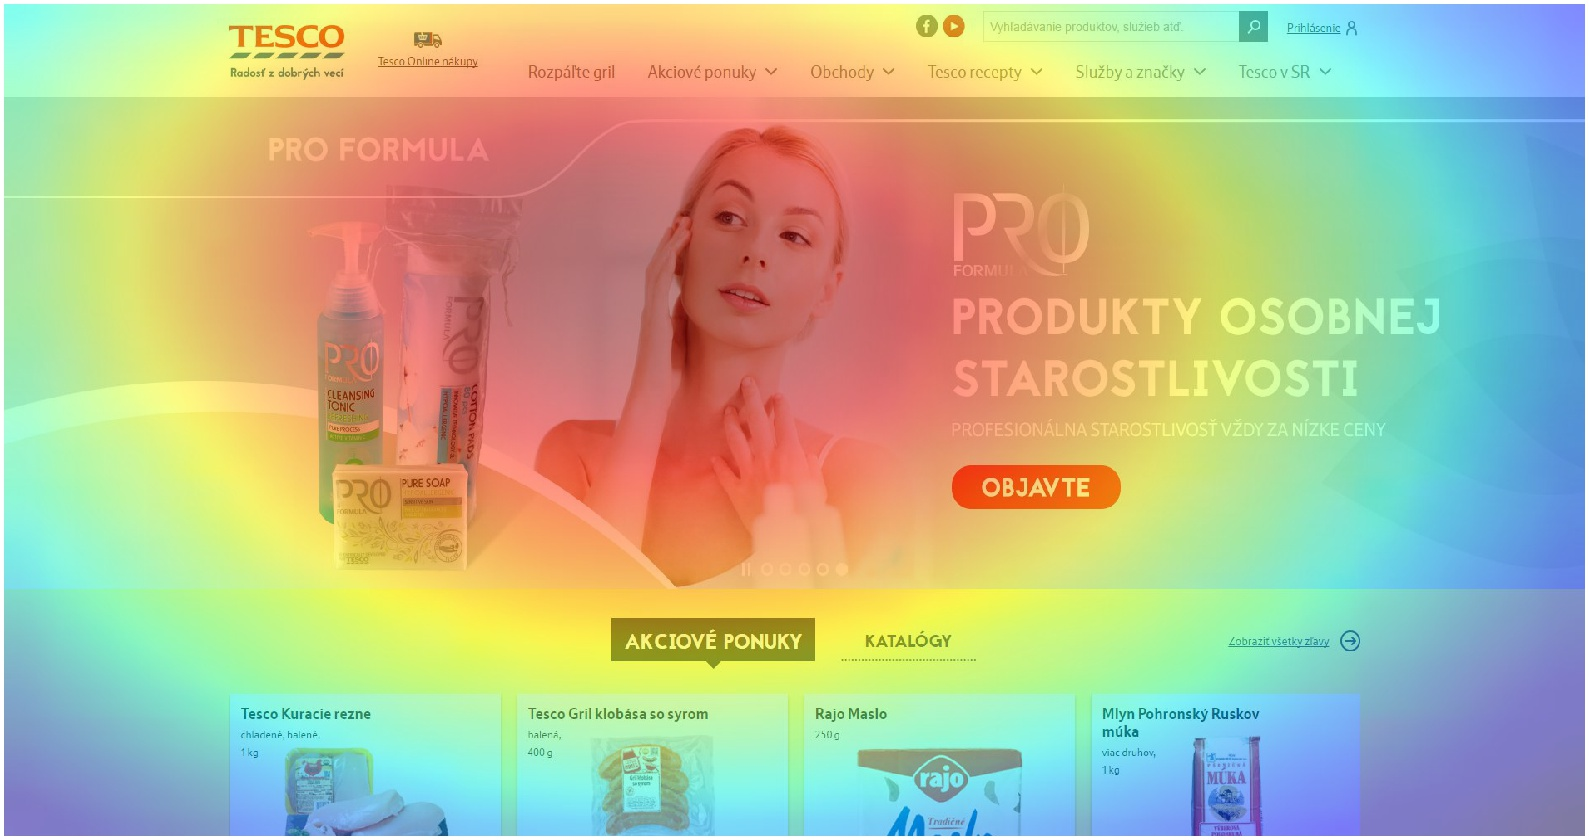
\includegraphics[scale=1, width = 4cm, height = 2.5cm]{prediction_for_tesco.jpg}			
		\end{center}
		\begin{center}
			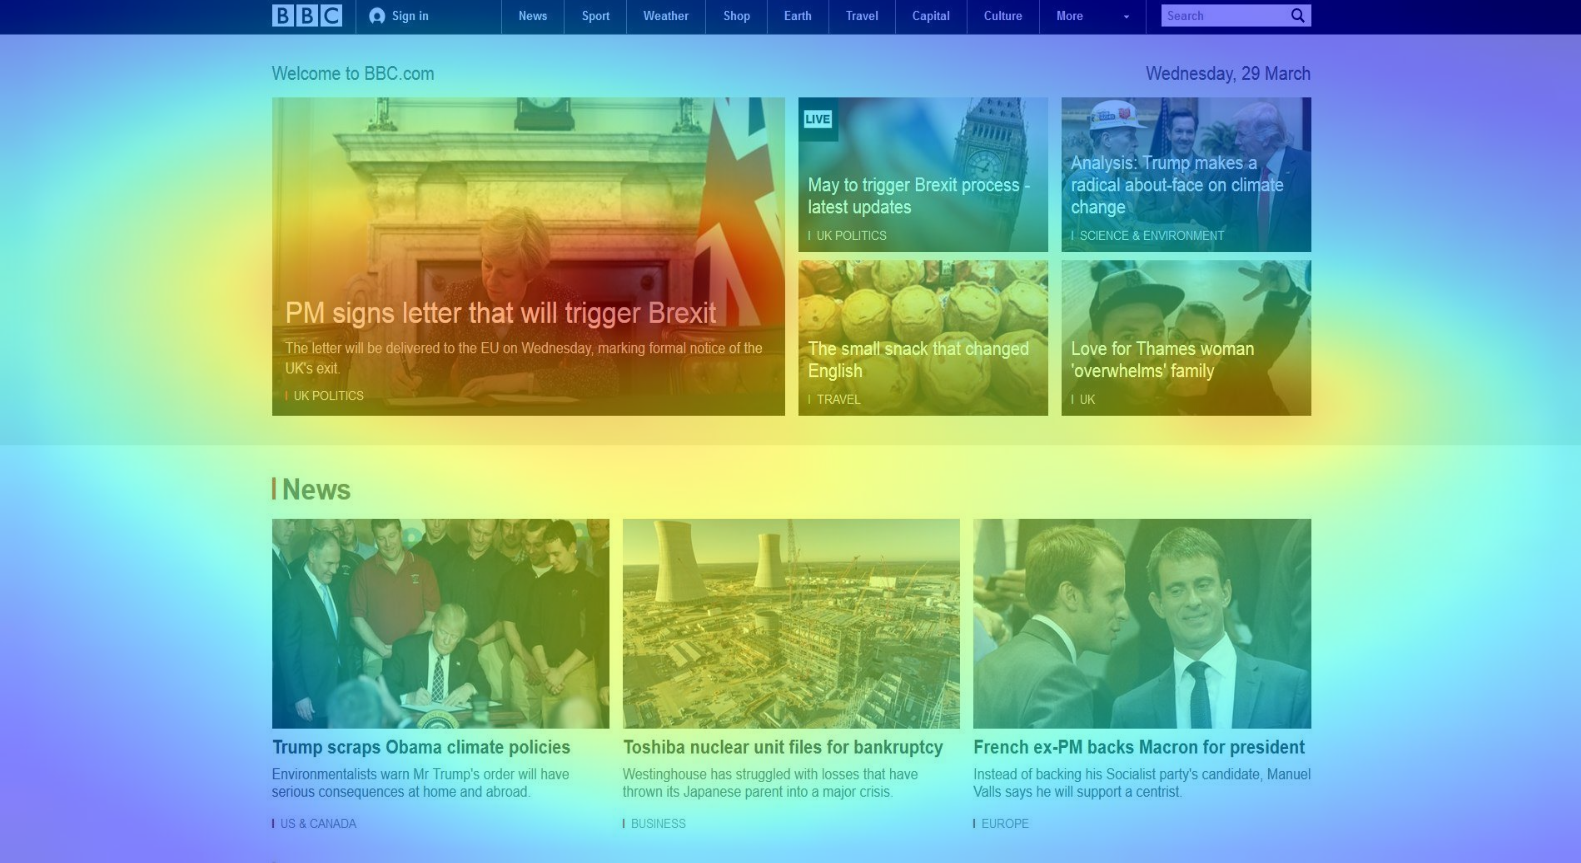
\includegraphics[scale=1, width = 4cm, height = 2.5cm]{final_test_3.png}
			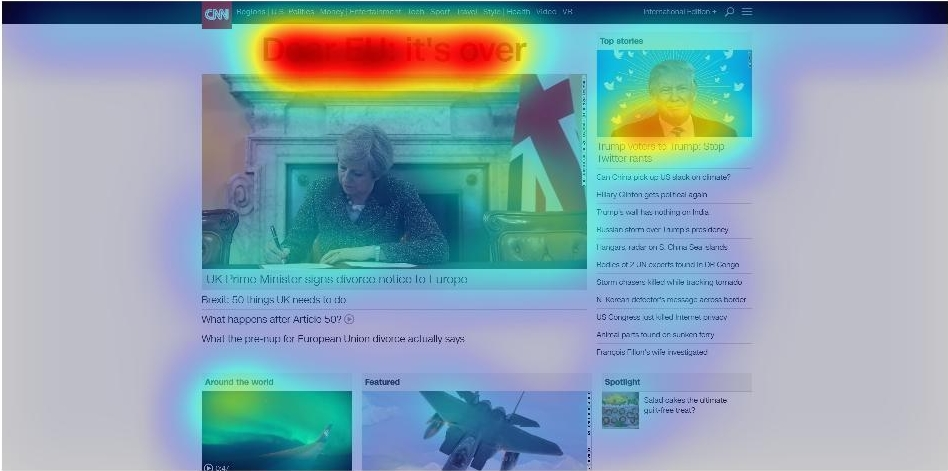
\includegraphics[scale=1, width = 4cm, height = 2.5cm]{itti_cnn.jpg}
			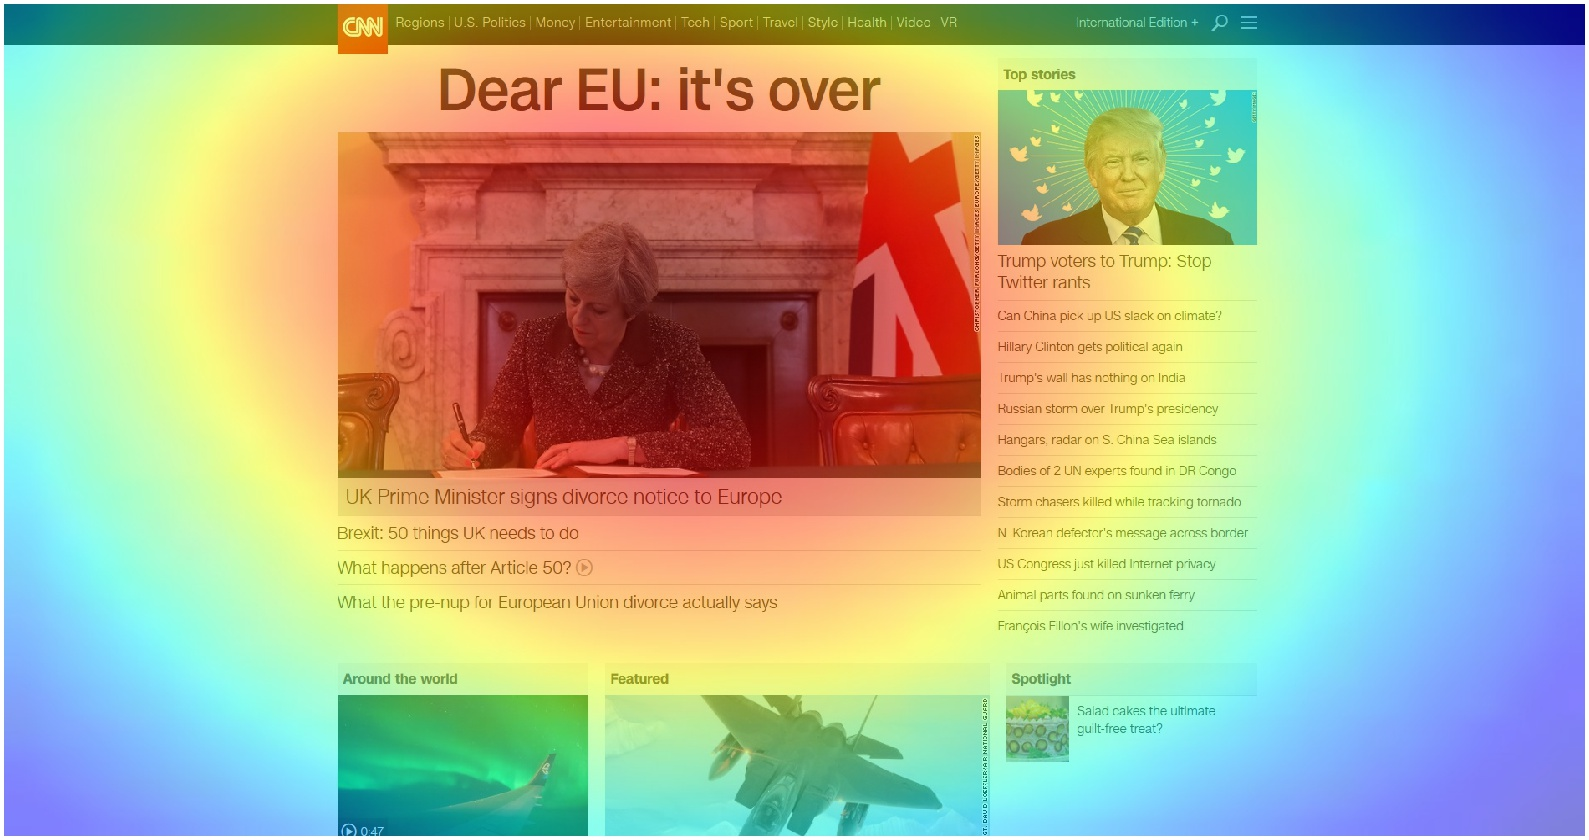
\includegraphics[scale=1, width = 4cm, height = 2.5cm]{prediction_for_cnn.jpg}			
		\end{center}
		\begin{center}
			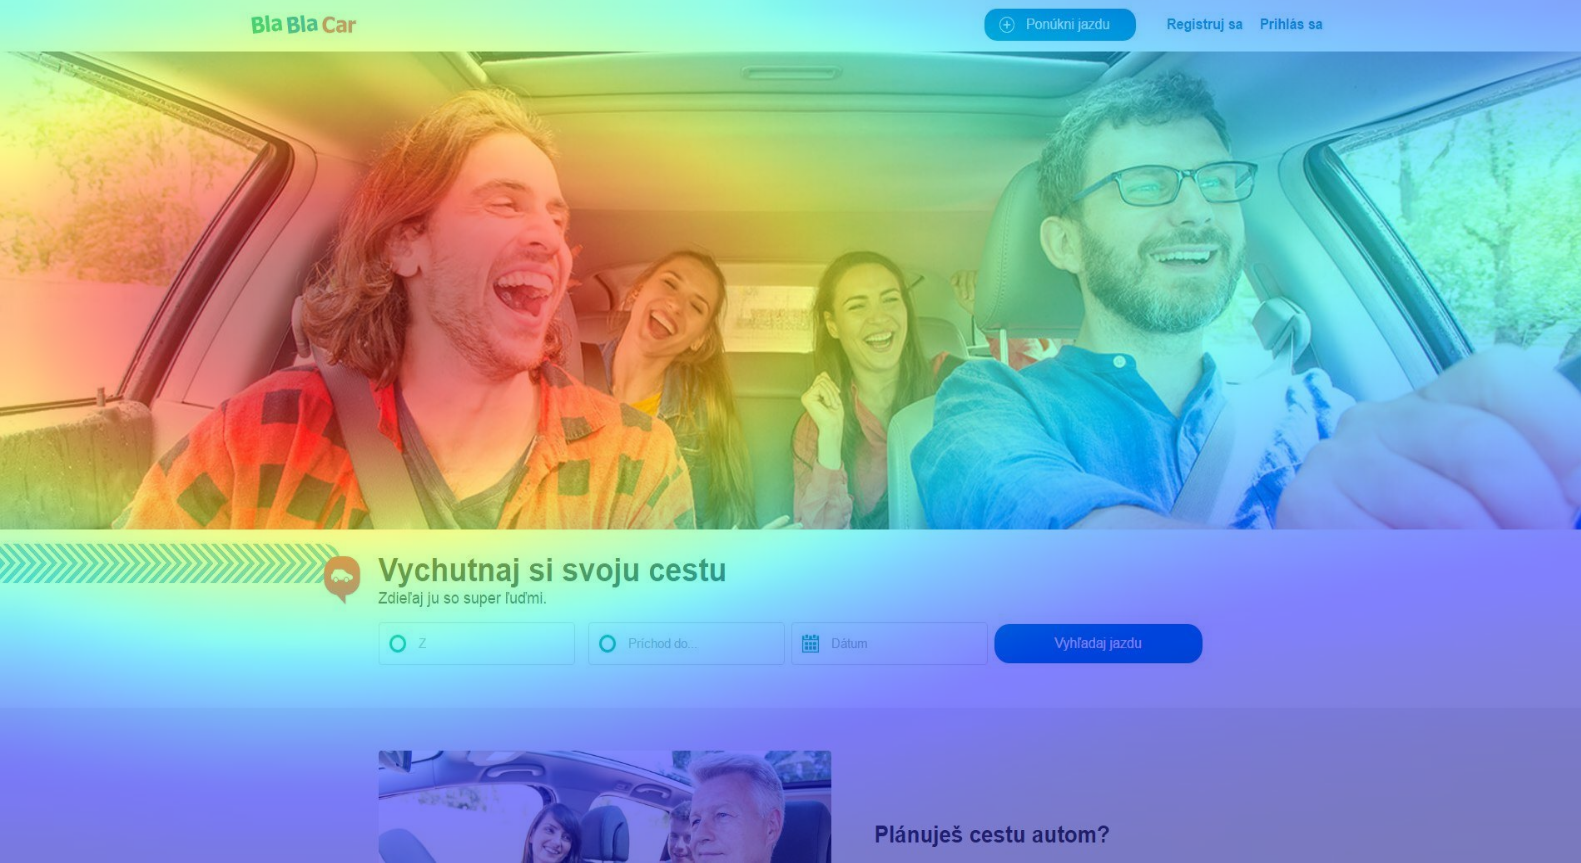
\includegraphics[scale=1, width = 4cm, height = 2.5cm]{hm_31.png}
			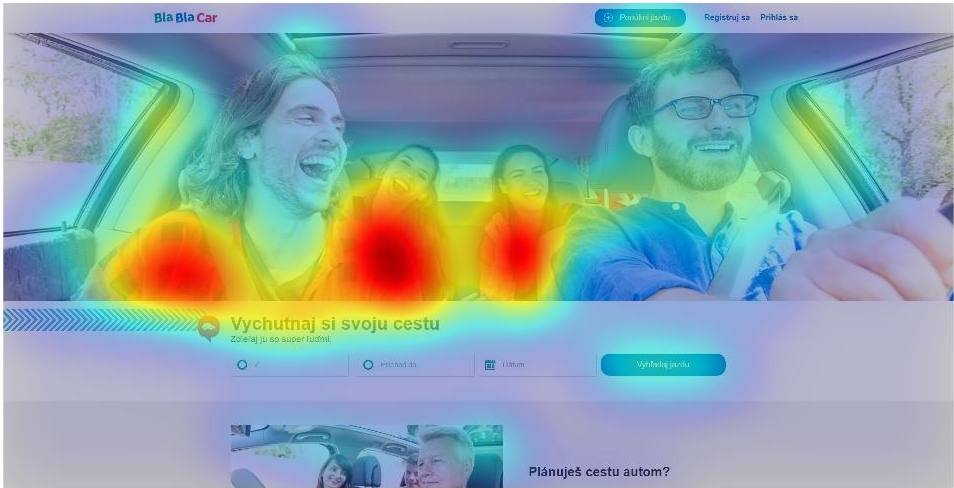
\includegraphics[scale=1, width = 4cm, height = 2.5cm]{itti_blablacar.jpg}
			\includegraphics[scale=1, width = 4cm, height = 2.5cm]{prediction_for_blablacar.JPG}			
		\end{center}
		\begin{center}
			\includegraphics[scale=1, width = 4cm, height = 2.5cm]{original_5.png}
			\includegraphics[scale=1, width = 4cm, height = 2.5cm]{itti_5.jpg}
			\includegraphics[scale=1, width = 4cm, height = 2.5cm]{prediction_for_vk.jpg}			
		\end{center}
		\caption[Náš model vs. Itti-ho model]{
			Grafická vizualizácia porovnania predikciíí Itt-ho modelu s naším. Vľavo mapy výraznosti vypočítané z reálnych fixácií ľudí, v strede predikcia pomocou Itti-ho modelu, vpravo predikcia nášho modelu.
		}\label{fig:itti_vs_my}
	\end{figure}

Na obrázku je možné pozorovať, že v niektorých situáciách je náš model presnejší, v iných nie. Naša neurónová sieť sa naučila predikovať primárne do strednej hornej oblasti, čo však na väčšine typov stránok je aj reálne prvá oblasť, ktorú vnímame. 

Najideálnejšie by bolo náš model porovnať s modelom od Chengyao Shen a Qi Zhao\cite{singapur_model}, popísaným v časti \ref{singapur}, ale ich dataset ani riešenie nie sú verejne dostupné. Hodnoty metrík preto nie sú vypočítané na tých istých dátach a porovnanie môže byť trochu zavádzajúce, prakticky ale náš model dosiahol hodnoty CC zhruba o 0.06 vyššie, sAUC je na tej istej úrovni a NSS má náš model o polovicu nižší, je to jediná metrika kde sme výrazne horší ako ich model. 

%%
%% Conclusion
%%
% TODO zvazit ci nedat do pice

\newpage
\section{Zhrnutie}

Vypracovaný diplomový projekt k problematike predikcie vizuálnej pozornosti sa venuje najmä jej časti berúcej do úvahy sémantický kontext scény s názvom pozornosť zhora nadol (z angl. top-down). Po preštudovaní uvedenej oblasti, dostupných datasetov  a existujúcich riešení, s dôrazom na najnovšie prístupy využívajúce strojové učenie a neurónové siete, sme navrhli sériu modelov, s ktorými sme neskôr experimentovali.

V prvotných experimentoch sme sa snažili využiť rôzne kombinácie datasetov, nakoniec nám ale ako najlepšie vyšlo použiť iba jeden, z dôvodu prílišnej rôznorodosti dát v nich (rôzne veľkosti obrázkov, zozbierané počas rôznych experimentov, atď.). Naša voľba pôvodne padla na DUT-OMRON, neskôr sme ale skončili pri datasete SALICON - ten je rozsiahlejší a o niečo lepšie spracovaný. Na ňom sme trénovali navrhnuté modely, najlepšie z nich vyšiel koncept kombinácie autoenkóderu s konvolučnými vrstvami VGG16 siete pre detekciu objektov, kedy práve časť VGG16 siete fungovala ako samostaný model, ktorého predikcie sa v rámci dekóderu spájali s tými z enkóderu. Týmto spôsobom sa nám podarilo dostať do siete informáciu o pozícii objektov, čo sa prejavilo aj na zlepšení samotných predikcií máp vizuálnej pozornosti. Tie sme nakoniec porovnávali s predikciami dvoch existujúcich modelov vizuálnej pozornosti.

Porovnávanie prebiehalo s modelom pre redukciu sémantických medzier (popísaný v kapitole \ref{semantic_gap}) s modelom SAM (popísaný v kapitole \ref{sam}). Porovnávané boli hodnoty metrík na troch datasetoch, SALICON, MIT1003 a CAT2000. Ako základný model pre naše riešenie sme zvolili ten natrénovaný práve na datasete SALICON, pri čom sme potom postupne dotrénovali sieť na zvyšné dva. Dosiahnuté hodnoty sa vo väčšine prípadov blížili hodnotám spomínaných riešení, ale len zriedkavo boli vyššie. To dokazuje, že zvolený prístup bol správny a predikcie sú konkurencie schopné, stále nie sú však najlepšie možné a je čo vylepšovať. Určite by sa dalo ďalej experimentovať práve s časťou pre detekciu objektov, v prípade možnosti trénovania na väčších grafických kartách by napríklad bolo možné zapojiť VGG16 časť do dekóderu skôr a tým získať väčšie množstvo trénovateľných parametrov, ktoré by potencionálne mohli zachytiť viac závislostí sémantického kontextu. Rovnako by dosť mohol pomôcť vačší dataset, ideálne čo najrozmanitejší (aj vnútorné aj vonkajšie exteriéry, príroda, mesto, ľudia, atď.) - tu by sa dalo uvažovať o vlastných experimentoch, tie sú ale dosť časovo náročné a vyžadujú značný počet participantov.


%%
%% References
%%
 \cleardoublepage
 \newpage
\newpage
\addcontentsline{toc}{section}{\refname}
\bibliographystyle{plain}
\bibliography{references}

%%
%% Appendix
%%
\ifthenelse {\boolean{bachelor}}
{
	
}
{
	\ifthenelse {\boolean{english}}
	{
		\renewcommand{\appendixname}{Appendix}
		\renewcommand{\appendixtocname}{Appendix}
	}
	{
		\renewcommand{\appendixname}{Príloha}
		\renewcommand{\appendixtocname}{Prílohy}
	}
	\pagenumbering{bychapter}
}
 \cleardoublepage
 \newpage
\appendix
\newpage
\null
\thispagestyle{empty}
\newpage
\pagestyle{plain}
\pagenumbering{roman}
%\renewcommand{\thepage}{\Alph{page}}

%TODO dat do pice
\section{Plán ďalšej práce}

Plán a rozdelenie práce na skúškové obdobie a ďalší semester:

\begin{itemize}
	\item refaktorizácia a upratanie doterajšej práce (kód, dokumentácia)
	\item experimentácia s neurónovou sieťou - autoenkóderom
	\item postupné dodávanie ďalších informácií o scéne sieti - pre začiatok poloha objektov
	\item pripravenie experimentu pre získanie dát pre pozornosť zhora nadol (top-down)
	\item vykonanie experimentu s čo najväčším počtom ľudí
	\item vyhodnotenie
	\item otestovanie ďalších faktorov pozornosti zhora nadol
	\item experimentovanie
	\item refactor kódu
	\item porovnanie výsledkov s inými riešeniami
	\item predbežné doplnenie dokumentácie
\end{itemize}

V závislosti od problémov a dosiahnutých výsledkov počas semestra sa bude plán predbežne meniť a upravovať.

\newpage
\pagestyle{plain}
\pagenumbering{roman}
%\renewcommand{\thepage}{\Alph{page}}

%TODO upravit - pridat dataset, ulozene modely, atd. 
\section{Obsah priloženého elektronického nosiča}

Štruktúra dát na elektronickom nosiči:

\begin{itemize}
	\item \textbf{dataset} - vzorka upraveného pripraveného datasetu pre neurónovú sieť
	\item \textbf{source\_codes} - zdrojové kódy
	\item \textbf{document} - pdf verzia odovzdávanej práce
\end{itemize}

%TODO zvazit pridanie casi s velkym diagramom architektury

%TODO Technicka dokumentacia? prostredie, hardver, kniznice, atd.

%TODO pouzivatelska prirucka

%TODO plan prace na riesenie projektu? 


\end{document}

%%%%%%%%%%%%%%%%%%%%%%%%%%%%%%%%%%%%%%%%%%%%%%%%%%%%%%%%%%%%%%%%%%%%%%%%%%%%%%%%%%%%%%%%

%%
%% !!!! set your own details
%%
\begin{comment}
[x] [Autor Dokumentu], [Nazov Stranky], [URL], [Datum Navstevy]
\end{comment}